%*************************************************************************
%	PLANTILLA PARA LA EDICIÓN DE PROYECTOS FIN DE CARRERA
%	Departamento de Teoría de la Señal y Comunicaciones
%	Universidad de Alcalá
%*************************************************************************

%******************
%Tipo de documento
%******************
\documentclass[12pt]{book}

%********************
%Paquetes a utilizar
%********************
\usepackage[square,numbers]{natbib}
\usepackage[T1]{fontenc}
\usepackage[spanish]{babel}
\usepackage{verbatim}
\usepackage{amssymb}
\usepackage{amsmath}
\usepackage{fancyhdr}
\usepackage{graphicx}
\usepackage{multicol}
\usepackage{makeidx}
\usepackage[bf,SL,BF]{subfigure}
\usepackage[utf8]{inputenc}
\usepackage{longtable}
\usepackage{anysize}

%*************
%Definiciones
%*************
\deactivatetilden 
\addto\captionsspanish{\def\tablename{Tabla}\def\listtablename{Lista
de tablas}\def\listfigurename{Lista de figuras}}
%Cambios en los márgenes
%\renewcommand{\baselinestretch}{1.1}

\setlength{\oddsidemargin}{0.4cm}
\setlength{\evensidemargin}{0.4cm} 
\setlength{\headsep}{0.4cm}
\setlength{\textheight}{23cm} \setlength{\textwidth}{16cm}
\setlength{\topmargin}{-0.25cm}\flushbottom



%***************
%Título del TFC
%***************
\title{SNSAngelGuard}

%****************
%Autor
%****************
\author{José Javier Blecua de Pedro}

%Prepara el índice
\makeindex

%***********************
%Comienzo del documento
%***********************
\begin{document}
\setcounter{tocdepth}{4} \setcounter{secnumdepth}{3}

\frontmatter

%Incluimos fichero previo.tex -> genera la hoja de calificación
\begin{titlepage}
%**********************************************************
%GENERA LA HOJA OFICIAL DE CALIFICACIÓN PARA PROYECTOS FIN DE CARRERA
%SEGÚN EL FORMATO DE LA UNIVERSIDAD DE ALCALÁ Y DEL DEPAR-
%TAMENTO DE TEORÍA DE LA SEÑAL Y COMUNICACIONES.
%**********************************************************

\begin{center}
\Large \textsc{Universidad de Alcalá}\\
\vspace{0.5cm}

%Nombre de la escuela-> seleccione el que corresponda.
\textbf{Escuela Técnica Superior de Ingeniería Informática}\\
%\textbf{Escuela Técnica Superior de Ingeniería Informática}\\

%Titulación -> escriba su titulación
Ingeniero Técnico en Informática de Sistemas\\
\end{center}

\vspace{0.5cm}

\begin{center}
%Para compilar con latex

\includegraphics[width=4cm]{Figuras/LogoUAH.eps}\\
%Para compilar con pdflatex
%
\includegraphics[width=4cm]{Figuras/LogoUAH.png}\\
\end{center}


\begin{center}
\vspace{1cm}

\Large Proyecto Fin de Carrera\\
\textbf{\Large {{SNSAngelGuard}}}\\
\vspace{1cm}
\large Autor: José Javier Blecua de Pedro\\
Director: Miguel Angel Sicilia Urbán\\
\vspace{0.5cm}
\end{center}

\begin{flushleft}
\textbf{TRIBUNAL:}\\
\vspace{1.5cm}
\textit{Presidente: D. Nombre y apellidos del presidente}\\
\vspace{1.5cm}
\textit{Vocal 1º: D. Nombre y apellidos del vocal 1}\\
\vspace{1.5cm}
\textit{Vocal 2º: D. Nombre y apellidos del vocal 2}\\
\vspace{1.5cm}
\textbf{CALIFICACIÓN:}............................................................ FECHA:.................... \\
\end{flushleft}

%Final de la hoja de calificación.

\end{titlepage}

%Prepara el título del proyecto.
\maketitle

%Incluye las dedicatorias (fichero dedicatorias.tex)
\begin{flushleft}
\textit{Aquí escribes las dedicatorias.}
\end{flushleft}

%Incluye los agradecimientos (fichero agradecimientos.tex)
\chapter{Agradecimientos}
Siempre hay alguien a quien agradecerle algo, y más cuando has hecho un Proyecto Fin de Carrera (PFC).

%Incluye el resumen del Proyecto fin de carrera (fichero resumen.tex)
\chapter{Resumen}
SNSAngelGuard es un software desarrollado por la Universidad de Alcalá cuyo objetivo es controlar la actividad de una determinada persona o perfil dentro de la Red Social Facebook.  Una figura denominada Tutor controlará, por medio de informes generados desde SNSAngelGuard, la actividad que un usuario pueda generar en dicha red social. Los filtros actuales dentro de la aplicación permiten controlar los mensajes que se escriben dentro del muro, la edad de amigos potencialmente peligrosos, su configuración de seguridad y el número de visitas que recibe una determinada persona o perfil de Facebook. Con ésta implementación se consigue controlar determinados acosos por terceras personas que el usuario pueda recibir y a su vez, notificarse automáticamente a su Tutor. Esta aplicación se ejecutará en el entorno de Facebook y utilizará una base de datos externa que, mediante servicios RestFul, controlará el tráfico de datos del usuario y servirá como base de análisis a la aplicación.

\chapter{Abstract}
SNSAngelGuard is a softwer developed for the University of Alcala de Henares and its objetive is controling the activity of a determinate Facebook usser or his/her profile within this social network. A feature called Tutor, will control, through generated researchs from SNSAngelGuard, the activity that a usser could develop in this social network. The current filters within the aplication allow the control of the messages posted on the wall, the age of the potential dangerous friends, the security settings and the number of visits this usser or Facebook profile can recive. With this implementation the application takes control of possible harrasments by third people and at the same time, it communicates them automatically to the Tutor. This application will be run in the Facebook enviroment and it will  use an external database which, by using RestFul services, will protect the usser data traffic and will work as a base for the application analysis.


%Incluimos lista de abreviaturas y de símbolos si es necesario.
%\include{abreviaturas}
%\include{simbols}

\mainmatter

%Inlcuimos el índice que latex genera automáticamente.
\tableofcontents
%La lista de figuras incluidas en el proyecto.
\listoffigures
%La lista de tablas.
\listoftables



%Incluimos los capítulos del proyecto. Cada capitulo se encuentra en un fichero tex,
%que insertamos en el documento por medio del comando \include{capitulo-cualquiera}

%Incluye Introducción (fichero introduccion.tex)
% Formato para un capítulo cualquiera

%Título del capítulo
\chapter{Introducción.} 

\section{Qué es SNSAngelGuard}
SNSAngelGuard es una herramienta software diseñada en la Universidad de Alcalá en colaboración con otras universidades a nivel nacional con el objetivo de crear una aplicación que permita profundizar en el amplio universo de las redes sociales. Este proyecto forma parte de un proyecto global cuyo objetivo es desarrollar herramientas para simular el comportamiento de una Red Social, sea cual fuere su naturaleza, y comprender su comportamiento, por medio de modelado de datos y construcción de protocolos.En este proyecto se pretenden dos objetivos:

\begin{enumerate}
\item Construcción de un modelo de datos general para el conjunto de redes sociales existentes, haciendo un estudio de aquellas partes en las que dichas redes sociales pueden llegar a un punto en común en el almacenamiento de datos.
\item Diseñar y desarrollar una aplicación que extraiga datos de una determinada Red Social y que trate dichos datos con una funcionalidad determinada. En éste caso, la red social a tratar será Facebook.
\end{enumerate}


\section{Concepto de Red Social}
Como concepto, una Red Social puede entenderse como un ente formado por un conjunto de personas que comparten algún tipo de relación (familiares, amigos, trabajo, ocio..., etc.) o simplemente, por personas que quieren compartir su conocimiento para llevar a cabo un objetivo común. Dentro de una Red Social, cada persona puede comunicarse con las personas que forman su entorno, además de tener nuevas relaciones y darse a conocer dentro de otros entornos que a su vez, todos juntos, conformen dicha red.
\bigskip
\par
Las redes sociales tienen su origen en la teoría de los “Seis grados de separación”. Esta teoría se basa en la idea de que una persona puede estar conectada con cualquier otra persona del planeta a través de una cadena de no más de seis intermediarios. Dicho de otra forma, las redes sociales se basan en el simple hecho de que el número de conocidos crece exponencialmente con el número de enlaces de la cadena, y sólo un pequeño número de enlaces son necesarios para que el conjunto de conocidos se convierta en una población humana entera.
\bigskip
\par
Si ponemos ésta idea en práctica, podemos comprobar que no es nada descabellada. Cada persona se suele relacionar con aproximadamente unas 100 personas, entre familiares, amigos, compañeros de trabajo,..., etc. Si cada una de estas personas se relaciona con otras 100 personas no comunes, no es difícil imaginarse que una persona puede difundir un mensaje entre 10000 personas. Si seguimos recorriendo eslabones en la cadena de relaciones, en unos cuantos pasos estaríamos preparados para mandar un mensaje a cualquier persona que estuviera conectada a una Red Social. Dicho de otra manera, estaríamos preparados para
entrar en contacto con cualquier persona del planeta.
\bigskip
\par
El verdadero impacto que tiene una Red Social sobre la sociedad actual moderna no tiene límites. Nos encontramos ante un fenómeno de masas, con una capacidad de comunicación imposible de calcular. Por esta razón, el estudio de las Redes Sociales se ha
convertido en un elemento esencial para las Universidades y Centros de Conocimiento y, sin ir más lejos, para todas aquellas empresas, tanto grandes, medianas o pequeñas, que quieran expandirse y dar a conocer sus productos. Cualquier departamento de marketing incorpora especialistas en redes sociales para calcular el impacto de sus productos en la sociedad y difundirlos de la manera más eficaz posible.
\bigskip
\par
Evidentemente, todas estas relaciones serían imposibles sin un vehículo idóneo de comunicación. Gracias al desarrollo tecnológico del sector de la informática y de las telecomunicaciones, cualquier persona puede disponer de un equipo informático
moderadamente asequible y una conexión a Internet lo suficientemente rápida como para poder estar en constante comunicación con otra, y poder enviar y recibir mensajes simultáneamente, como si ésta comunicación se produjera “cara a cara”.
\section{OpenSocial}
OpenSocial es un conjunto de API comunes destinadas a la creación de aplicaciones sociales en múltiples sitios web. OpenSocial está compuesto por API de JavaScript y API de datos de Google. La existencia de este modelo de programación único resulta de gran utilidad tanto para los desarrolladores como para los sitios web. 
\bigskip
\par
En primer lugar, los desarrolladores sólo tienen que aprender las API una vez para crear aplicaciones que funcionen con cualquier sitio web compatible con OpenSocial. 
\bigskip
\par
En segundo lugar, como cualquier sitio web puede implementar OpenSocial, los desarrolladores disponen de una amplia red de distribución para llegar a los usuarios. Los sitios web también se benefician mediante la participación de un conjunto mucho más numeroso de desarrolladores externos que el que podrían conseguir sin un conjunto estándar de API. 
\bigskip
\par
La Compañía Google y sus asociados, ofrecen algunas tecnologías para que Internet en su conjunto llegue a ser un medio más social, respondiendo así al claro interés de los usuarios. Productos, como orkut, son sólo uno de los distintos sitios web que implementan OpenSocial. Actualmente, el código de ejemplo se ofrece con la licencia de Apache 2.0. Además, las licencias de toda la documentación de OpenSocial proceden de Creative Commons, por lo que se puede reutilizar y combinar los servicios como estimes oportuno. En el futuro, se plantea ofrecer el software libre de los componentes necesarios para ejecutar OpenSocial en tu propio sitio web.
\subsection{Estructura básica de una aplicación que utiliza el API de OpenSocial}
Las aplicaciones de OpenSocial utilizan la estructura de gadgets de Google, pero con extensiones que proporcionan acceso programático a datos sociales dentro de su entorno de contenedor. De forma similar a los gadgets de Google, las aplicaciones de OpenSocial alojan documentos XML con lenguaje HTML/JavaScript integrado. Las aplicaciones sociales disponen de la mayor parte de la infraestructura de los gadgets de Google, pero con algunas pequeñas excepciones. Uno de los primeros entornos de las aplicaciones sociales que utilizan las API de OpenSocial es orkut. Se espera que otros sitios web compatibles con OpenSocial admitan pronto la participación de desarrolladores.
\subsection{Crear aplicaciones con OpenSocial}
Las aplicaciones sociales se crean en principio de la misma forma que los gadgets de Google: con tu editor de texto favorito o con el Editor de gadgets de Google. A continuación, se pueden aumentar con las API JavaScript de OpenSocial, donde estas aplicaciones pueden obtener y enviar datos sociales sobre amigos y actividades.

\section{Facebook}
Facebook es el ejemplo de Red Social, mundialmente conocido. Facebook es una aplicación que engloba una conjunto de redes sociales creada por
Mark Zuckerberg. Se trata de una aplicación web en la cualquier usuario puede acceder a ella a través de únicamente una dirección de correo válida. En ella, el usuario puede ponerse en contacto con otros usuarios de una o más redes sociales, dependiendo de su situación académica, su lugar de trabajo o su región geográfica.
\bigskip
\par
Originalmente se creó específicamente para estudiantes de Harvard, Universidad en la que inició sus estudios su creador, pero posteriormente, tras su éxito a nivel mundial, fue ampliada a cualquier persona que tuviera una dirección de correo electrónico.
\bigskip
\par
Una de las características principales de Facebook es su expansión hacia el mundo de las aplicaciones web. Se ha convertido en una plataforma en la que terceros pueden desarrollar aplicaciones y hacer negocio a partir de la red social.
\bigskip
\par
Para conseguir dicho objetivo, el equipo de Facebook ha ido publicando diferentes APIs, basadas en Servicios Web, para la creación de aplicaciones y el acceso a datos de usuario, las cuales van adaptándose a las tecnologías actuales y marcando un perfil de aplicación determinado. Cualquier desarrollador tiene acceso a ellas y constituyen una de las mayores riquezas actuales de la compañía.
\bigskip
\par
Actualmente, un desarrollador puede empezar una aplicación enfocándola directamente sobre el tipo de dispositivo para el que va dirigido. Las interfaces
publicadas por Facebook así lo establecen, dejando a la elección del programador el tipo de aplicación que desea realizar, tales como páginas web, aplicaciones para dispositivos móviles o aplicaciones para escritorio.
\subsection{Tipos de APIs}
Actualmente, Facebook dispone de las siguientes interfaces para el desarrollo de
aplicaciones:
\begin{enumerate}
\item Login: Es una interfaz que integra los métodos de logueo necesarios para una aplicación web. Puede ser utilizada desde cualquier lenguaje de programación pero es excesivamente sencillo de utilizar en el lenguaje JavaScript.
\item GraphApi: Es la interfaz más utilizada y más universal. Permite acceder a los datos de un usuario por medio de objetos o entidades que pueden ser tratadas posteriormente a través de la aplicación.
\item FQL: Son las siglas de Facebook Query Language o, dicho de otra manera, es el lenguaje de SQL de Facebook para el acceso a datos de usuario.
\item Legacy REST API: Es el conjunto de servicios REST que Facebook puso en
disposición para el acceso a datos mediante peticiones HTTP. Es el más antiguo de
todos y está próximo a la desaparición.
\end{enumerate} 

\subsection{RestFB}
En la actualidad, el creciente volumen de desarrolladores que trabajan en proyectos de aplicaciones de Facebook ha desencadenado una oleada de apariciones de arquitecturas o proyectos que encapsulan el acceso a las interfaces ofrecidas por Facebook y hacen más fácil trabajar con esta. Con estas nuevas arquitecturas, se ofrece el acceso a toda la funcionalidad de Facebook mediante clases de cualquier lenguaje de programación. RestFB es una de estas arquitecturas.
\bigskip
\par
RestFB engloba las APIs de Facebook Grap API y Old REST API mediante un cliente escrito en el lenguaje de programación JAVA. Tiene las siguientes características:
\begin{enumerate}
\item Es totalmente transparente a la interfaz que se utiliza para el acceso a datos de Facebook. El programador no conoce con certeza qué interfaz se está utilizando.
\item Su api es mínima, ya que engloba una serie de métodos públicos que son configurables utilizando las sentencias FQL proporcionadas por Facebook, por lo que los métodos definidos en sus interfaces son realmente pocos.
\item Los cambios que se pueden producir por parte de Facebook en su interfaz son automáticamente absorbidos, haciendo que el usuario no cambie su forma de
desarrollar la aplicación.
\item Para configurarlo, no hay más que introducir su dependencia Maven correspondiente en el pom.xml del proyecto.
\item No guarda dependencias con ningún otro módulo.
\item El transporte de datos se realiza mediante lenguaje XML o JSON, pudiendo ser parseado al llegar a la aplicación dependiendo de las necesidades funcionales del módulo.
\end{enumerate} 
Por todas estas razones, esta arquitectura ha sido la elegida para llevar a cabo las interacciones con Facebook desde SNSAngelGuard.

\section{Servicios Web}
\subsection{¿Qué es un Servicio Web?}
El consorcio W3C\footnote[1]{World Wide Web Consortium: Comunidad internacional que desarrolla estándares que aseguran el crecimiento de la Web a largo plazo. Fuente www.w3c.es} define a los Servicios Web como sistemas software diseñados para soportar una interacción interoperable maquina a máquina sobre la red. Dichos servicios suelen ser presentados en forma de APIs Web que pueden ser accedidas en una red (principalmente Internet) por medio de una aplicación y se suelen ejecutar en la máquina que los aloja.
\bigskip
\par
Hay muchas definiciones para éstos servicios pero la idea general se refiere a clientes  y servidores que se comunican entre sí mediante mensajes XML\footnote[2]{Son las siglas de Extensible Markup Language, una especificación/lenguaje de programación desarrollada por W3C. XML es una versión de SGML, diseñado especialmente para documentos de la red. Permite que los desarrolladores creen sus propias etiquetas, permitiendo la definición, transmisión, validación e interpretación de datos entre aplicaciones y entre organizaciones.} los cuales siguen el estándar SOAP\footnote[3]{Son las siglas de Simple Object Access Protocol. Protocolo estándar que define cómo dos objetos en diferentes procesos pueden comunicarse por medio de intercambio de datos XML.}.
\bigskip
\par
En estos últimos años, se ha popularizado una arquitectura de Servicio Web denominada REST\footnote[4]{Son las siglas de Representational State Transfer.}. Esta arquitectura se ha convertido en una nueva opción para decantarse por tecnología basada en Servicios Web. En éste caso, tenemos tres opciones:
\begin{enumerate}
\item Llamadas a Procedimientos Remotos (RPC, Remote Procedure Call): Estos servicios presentan una interfaz de llamada a procedimientos y funciones distribuidas, lo cual es muy familiar a la mayoría de los desarrolladores. Normalmente, la unidad básica de uso de éste servicio es la operación WSDL\footnote[5]{Son las siglas de Web Service Description Language, un formato XML que se utiliza para describir Servicios Web. Describe la interfaz pública de un Servicio Web. Está basado en XML y describe la forma de comunicación, es decir, los requisitos del protocolo y los formatos de mensaje necesarios para interactuar con los servicios listados en su catálogo. Las operaciones y mensajes que soporta se describen en abstracto y se ligan después al protocolo concreto de red y al formato del mensaje.}.
\bigskip
\par
Las primeras herramientas para Servicios Web estaban centradas en éste tipo de enfoque, es por esta razón que son denominados Servicios Web de primera generación y su uso está muy extendido. Sin embargo, ha sido ampliamente criticado y muchos expertos creen que debería desaparecer, ya que su implementación se basa en el mapeo de servicios directamente a funciones específicas del lenguaje o llamadas a métodos.
\item Arquitectura Orientada a Servicios SOA\footnote[6]{Son las siglas de Service Oriented Architecture.}: Según la arquitectura de llamadas a Procedimientos Remotos, la unidad básica de operación es la Operación. En el caso de los Servicios SOA, se trata de implementar Servicios Web a través del mensaje, que en éste caso será la unidad básica de operación. Esta arquitectura también es conocida como Servicio Orientado a Mensajes.
\item Servicios REST: Son Servicios Web que intentan basarse en protocolos HTTP o similares. Su objetivo es restringir el uso de una interfaz a un conjunto de operaciones estándar universalmente conocidas (GET, PUT, POST, DELETE). Por lo tanto, esta arquitectura se basa en interactuar con recursos con estado en vez de mensajes u operaciones. 
\end{enumerate}
\subsection{Arquitectura REST}
\subsubsection{Introducción}
REST es un estilo de arquitectura Software diseñado para el intercambio de datos en sistemas distribuidos. Fue introducido en la tesis doctoral de Roy Fielding en el año 2000, el cual es uno de los principales autores de la especificación HTTP.
\bigskip
\par
Los servicios REST se basan en el concepto  de “Todo recurso  (información) debe tener y ser accesible mediante una URI única”. A partir de éste concepto, se usan los métodos de comunicación web sobre HTTP (GET, PUT, POST, DELETE)  para definir diferentes acciones predefinidas sobre los recursos “URIs”.
Las características básicas de los servicios REST son los siguientes:
\begin{enumerate}
\item Todo recurso debe tener una URI única.
\item Los recursos son enlazados entre sí.
\item Uso de tecnología estándar (HTTP, XML, JSON,…, etc).
\item El recurso puede tener múltiples representaciones dependiendo de la solicitud.	
\end{enumerate}
La figura 1.1 representa la arquitectura de la tecnología REST:
\begin{figure}
\begin{center}
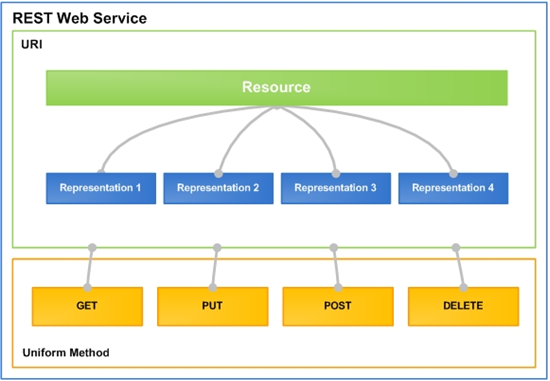
\includegraphics[width=12cm,height=8cm]{Figuras/REST.png}
\end{center}
\caption{\label{REST} Arquitectura de la tecnología REST}
\end{figure}
\subsubsection{Principios básicos}
\begin{enumerate}
\item Escalabilidad de la interacción con los componentes: Un determinado sitio web puede crecer exponencialmente sin degradar su rendimiento. Varios sistemas pueden acceder y utilizar servicios REST simultáneamente sin que esto degrade el rendimiento de la aplicación.
\item Interfaces estándar: Gracias al protocolo HTTP, cualquier cliente puede interactuar con un servicio REST sin necesidad de una configuración especial, únicamente definiendo la URI característica del propio recurso
\item Funcionamiento independiente de la arquitectura: Al ser una arquitectura basada en protocolos HTTP y estándares de intercambio de mensajes, permite adaptarse a cualquier tipo de cliente, ya que HTTP permite la extensibilidad mediante el uso de cabeceras a través de las URIs.
\item Es compatible con sistemas intermedios: Pueden ser utilizados en combinación con proxys para Web, herramientas de mejora de la seguridad, como firewalls y con herramientas de encapsulado para la Web, como es el caso de los gateways.  
\end{enumerate}
\bigskip
\par
REST logra conseguir estos objetivos aplicando las siguientes restricciones:
\begin{enumerate}
\item Identificación de recursos y manipulación de ellos a través de representaciones. Esto se consigue a partir de URIs. HTTP es un protocolo centrado en URIs. Los recursos son objetos lógicos que intercambian mensajes con las entidades que requieran sus servicios. No pueden ser directamente accedidos o modificados, más bien se trabaja con representaciones de ellos, es decir, cuando invocamos al método PUT para modificar los datos de un recurso, realmente estamos enviándole como mensaje una representación de lo que debería ser. Internamente, el recurso es totalmente transparente, es decir, puede desde un registro de una entidad de base de datos, un fichero plano…
\bigskip
\par
\item Mensajes autodescriptivos. REST establece que los mensajes HTTP deben ser tan descriptivos como sea posible. Esto hace que los intermediarios interpreten los mensajes y ejecuten los servicios en nombre del usuario. HTTP logra este objetivo por medio de una definición de un método estándar (GET, PUT, POST, DELETE), muchas cabeceras y un método de direccionamiento. Por ejemplo, las cachés Web saben que, por defecto, el método GET es cacheable, sin embargo, el método POST no lo es. Además, saben cómo interpretar la información contenida en las cabeceras, es por esta razón por la cual, cuando una aplicación accede a un recurso de una base de datos por medio de un servicio REST, el navegador es capaz de obtener el usuario el cual intenta acceder y modificar dicha base de datos por medio de su cabecera.
\bigskip
\par
\item Hipermedia como mecanismo de estado de la aplicación. El estado actual de una aplicación web es capturado mediante archivos de hipertexto que son alojados tanto en el cliente como en el servidor de la aplicación. El servidor conoce en todo momento el estado de los recursos pero no intenta seguir la pista a las sesiones individuales de cada cliente. Este trabajo es realizado por el navegador, quien sabe navegar de recurso en recurso, recogiendo la información que él necesita para cambiar de un estado a otro dependiendo del servicio REST que esté ejecutando en cada momento.
\end{enumerate}
\subsection{Funcionalidad}
La funcionalidad básica de un servicio web se encuentra en el diseño de una interfaz que defina los métodos de acceso a los recursos para el resto de aplicaciones desde el servidor de la aplicación. Tras el diseño, esta interfaz se hará pública y las aplicaciones  podrán hacer uso de todos sus recursos aplicando las restricciones que se han planteado anteriormente. 
Esta es precisamente, la arquitectura que se ha definido para SNSAngelGuard y que se procederá a describir en los capítulos posteriores.

%Incluye un capítulo cualquiera (capitulo-cualquiera.tex)
% Formato para un capítulo cualquiera

%Título del capítulo
\chapter{Arquitectura de SNSAngelGuard} 
%Sección primera
\section{Introducción}
SNSAngelGuard es una aplicación concebida como medio para realizar un ejemplo práctico sobre las investigaciones que pueden desarrollarse en una Red Social. En el presente documento, la red elegida es Facebook. Como se ha mencionado anteriormente, la base de datos de éstas investigaciones fue diseñada para albergar varias aplicaciones en las que estuvieran involucradas tambien redes sociales tales como Tuenti, Twitter, Open Social, ..., etc, por lo que la arquitectura de la base de datos no es exclusiva de SNSAngelGuard, pero sí que es totalmente compatible con Facebook.

\section{Diseño estructural}
La arquitectura se muestra en la figura 2.1. 
\bigskip
\par
\begin{figure}
\begin{center}
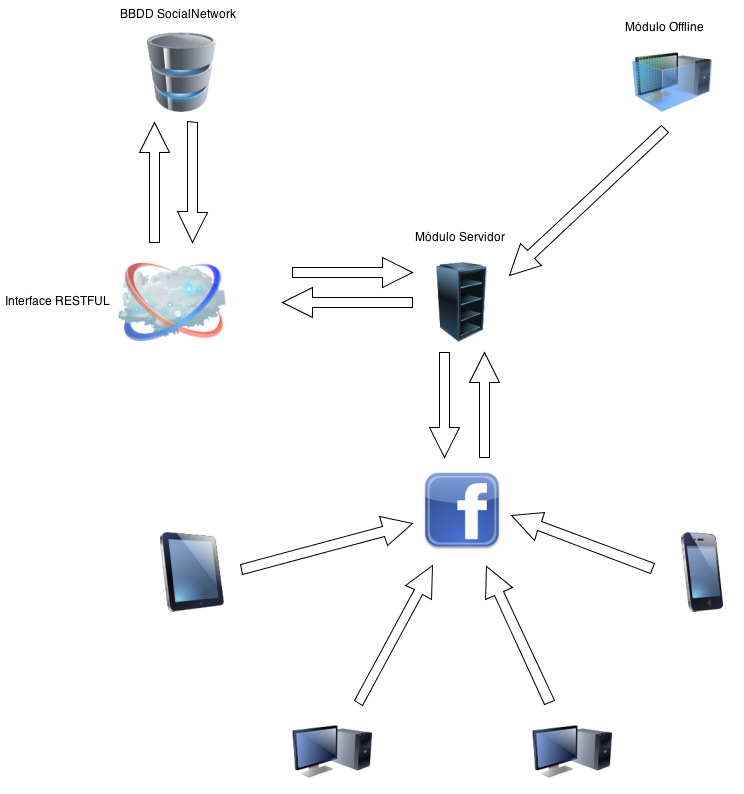
\includegraphics[width=12cm,height=10cm]{Figuras/ArchitectureSNS.png}
\end{center}
\caption{\label{Arquitectura} Arquitectura de la aplicación SNSAngelGuard}
\end{figure}
\bigskip
\par
Está conformada por una serie de módulos que se enumeran a continuación:
\begin{enumerate}
\item Base de Datos SocialNetwork: Contendrá todas las estructuras necesarias para acceder a cualquier funcionalidad de una Red Social. Guardará datos relacionados con su actividad, tales como datos a nivel personal, como pueden ser su fecha de nacimiento, su dirección, ..., etc., como datos a nivel de la propia Red Social, tales como sus amistades, sus relaciones personales con más miembros de dicha Red Social, sus comentarios en el muro, sus réplicas, enlaces a sus fotos o videos, ..., etc.
\item Interface RESTFUL: Este ente contendrá todas las estructuras necesarias para acceder a la base de datos por medio de Servicios Web. A través de éstas estructuras se creará una API que posteriormente se publicará para que todo aquel desarrollador que quiera utilizar esta base de datos pueda hacerlo como si se tratara de una API de una Red Social.
\item Módulo Servidor: Este módulo definirá una serie de estructuras que procesarán la información obtenida de los usuarios de la Red Social y, posteriormente, realizará las acciones propias de la aplicación, tales como el procesado de la información y la elaboración de informes para, posteriormente, ser enviados a los tutores del usuario en la aplicación.
\item Módulo Cliente: Está conformado por todos los dispositivos que pueden acceder a la Red Social y, a partir de ésta, ejecutar la aplicación SNSAngelGuard. Recordemos que ésta aplicación se ejecuta a través de Facebook, por lo que para acceder a ella, el usuario tendrá que tener un usuario válido dentro de ésta Red Social. Este módulo además, estará preparado para que cualquier dispositivo, sea cual fuere su naturaleza, pueda acceder a la aplicación y generar actividad a través de ella.
\item Módulo Offline: Este módulo, como su propio nombre indica, se ejecutará o podría ejecutarse, cuando un usuario no esté logueado dentro de Facebook. Estará conformado por una serie de procesos que realizan backups programados de la información del usuario en Facebook y elaborarán informes con la periodicidad indicada para cada tutor.
\end{enumerate}



\subsection{Estructura de la base de datos}
El modelo Entidad Relación que seguirá la base de datos es el que muestra la figura 2.2:
\bigskip
\par
\begin{figure}
\begin{center}
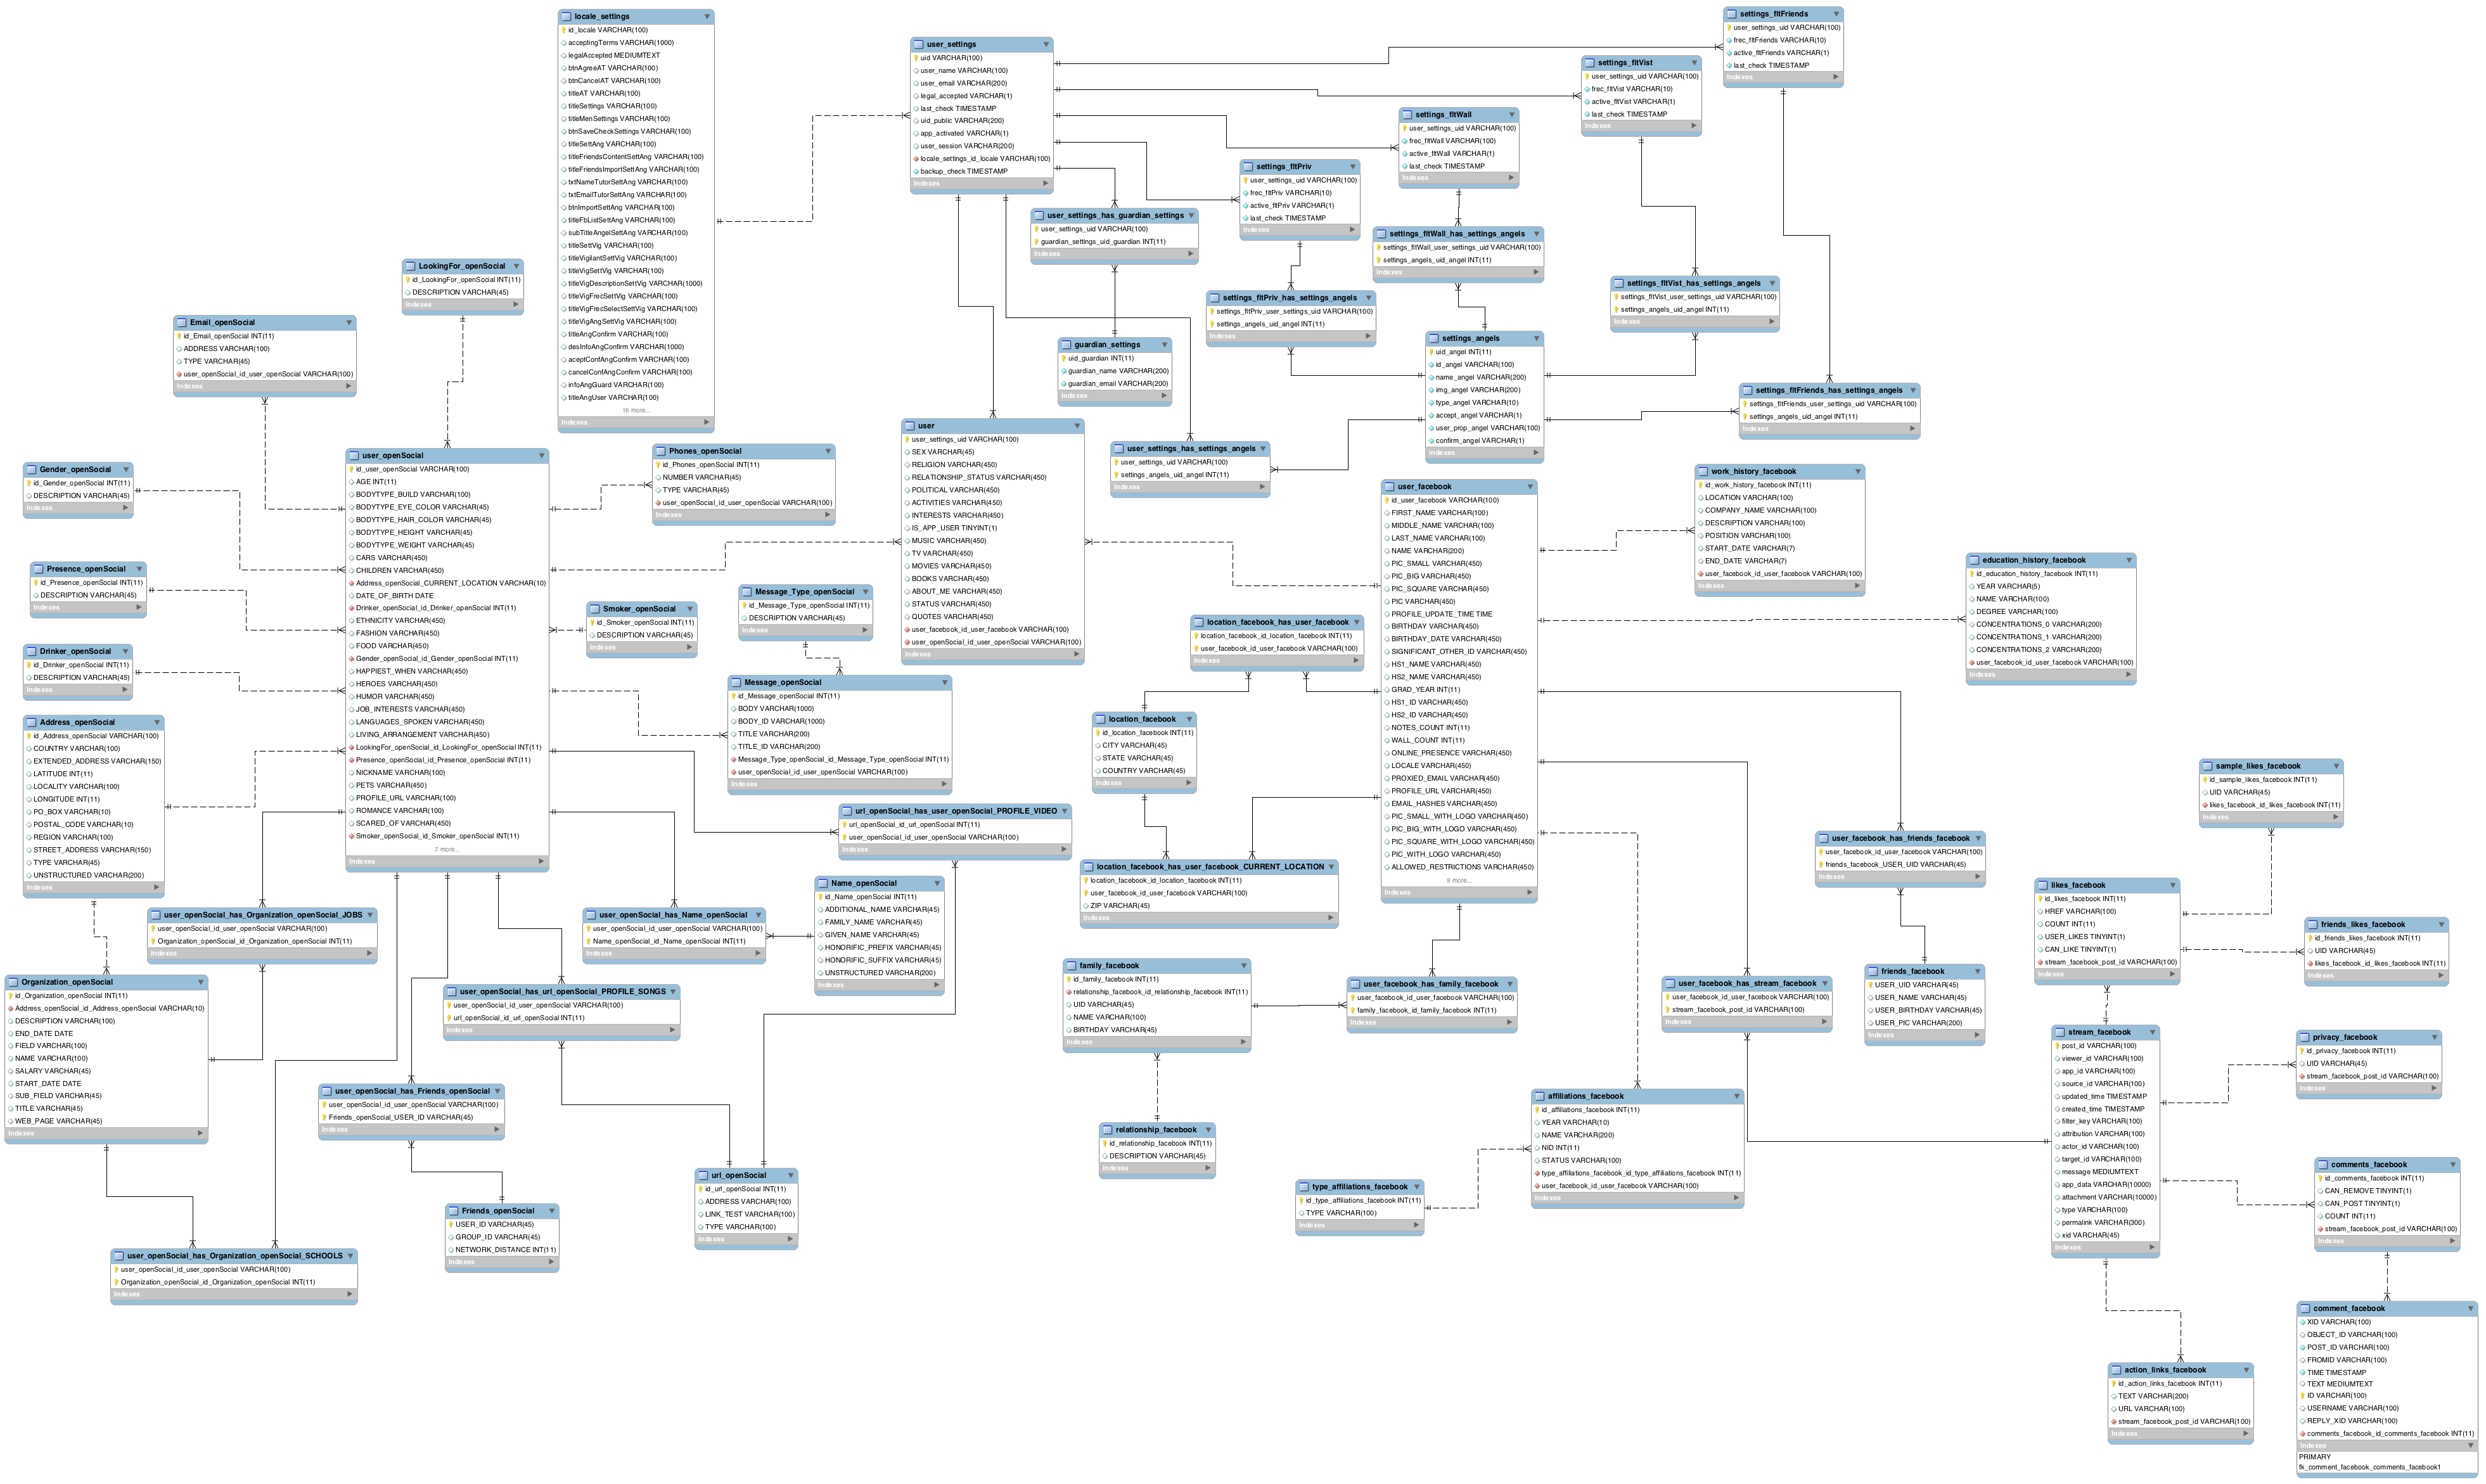
\includegraphics[width=17cm,height=19cm]{Figuras/lastModelSocialNetworkDB.png}
\end{center}
\caption{\label{ModeloER} Modelo Entidad-Relación de la base de datos de SNSAngelGuard}
\end{figure}
\bigskip
\par
La base de datos tiene tres estructuras bien definidas:
\begin{enumerate}
\item Módulo de configuración de SNSAngelGuard: En este módulo se especificarán las estructuras necesarias para la configuración de la aplicación. Contendrá estructuras para guardar los filtros\footnote[1]{Aplicaciones que analizarán la actividad social de un determinado usuario y generarán informes que serán enviados a sus ángeles.} que un usuario desee aplicar a su información, los ángeles\footnote[2]{Tutores a quienes van dirigidos los informes de la actividad social de un determinado usuario.} y la periodicidad con que éstos recibirán los informes generados por la aplicación.
\item Módulo propio de Facebook: Este módulo contendrá todas las estructuras necesarias para almacenar la información de un usuario que genera en Facebook y que será necesaria para el funcionamiento de la aplicación.
\item Módulo para otras Redes Sociales: Éste módulo contendrá las estructuras necesarias para almacenar información de otras redes sociales. Se diseñó utilizando el standar de Red Social proporcionado por OpenSocial y podrá ser adaptado a cualquier Red Social para la que se desee realizar un estudio determinado.
\end{enumerate}
\bigskip
\par
El desarrollo de ésta base de datos ha sido realizado íntegramente bajo el entorno MySQL versión 5. Para la administración, se ha utilizado el software MySQLAdmin bajo plataforma UNIX, la cual puede ser utilizada tanto en sistemas Linux, como en sistemas de la familia Macintosh.


\subsection{Módulo de comunicación con la base de datos: Interfaz RestFul}
Como se ha indicado anteriormente, el módulo de comunicación con la que el Módulo Servidor se comunicará con la base de datos, será implementado a través de Servicios Web. Para ello, se describirán las siguientes estructuras:
\begin{enumerate}
\item Módulo de Servicios Web: Será un proyecto web independiente que dará soporte a la base de datos. En él se definirán todas las estructuras necesarias para dar soporte a los servicios web que posteriormente se utilizarán en la aplicación SNSAngelGuard.
\item API propia RESTFUL: Se definirá una clase que contendrá todos los accesos a los servicios web definidos en el Módulo anterior. La razón por la que se definirá esta estructura es para que cualquier usuario, desde cualquier punto del planeta, pueda utilizar la base de datos mediante una llamada a un método remoto que le dará los datos que desee, sin tener que construir una estructura propia para el acceso a la base de datos ni tener que montar en su equipo la base de datos. Con ésta decisión se garantiza el acceso a cualquier usuario que tenga permisos para ello y la consistencia y persistencia de los datos que en ésta se almacenan, ya que ningún usuario tendrá una copia de la base de datos en su equipo, sino que trabajará remotamente con la base de datos que se defina a nivel global y cuyos parámetros de acceso serán comunicados al usuario que la quiera utilizar.
\end{enumerate}

\subsection{Módulo servidor}
El módulo servidor será la parte de la aplicación que se dedicará a procesar toda el negocio de la aplicación. Tendrá toda la responsabilidad de la aplicación y su funcionalidad. Sus objetivos serán los siguientes:
\begin{enumerate}
\item Controlar el acceso a la aplicación y gestionar la configuración de un usuario.
\item Gestionar los datos personales del usuario que se extraerán y que serán utilizados en la aplicación.
\item Analizar los datos extraídos por medio de filtros y elaborar informes.
\item Enviar los informes a los ángeles del usuario, quienes serán, en último término, los encargados de garantizar y supervisar la actividad social de un usuario en Facebook.
\end{enumerate}
\bigskip
\par
Este módulo además será el encargado de asumir las siguientes responsabilidades:
\begin{enumerate}
\item Garantizar el acceso único a la información de un usuario desde la propia aplicación.
\item Garantizar la privacidad de la información almacenada en la base de datos SocialNetwork, al igual que administrarla y gestionarla para garantizar la ejecución de los filtros definidos.
\item Analizar toda la actividad social de un usuario y comunicar cualquier anomalía definida en los filtros a sus ángeles.
\item Mantener en todo momento informado a los ángeles que se han configurado para un determinado usuario.
\item Garantizar la seguridad de la información que se envía desde la propia aplicación hasta servidores web externos a ella, tales como Gmail o Facebook.
\end{enumerate}
\bigskip
\par
Este módulo será diseñado y construido en su totalidad en el lenguaje de programación Java, combinando tanto el paradigma de Programación Orientada a Objetos, como la Programación Web en parte servidor, utilizando para ello las estructuras necesarias proporcionadas por dicho lenguaje de programación.
\subsection{Módulo cliente}
El módulo cliente será el encargado de la interfaz gráfica por el que el usuario realizará la configuración de la aplicación, seleccionando los ángeles que supervisarán su actividad social y los filtros que analizarán su información y enviarán informes de ello a dichos ángeles. Los objetivos de éste módulo serán los siguientes:
\begin{enumerate}
\item Mostrar al usuario una interfaz amigable y atractiva.
\item Integrar dicha interfaz en Facebook como una aplicación más que se ejecute desde el perfil de usuario.
\item Mostrar todos y cada uno de los amigos de Facebook para que puedan ser seleccionados por el usuario como sus ángeles.
\item Habilitar accesos desde el interfaz para poder seleccionar contactos desde cuentas de correo Gmail.
\item Habilitar las estructuras básicas para poder introducir manualmente un ángel, mediante cuadros de texto para su nombre y su dirección de correo.
\item Mostrar y controlar todos los filtros disponibles que puedan ser configurados por el usuario, mostrando además una pequeña descripción relativa a los mismos.
\end{enumerate}
\bigskip
\par
A parte de éstos objetivos, el módulo cliente se enfrentará a las siguientes responsabilidades:
\begin{enumerate}
\item Mostrar correctamente todas las estructuras necesarias para el correcto funcionamiento de la aplicación.
\item Llevar a cabo todas las validaciones de datos necesarias para que al almacenar la información de configuración, los datos estén preparados para ser procesados por el módulo servidor.
\item Controlar, en todo momento, que el usuario actual sea el único que puede acceder a su propia información de configuración.
\item Habilitar estructuras para el almacenado de la información.
\item Habilitar estructuras que informen visualmente al usuario sobre posibles errores o advertencias en el proceso de configuración. 
\item Habilitar estructuras visuales de ayuda que sirvan para aclarar posibles dudas a la hora de guardar la configuración.
\end{enumerate}
\bigskip
\par 
Todo este módulo será conformado por todas las herramientas web disponibles en la actualidad. Las principales que se han utilizado son las siguientes:
\begin{enumerate}
\item Lenguaje HTML\footnote[1]{HyperText Marckup Language, hace referencia al lenguaje de marcado predominante para la elaboración de páginas web, que se utiliza para describir y traducir la estructura y la información en forma de texto, así como complementar el texto con objetos tales como imágenes o contenido multimedia.}: Será el encargado de realizar toda la parte visual y el almacenado de la información subyacente en la arquitectura.
\item Lenguaje JavaScript\footnote[2]{Es un lenguaje de programación interpretado, que se ejecuta en la parte de cliente en una arquitectura común de Cliente-Servidor. Se utiliza implementado mediante el navegador web, permitiendo mejoras en la interfaz de usuario y en páginas web dinámicas, cuyo contenido puede variar.}: Será el encargado de realizar todas las validaciones necesarias anteriores al envío de la información y de controlar el contenido dinámico de la aplicación según las preferencias del usuario a la hora de configurar la aplicación.
\item Lenguaje JSON\footnote[3]{JavaScript Object Notation, es un formato ligero para el intercambio de datos. JSON es un subconjunto de la notación literal de objetos de JavaScript que no requiere el uso de XML.}: Realizará la tarea de intercambiar información entre el módulo cliente y el módulo servidor. También será el encargado de transferir información desde la base de datos al módulo servidor y viceversa.
\item AJAX\footnote[4]{Asynchronous JavaScript And XML, JavaScript anasíncrono y XML, es una técnica de desarrollo web para crear aplicaciones interactivas o RIA (Rich Internet Applications). Estas aplicaciones se ejecutan en el cliente, es decir, en el navegador de los usuarios mientras se mantiene la comunicación asíncrona con el servidor en segundo plano. De esta forma es posible realizar cambios sobre las páginas sin necesidad de recargarlas, lo que significa aumentar la interactividad, velocidad y usabilidad en las aplicaciones.}: Será el encargado de realizar la navegación entre paginas web pertenecientes al módulo cliente y realizar las transferencias de información entre pestañas integradas en una única página web.
\item jQuery\footnote[5]{jQuery es una biblioteca de JavaScript, creada inicialmente por John Resig, que permite simplificar la manera de interactuar con los documentos HTML, manipular el árbol DOM, manejar eventos, desarrollar animaciones y agregar interacción con la técnica AJAX a páginas web.}: Será el encargado del acceso a los elementos html de las páginas web y agrupar funcionalidad JavaScript, haciendo el código más rápido y legible.
\item JSP\footnote[6]{JavaServer Pages es una tecnología Java que permite generar contenido dinámico para web, en forma de documentos HTML, XML o de otro tipo, permitiendo la inclusión de código Java que se ejecutará directamente en servidor.}: Será el encargado de embeber las páginas html y controlar el flujo de ejecución con el servidor, realizando todas las validaciones y las transferencias de información de un módulo a otro.
\end{enumerate}

\subsection{Modulo Offline}
El Módulo Offline será el encargado de realizar los procesos de carga, validación y análisis de datos de forma automática. Se ejecutará una o varias veces al día, como tarea programada en el servidor, y realizará las siguientes acciones:
\begin{enumerate}
\item Obtener, de la base de datos SocialNetwork, la información relativa a todos los usuarios de la aplicación.
\item Por cada usuario realizará las siguientes acciones:
\begin{enumerate}
\item Descargará la nueva información que haya generado en Facebook, tal como nuevos comentarios en el muro o nuevas amistades.
\item Dependiendo de la periodicidad con que tenga configurados los filtros, realizará un análisis de la nueva información obtenida.
\item Tras realizar el análisis, informará a los ángeles los resultados obtenidos.
\item Actualizará en base de datos la fecha y la hora del momento en el que se ha realizado el proceso de actualización de la información.
\end{enumerate}
\end{enumerate}
\bigskip
\par 
Éste módulo será vital para mantener la base de datos actualizada con la última información del usuario y para realizar todas las tareas programadas por los filtros. Será desarrollado en su totalidad en Java y contendrá dos pequeños módulos:
\begin{enumerate}
\item Módulo Servidor: Éste módulo se ejecutará en el servidor web de aplicaciones mediante una conexión establecida por una tarea programada. Cuando le llega ésta llamada, pondrá en marcha todo el procedimiento descrito en el apartado anterior.
\item Tarea Programada: Dependerá del servidor o máquina física en el que se ejecute el servidor de aplicaciones. Se programará temporalmente una o varias veces diarias para poder realizar los backups de mantenimiento de la información. Será el desencadenante del proceso y sin él el Módulo Offline no se ejecutaría.
\end{enumerate} 
% Formato para un capítulo cualquiera

%Título del capítulo
\chapter{Base de Datos SocialNetwork} 

\section{Introducción}
Para la realización del proyecto SNSAngelGuard se ha requerido el diseño de una base de datos que persista todos los elementos necesarios para el análisis y el procesado de la información. Como se ha indicado en los capítulos anteriores, la base de datos se diseño para albergar datos no sólo de Facebook, sino también de otras redes sociales, como pueden ser Tuenti o Twitter, bajo el estándar de red social de Open Social.
\bigskip
\par
Además, posteriormente, se requirió de una estructura que pudiera controlar la ejecución de la aplicación SNSAngelGuard, enlazando el concepto de usuario de la aplicación con el usuario de una red social, por lo que, un usuario que ejecuta la aplicación debe tener un usuario válido en la red social en la que lo esté ejecutando. Esta estructura es la que almacena toda la información referente a la configuración del usuario en la aplicación, abarcando desde los ángeles que define, hasta la periodicidad con que se ejecutarán sus filtros.
\bigskip
\par
En el diseño de la base de datos se aprecian los siguientes módulos funcionales:
\begin{enumerate}
\item Módulo funcional de Configuración: Este módulo contendrá todas aquellas tablas necesarias para almacenar la configuración del usuario referente a filtros en ejecución, periodicidad de éstos y ángeles seleccionados para cada filtro. Esta información podrá cambiar cada vez que el usuario entre en la aplicación y guarde una información distinta a la que había originalmente.
\item Módulo funcional de Datos Comunes: Este módulo contendrá aquellas estructuras de información comunes a Facebook y OpenSocial reagrupadas, para dotar de mayor estabilidad a la base de datos reordenando aquella información que pueda ser simplificada en ambas redes.
\item Módulo funcional de OpenSocial: Este módulo contendrá todas aquellas tablas necesarias para guardar la información referente a OpenSocial. Contendrá funcionalmente las tablas para guardar la misma información que las estructuras definidas para almacenar información de Facebook. Aunque en éste desarrollo no se va a utilizar, se explicará el modelo de datos para sucesivos desarrollos. 
\item Módulo funcional de Facebook: Contendrá todas aquellas tablas necesarias para albergar información personal del usuario de Facebook que actualmente utiliza la aplicación. Se podrán guardar datos personales de cualquier tipo, desde datos personales hasta referencias a los circulo familiares a los que pertenece o enlaces a las fotografías que cuelga en su perfil.
\end{enumerate}
\bigskip
\par
Enumerados los diferentes bloques funcionales, pasaremos a definirlos formalmente en los siguientes apartados.

\section{Módulo funcional de Configuración}
Este módulo, como bien se ha especificado anteriormente, contendrá todas las tablas relacionadas con la configuración de la propia aplicación. Será un modelo sencillo en el que inicialmente se puede guardar la siguiente información:
\begin{enumerate}
\item Datos del usuario: Será la tabla maestra que controlará toda la aplicación. Todo usuario de la aplicación deberá tener un registro persistido en ésta tabla, aunque en el resto de tablas no contenga datos. En ella se almacenarán datos tales como su correo electrónico, el indicador de si la aplicación está activa, la fecha de la ultima actualización de datos, ..., etc.
\item Ángeles seleccionados: Será la tabla que almacene todos los datos de los ángeles que han sido definidos para controlar al usuario de la aplicación. Esta tabla estará relacionada con las tablas de filtros, siendo éstas últimas las que irán a buscar datos de los ángeles configurados en los filtros a la primera.
\item Filtros configurados: Actualmente existen cuatro filtros disponibles:
\begin{enumerate}
\item Filtro de control vocabulario ofensivo.
\item Filtro de control de amigos.
\item Filtro de control de privacidad.
\item Filtro de control de visitas.
\end{enumerate}
\end{enumerate}
Para todos ellos existirá una tabla en la que se almacenará si el filtro está activo y la frecuencia con la que se desea aplicar sobre la información. Cada tabla tendrá una relación con la tabla de ángeles en la que se especificará los ángeles que pertenecen a cada filtro.
\bigskip
\par 
Funcionalmente, el módulo ya está definido. Pasemos ahora a explicar detalladamente el modelo físico que se ha diseñado para tal fin.
\subsection{Tabla user\_settings}
Esta tabla albergará la información del usuario. Será la tabla maestra de la aplicación, por lo que todo usuario que pertenezca a la aplicación deberá tener un registro en ésta. Se relacionará con la tabla user en una relación 1 a 1, por lo que se cumple la anterior premisa, ya que ésta última contendrá datos maestros tanto de Facebook como de OpenSocial. Los campos de la tabla user\_settings son los mostrados en la tabla \ref{tabUserSettings}.
\begin{table}
\begin{center}

\begin{tabular}[c]{| l | l | p{60mm} |}\hline
\textbf{Campo}&\textbf{Tipo}&\textbf{Descripción} \\ \hline
uid & VARCHAR(100) & Contiene el identificador del usuario en la aplicación. Corresponderá al usuario de Facebook. \\ \hline
user\_name & VARCHAR(100) & Nombre del usuario \\ \hline
user\_email & VARCHAR(200) & Email del usuario \\ \hline
legal\_accepted & VARCHAR(1) & Indicador de aceptación del acuerdo legal por parte del usuario. \\ \hline
last\_check & TIMESTAMP & Fecha de la última ejecución de la aplicación cliente. \\ \hline
uid\_public & VARCHAR(200) & Identificador público del usuario. \\ \hline
app\_activated & VARCHAR(1) & Indica si la aplicación está activada o no. \\ \hline
user\_session & VARCHAR(200) & Token de sesión de Facebook para accesos offline. \\ \hline
locale\_settings\_id\_locale & VARCHAR(100) & Índice de la tabla locale\_settings que indica el idioma en el que se va a mostrar la aplicación. \\ \hline
bakup\_check & TIMESTAMP & Indica la última actualización de información del usuario. \\ \hline
\end{tabular}
\end{center}
\caption{Tabla user\_settings} \label{tabUserSettings}
\end{table}

\subsection{Tabla locale\_settings}
Esta tabla almacenará toda la información referente al idioma en que el usuario ejecuta la aplicación. Contendrá la información necesaria para poder traducir la aplicación(títulos de páginas, botones, ayuda, ..., etc.) al idioma en el que el usuario tenga configurado Facebook, es decir, si su perfil de dicha Red Social está en Castellano, la aplicación se mostrará en Castellano. Si por el contrario, estuviera en Inglés, la aplicación se mostraría en Inglés. Actualmente, la aplicación SNSAngelGuard cuenta con soporte para Castellano e Inglés. 
\bigskip
\par
Esta tabla estará relacionada mediante el campo locale\_settings\_id\_locale perteneciente a la tabla user\_settings. Éste campo contendrá el identificador del registro de la tabla locale\_settings a la cual hace referencia, obteniendo a partir de éste todos los recursos de idioma de la aplicación. La tabla \ref{tabLocaleSettings} muestra toda la información que contiene ésta estructura.

\begin{center}
\begin{longtable}{|l|l|p{60mm} |}

%Cabecera y primera hoja de la tabla
\caption{Tabla locale\_settings} \label{tabLocaleSettings}\\
\hline \multicolumn{1}{|l|}{\textbf{Campo}} & \multicolumn{1}{l|}{\textbf{Tipo}} & \multicolumn{1}{p{60mm} |}{\textbf{Descripción}} \\ 
\hline 
\endfirsthead

%Cabecera y resto de hojas de la tabla
\hline \multicolumn{1}{|l|}{\textbf{Campo}} & \multicolumn{1}{l|}{\textbf{Tipo}} & \multicolumn{1}{p{60mm}|}{\textbf{Descripción}} \\ \hline 
\endhead

\hline
id\_locale & VARCHAR(100) & Identificador único de la tabla. \\ \hline
acceptingTerms & VARCHAR(1000) & Cabecera del acuerdo legal. \\ \hline
legalAccepted & MEDIUMTEXT & Texto de aceptación de los términos de ejecución de la aplicación. \\ \hline
btnAgreeAT & VARCHAR(100) & Título del botón `Aceptar' de la página de Aceptación de Términos. \\ \hline
btnCancelAT & VARCHAR(100) & Título del botón `Cancelar' de la página de Aceptación de Términos. \\ \hline
titleAT & VARCHAR(100) & Título de la página de Aceptación de Términos. \\ \hline
titleSettings & VARCHAR(100) & Título de la página contenedora de la aplicación. \\ \hline
titleMenSettings & VARCHAR(100) & Título de las pestañas de la página contenedora. \\ \hline
btnSaveCheckSettings & VARCHAR(100) & Título del botón `Guardar' de la página de contenedora de la aplicación. \\ \hline
titleSettAng & VARCHAR(100) & Título principal de la página de la pestaña `Angeles' \\ \hline
titleFriendsContentSettAng & VARCHAR(100) & Título del frame de selección de ángeles de Facebook \\ \hline
titleFriendsImportSettAng & VARCHAR(100) & Títulos de los frams de selección de contactos de Google u otros contactos\\ \hline
txtNameTutorSettAng & VARCHAR(100) & Título para el nombre de un contacto del frame `Otros contactos'. \\ \hline
txtEmailTutorSettAng & VARCHAR(100) & Título para el email de un contacto del frame `Otros contactos'. \\ \hline
btnImportSettAng & VARCHAR(100) & Título del botón "Importar" contactos de Google. \\ \hline
titleFbListSettAng & VARCHAR(100) &  Contiene los nombres de las pestañas que visualizan los contactos de Facebook. \\ \hline
subTitleAngelSettAng & VARCHAR(100) &  Contiene los subtitulos que aparecen en cada contacto de Facebook. \\ \hline
titleSettVig & VARCHAR(100) & Título de la página de configuración de los vigilantes. \\ \hline
titleVigilantSettVig & VARCHAR(100) & Titulo del frame `Vigilantes' de la pestaña `Vigilantes'. \\ \hline
titleVigSettVig & VARCHAR(100) & Título de los filtros vigilantes disponibles.  \\ \hline
titleVigDescriptionSettVig & VARCHAR(100) &  Descripciones de cada vigilante. \\ \hline
titleVigFrecSettVig & VARCHAR(100) &  Título de la lista desplegable `Frecuencia'. \\ \hline
titleVigFrecSelectSettVig & VARCHAR(100) &  Valores disponibles de la lista desplegable `Frecuencia'. \\ \hline
titleVigAngSettVig & VARCHAR(100) & Titulo del frame `Angeles' de la pestaña `Vigilantes'. \\ \hline
titleAngConfirm & VARCHAR(100) &  Título del email de confirmación enviado a un ángel. \\ \hline
desInfoAngConfirm & VARCHAR(100) & Cuerpo del email de confirmación enviado a un ángel. \\ \hline
aceptConfAngConfirm & VARCHAR(100) &  Título del link de confirmación enviado en el email a un ángel. \\ \hline
cancelConfAngConfirm & VARCHAR(100) &  Título del link de cancelación enviado en el email a un ánge. \\ \hline
infoAngGuard & VARCHAR(100) &  Información acerca de la aplicación eviado en cada email. \\ \hline
titleAngUser & VARCHAR(100) &  Título de la página de información acerca del usuario que pide confirmación a un ángel. \\ \hline
nameUserAngUser & VARCHAR(100) & Título del nombre del usuario de Facebook. \\ \hline
btnCloseAngUser & VARCHAR(100) &  Título del botón `Cerrar' de la página de información de un usuario de Facebook. \\ \hline
titleGoogleCont & VARCHAR(100) &  Titulo de la página de importación de contactos de Google. \\ \hline
titleContGoogleCont & VARCHAR(100) &  Subtítulo de la página de importación de contactos de Google. \\ \hline
btnLogGoogleCont & VARCHAR(100) &  Título del botón de login en Google. \\ \hline
titleNameContactGoogleCont & VARCHAR(100) &  Nombre del contacto de Google.\\ \hline
titleEmailContactGoogleCont & VARCHAR(100) &  Email del contacto de Google. \\ \hline
btnAceptGoogleCont & VARCHAR(100) & Título del botón `Aceptar' de la página de importación de contactos de Google. \\ \hline
btnCancelGoogleCont & VARCHAR(100) & Título del botón `Cancelar' de la página de importación de contactos de Google. \\ \hline
helpMe & MEDIUMTEXT &  Contenido de la página de ayuda de la aplicación. \\ \hline
warnings & MEDIUMTEXT &  Contenido de los mensajes de aviso y errores que pueden producirse en la aplicación. \\ \hline
titleInformationMessage & VARCHAR(100) & Título para los mensajes de aviso y errores. \\ \hline
informationMessage & MEDIUMTEXT &  Contenido de las páginas de confirmación offline para los ángeles. \\ \hline
mailDelete & MEDIUMTEXT &  Contenido del email de eliminación de un ángel por parte de un usuario. \\ \hline
mailNotification & MEDIUMTEXT &  Contenido del email de notificación de actividad de un usuario hacia sus ángeles. \\ \hline
altContactsAngelsEd & MEDIUMTEXT &  Títulos para los botones de acción para otros contactos.\\ \hline 
titleVisitsFilterOptions & MEDIUMTEXT &  Títulos para las diferentes estadísticas utilizadas en el filtro de visitas.\\ \hline 

\end{longtable}
\end{center}

\subsection{Tabla settings\_angels}
Esta tabla contendrá la información de todos aquellos ángeles definidos para cada usuario. Estará relacionada con la tabla user\_settings con una relación N a N, en la que muchos usuarios podrán tener muchos ángeles. De cada ángel se obtiene la siguiente información:
\begin{enumerate}
\item Su identificador. En éste caso, corresponderá con su correo electrónico para el envío de notificaciones.
\item Su dirección de correo electrónico.
\item Su nombre.
\item El tipo de angel, es decir, si pertenece a Facebook, Google u otros contactos.
\item Si ha aceptado ser el ángel de algún usuario de la aplicación.
\item El usuario al que pertenece dentro de la aplicación.
\item La imagen del ángel. Si pertenece a Facebook, se almacenará su foto de perfil en el sistema. En otro caso, el sistema almacenará la imagen de perfil por defecto.
\end{enumerate}
\bigskip
\par
Toda la información anterior puede verse reflejada en la tabla \ref{tabSettingsAngels}.
\begin{table}
\begin{center}

\begin{tabular}[c]{| l | l | p{60mm} |}\hline
\textbf{Campo}&\textbf{Tipo}&\textbf{Descripción} \\ \hline
uid\_angel & INTEGER & Identificador único del ángel en la tabla. \\ \hline
id\_angel & VARCHAR(100) & Id del ángel, es decir, su email. \\ \hline
name\_angel & VARCHAR(200) & Nombre del ángel. \\ \hline
img\_angel & VARCHAR(200) & Imagen del ángel. \\ \hline
type\_angel & VARCHAR(10) & Tipo del ángel. \\ \hline
accept\_angel & VARCHAR(1) & Indica si el ángel ha aceptado seguir a un usuario o no. Se representará con el valor 1 en caso afirmativo y 0 en caso negativo. \\ \hline
user\_prop\_angel & VARCHAR(100) & Usuario de la aplicación propietario del ángel. \\ \hline
confirm\_angel & VARCHAR(1) & Indica si el ángel ha respondido a la solicitud. Se representará con el valor 1 en caso afirmativo y 0 en caso negativo. \\ \hline
\end{tabular}
\end{center}
\caption{Tabla settings\_angels} \label{tabSettingsAngels}
\end{table}

\subsection{Tabla settings\_fltWall}
Para guardar la configuración del filtro de control de lenguaje para un determinado usuario de la aplicación, se diseñó la tabla settings\_fltWall. Para cada usuario, se almacenará la siguiente información:
\begin{enumerate}
\item Frecuencia a la que se ejecutará el filtro de control de lenguaje. Este campo contendrá un valor entre el 0 y el 6 que indicará lo siguiente:
\begin{enumerate}
\item 0: El filtro se ejecutará diariamente.
\item 1: El filtro se ejecutará cada semana.
\item 2: El filtro se ejecutará cada dos semanas.
\item 3: El filtro se ejecutará mensualmente(valor por defecto).
\item 4: El filtro se ejecutará cada dos meses.
\item 5: El filtro se ejecutará cada seis meses.
\item 6: El filtro se ejecutará anualmente.
\end{enumerate}
\item Si se encuentra activo.
\item La fecha de la última vez que se ejecutó el filtro.
\end{enumerate}
\bigskip
\par
Esta tabla, además, estará relacionada N a N con la tabla settings\_angels, de la cual se obtendrán aquellos ángeles que estén configurados para este filtro, a los cuales se les enviará, cuando la frecuencia indique, los informes de notificación correspondientes a la ejecución del filtro.
\bigskip
\par
La estructura física de la tabla puede observarse en la tabla \ref{tabSettingsFltWall}.
\begin{table}
\begin{center}
\begin{tabular}[c]{| l | l | p{60mm} |}\hline
\textbf{Campo}&\textbf{Tipo}&\textbf{Descripción} \\ \hline
user\_settings\_uid & VARCHAR(1000) & Identificador único del usuario de la aplicación. \\ \hline
frec\_fltWall & VARCHAR(100) & Frecuencia a la que se ejecutará el filtro de control de lenguaje. \\ \hline
active\_fltWall & VARCHAR(1) & Indicador de actividad del filtro. El valor 1 indicará que el filtro se encuentra activo y el valor 0 indicará que no se encuentra activado. \\ \hline
last\_check & TIMESTAMP & Fecha de la última ejecución del filtro. \\ \hline
\end{tabular}
\end{center}
\caption{Tabla settings\_fltWall} \label{tabSettingsFltWall}
\end{table}

\subsection{Tabla settings\_fltFriends}
Esta tabla contendrá toda la información necesaria para la configuración del filtro de control de amistades. Para cada usuario se almacenará la siguiente información:
\begin{enumerate}
\item Frecuencia a la que se ejecutará el filtro. Como la tabla anterior, este campo almacenará los mismos códigos de frecuencia.
\item Si se encuentra activo.
\item La fecha de la última vez que se ejecutó el filtro.
\end{enumerate}
Para almacenar los ángeles con los que contará el filtro, se establece una relación N a N con la tabla settings\_angels, a los cuales se les enviará los informes de notificación de la ejecución del filtro.
\bigskip
\par
La estructura física de la tabla puede observarse en la tabla \ref{tabSettingsFltFriends}.
\begin{table}
\begin{center}
\begin{tabular}[c]{| l | l | p{60mm} |}\hline
\textbf{Campo}&\textbf{Tipo}&\textbf{Descripción} \\ \hline
user\_settings\_uid & VARCHAR(1000) & Identificador único del usuario de la aplicación. \\ \hline
frec\_fltFriends & VARCHAR(100) & Frecuencia a la que se ejecutará el filtro de control de amistades. \\ \hline
active\_fltFriends & VARCHAR(1) & Indicador de actividad del filtro. El valor 1 indicará que el filtro se encuentra activo y el valor 0 indicará que no se encuentra activado. \\ \hline
last\_check & TIMESTAMP & Fecha de la última ejecución del filtro. \\ \hline
\end{tabular}
\end{center}
\caption{Tabla settings\_fltFriends} \label{tabSettingsFltFriends}
\end{table}

\subsection{Tabla settings\_fltVist}
Esta tabla contendrá toda la información necesaria para la ejecución del filtro de visitas de un determinado usuario. Para cada uno de éstos se almacenará la siguiente información:
\begin{enumerate}
\item Frecuencia a la que se almacenará el filtro. Con el mismo código de valores que los filtros anteriores.
\item Si se encuentra activo para el usuario propietario del filtro.
\item La fecha de la última vez que se ejecutó el filtro.
\end{enumerate}
Para almacenar los ángeles con los que contará el filtro, se establece una relación N a N con la tabla settings\_angels, a los cuales se les enviará los informes de notificación de la ejecución del filtro.
\bigskip
\par
La estructura física de la tabla puede observarse en la tabla \ref{tabSettingsFltVist}.
\begin{table}
\begin{center}
\begin{tabular}[c]{| l | l | p{60mm} |}\hline
\textbf{Campo}&\textbf{Tipo}&\textbf{Descripción} \\ \hline
user\_settings\_uid & VARCHAR(1000) & Identificador único del usuario de la aplicación. \\ \hline
frec\_fltVist & VARCHAR(100) & Frecuencia a la que se ejecutará el filtro de control de visitas. \\ \hline
active\_fltVist & VARCHAR(1) & Indicador de actividad del filtro. El valor 1 indicará que el filtro se encuentra activo y el valor 0 indicará que no se encuentra activado. \\ \hline
last\_check & TIMESTAMP & Fecha de la última ejecución del filtro. \\ \hline
\end{tabular}
\end{center}
\caption{Tabla settings\_fltVist} \label{tabSettingsFltVist}
\end{table}

\subsection{Tabla settings\_fltPriv}
Esta tabla contendrá toda la información necesaria para la ejecución del filtro de privacidad de un determinado usuario. Para cada uno de éstos se almacenará la siguiente información:
\begin{enumerate}
\item Frecuencia a la que se almacenará el filtro. Con el mismo código de valores que los filtros anteriores.
\item Si se encuentra activo para el usuario propietario del filtro.
\item La fecha de la última vez que se ejecutó el filtro.
\end{enumerate}
Para almacenar los ángeles con los que contará el filtro, se establece una relación N a N con la tabla settings\_angels, a los cuales se les enviará los informes de notificación de la ejecución del filtro.
\bigskip
\par
La estructura física de la tabla puede observarse en la tabla \ref{tabSettingsFltPriv}.
\begin{table}
\begin{center}
\begin{tabular}[c]{| l | l | p{60mm} |}\hline
\textbf{Campo}&\textbf{Tipo}&\textbf{Descripción} \\ \hline
user\_settings\_uid & VARCHAR(1000) & Identificador único del usuario de la aplicación. \\ \hline
frec\_fltPriv & VARCHAR(100) & Frecuencia a la que se ejecutará el filtro de control de privacidad. \\ \hline
active\_fltPriv & VARCHAR(1) & Indicador de actividad del filtro. El valor 1 indicará que el filtro se encuentra activo y el valor 0 indicará que no se encuentra activado. \\ \hline
last\_check & TIMESTAMP & Fecha de la última ejecución del filtro. \\ \hline
\end{tabular}
\end{center}
\caption{Tabla settings\_fltPriv} \label{tabSettingsFltPriv}
\end{table}

\section{Módulo funcional de Datos Comunes}
En éste modulo se agrupará toda aquella información que pueda ser común entre las Redes Sociales a analizar, tales como Facebook y OpenSocial. Evidentemente, los datos más propensos a ser reagrupados serán aquellos que atañen directamente a la faceta personal del usuario, tales como sus datos personales, sus intereses, relaciones personales, estatus, citas sobre libros, etc. Por esta razón, se ha diseñado una tabla maestra denominada `user' que será la que agrupe todos estos datos.

\subsection{Tabla user}
Esta tabla será maestra, es decir, estará relacionada directamente con el nivel superior, es decir, con la tabla user\_settings y con las del nivel inferior, user\_facebook y user\_opensocial. Es evidente que un usuario de la aplicación debe tener una entrada en ésta tabla para que los datos sean consistentes. Los datos que contiene son de índole personal y estarán almacenados físicamente en la estructura mostrada en la tabla \ref{tabUser}.
\bigskip
\par
\begin{table}
\begin{center}
\begin{tabular}[c]{| l | l | p{60mm} |}\hline
\textbf{Campo}&\textbf{Tipo}&\textbf{Descripción} \\ \hline
user\_settings\_uid & VARCHAR(1000) & Identificador único del usuario de la aplicación. \\ \hline
SEX & VARCHAR(45) & Sexo del usuario de la aplicación. \\ \hline
RELIGION & VARCHAR(450) & Tendencias religiosas del usuario. \\ \hline
RELATIONSHIP\_STATUS & VARCHAR(450) & Estado sentimental. \\ \hline
POLITICAL & VARCHAR(450) & Tendencias politicas.\\ \hline
ACTIVITIES & VARCHAR(450) & Actividades que realiza el usuario. \\ \hline
INTERESTS & VARCHAR(450) & Intereses del usuario. \\ \hline
IS\_APP\_USER & TINYINT & Indicador del perfil activo dentro de la Red Social. \\ \hline
MUSIC & VARCHAR(450) & Tendencias musicales del usuario. \\ \hline
TV & VARCHAR(450) & Programas televisivos que sigue o ha seguido actualmente. \\ \hline
MOVIES & VARCHAR(450) & Películas favoritas. \\ \hline
BOOKS & VARCHAR(450) & Libros favoritos. \\ \hline
ABOUT\_ME & VARCHAR(450) & Descripción propia del usuario dentro de su perfil en la Red Social. \\ \hline
STATUS & VARCHAR(450) & Estatus actual del usuario. \\ \hline
QUOTES & VARCHAR(450) & Citas o frases famosas que definen a un usuario. \\ \hline
user\_facebook\_id\_user\_facebook & VARCHAR(100) & Identificador de su usuario en Facebook. \\ \hline
user\_openSocial\_id\_user\_openSocial & VARCHAR(100) & Identificador de su usuario en OpenSocial. \\ \hline
\end{tabular}
\end{center}
\caption{Tabla user} \label{tabUser}
\end{table}

\section{Módulo funcional de OpenSocial}
Aunque como se ha especificado anteriormente no se ha realizado funcionalidad alguna para la Red Social OpenSocial, si que se ha preparado la base de datos para un próximo desarrollo sobre dicha Red Social que conlleve el análisis y estudio de los datos que se puedan generar. Para ello, se pasará a describir las estructuras físicas diseñadas para ser utilizadas a corto-medio plazo.

\subsection{Tabla user\_openSocial}
Es la tabla maestra de los datos de OpenSocial. Como se ha comentado anteriormente, desciende de la tabla de datos comunes \textbf{user}. En ella se centrarán todas las relaciones de datos e irán gestionadas desde esta tabla. Estas relaciones serán las siguientes:
\begin{enumerate}
\item Sus números de teléfono irán gestionados siguiendo una relación 1 a N con la tabla \textbf{Phones\_openSocial}.
\item Si es fumador, la tabla almacenará un código que será una entrada a la tabla maestra \textbf{Smoker\_openSocial}.
\item Sus preferencias en cuanto a tendencias sociales seguirán una relación 1 a N con la tabla \textbf{LookingFor\_openSocial}.
\item Todas sus direcciones de email se almacenarán, mediante una relación 1 a N, con la tabla \textbf{Email\_openSocial}.
\item Su sexo irá descrito mediante un codigo que referenciará una entrada a la tabla maestra \textbf{Gender\_openSocial}.
\item Su disponibilidad en OpenSocial irá descrita mediante un código que referenciará una entrada a la tabla maestra \textbf{Presence\_openSocial}.
\item Su grado de alcoholismo irá descrita mediante un código que referenciará una entrada a la tabla maestra \textbf{Drinker\_openSocial}.
\item Sus direcciones particulares seguirán una relación 1 a N con la tabla \textbf{Address\_ openSocial} que a su vez estará relacionada con la tabla \textbf{Organization\_ openSocial}, la cual será capaz de almacenar los lugares de trabajo o sitios donde haya estudiado mediante relaciones N a N.
\item Sus amigos dentro de OpenSocial serán almacenados, mediante una relación N a N, con la tabla \textbf{Friends\_openSocial}.
\item Las URLs sobre videos, clips de audio o páginas de interés serán almacenados, mediante una relación N a N, con la tabla \textbf{url\_openSocial}.
\item Los diferentes nombres o apodos que el usuario vaya utilizando a lo largo de su ciclo de vida en OpenSocial se almacenarán, mediante una relación N a N, con la tabla \textbf{Name\_openSocial}.
\item Los mensajes de muro que el usuario recibe en su perfil de OpenSocial se almacenarán, mediante una relación 1 a N, en la tabla \textbf{Message\_openSocial}.
\end{enumerate}


Su estructura física está representada en la tabla \ref{tabUserOpenSocial}.

\begin{center}
\begin{longtable}{|p{70mm} |l|p{60mm} |}

%Cabecera y primera hoja de la tabla
\caption{Tabla user\_openSocial} \label{tabUserOpenSocial}\\
\hline \multicolumn{1}{|l|}{\textbf{Campo}} & \multicolumn{1}{l|}{\textbf{Tipo}} & \multicolumn{1}{p{60mm} |}{\textbf{Descripción}} \\ 
\hline 
\endfirsthead

%Cabecera y resto de hojas de la tabla
\hline \multicolumn{1}{|l|}{\textbf{Campo}} & \multicolumn{1}{l|}{\textbf{Tipo}} & \multicolumn{1}{p{60mm}|}{\textbf{Descripción}} \\ \hline 
\endhead

\hline
id\_user\_openSocial & VARCHAR(100) & Identificador único de la tabla. \\ \hline
AGE & INTEGER & Edad del usuario. \\ \hline
BODYTYPE\_BUILD & VARCHAR(100)  & Complexión del usuario. \\ \hline
BODYTYPE\_EYE\_COLOR & VARCHAR(45) & Color de ojos. \\ \hline
BODYTYPE\_HAIR\_COLOR & VARCHAR(45) & Color de pelo. \\ \hline
BODYTYPE\_HEIGHT & VARCHAR(45) & Altura. \\ \hline
BODYTYPE\_WEIGHT & VARCHAR(45) & Peso. \\ \hline
CARS & VARCHAR(450) & Tendencias sobre coches. \\ \hline
CHILDREN & VARCHAR(450) & Hijos del usuario. \\ \hline
Address\_openSocial\_CURRENT\_ LOCATION & VARCHAR(10) & Dirección actual. \\ \hline
DATE\_OF\_BIRTH & DATE & Fecha de nacimiento. \\ \hline
Drinker\_openSocial\_id\_Drinker\_ openSocial & INTEGER & Grado de alcoholismo. \\ \hline
ETHNICITY & VARCHAR(450) & Raza étnica. \\ \hline
FASHION & VARCHAR(450) & Tendencias sobre moda. \\ \hline
FOOD & VARCHAR(450) & Tendencias gastronómicas. \\ \hline
Gender\_openSocial\_id\_Gender\_ openSocial & INTEGER &  Sexo del usuario. \\ \hline
HAPPIEST\_WHEN & VARCHAR(450) &  Actividades favoritas. \\ \hline
HEROES & VARCHAR(450) & Heroes. \\ \hline
HUMOR & VARCHAR(450) & Tendencias humorísticas. \\ \hline
JOB\_INTERESTS & VARCHAR(450) & Actividad laboral.  \\ \hline
LANGUAGES\_SPOKEN & VARCHAR(450) &  Idiomas hablados por el usuario. \\ \hline
LIVING\_ARRANGEMENT & VARCHAR(450) &  Alojamiento. \\ \hline
LookingFor\_openSocial\_id\_Looking For\_openSocial & INTEGER &  Relaciones sociales sobre las que está interesado. \\ \hline
Presence\_openSocial\_id\_Presence\_ openSocial & INTEGER & Presencia actual en la red. \\ \hline
NICKNAME & VARCHAR(100) &  Apodo. \\ \hline
PETS & VARCHAR(450) & Mascotas. \\ \hline
PROFILE\_URL & VARCHAR(100) &  URL de la foto de perfil del usuario. \\ \hline
ROMANCE & VARCHAR(100) &  Relación actual. \\ \hline
SCARED\_OF & VARCHAR(450) &  Miedos o temores. \\ \hline
Smoker\_openSocial\_id\_Smoker\_ openSocial & INTEGER &  Fumador. \\ \hline
SPORTS & VARCHAR(450) & Actividades deportivas del usuario. \\ \hline
TAGS & VARCHAR(450) &  Etiquetas asociadas al usuario. \\ \hline
THUMBNAIL\_URL & VARCHAR(100) &  URL a la imagen thumbnail del usuario. \\ \hline
TIME\_ZONE & DATE &  Franja horaria en la que se encuentra el usuario. \\ \hline
TURNS\_OFFS & VARCHAR(450) &  Tendencias que desagradan al usuario. \\ \hline
TURNS\_ONS & VARCHAR(450) &  Tendencias que sorprenden al usuario.\\ \hline
URLS & VARCHAR(450) &  URLs de interes del usuario. \\ \hline

\end{longtable}
\end{center}

\subsection{Tabla Phones\_openSocial}
Como se ha especificado anteriormente, será la tabla que contenga todos los números de teléfono del usuario. Conformará una relación 1 a N con la tabla \textbf{user\_openSocial}, ya que un usuario podrá tener N números de teléfono. Su estructura física estará representada en la tabla \ref{tabPhonesOpenSocial}.
\bigskip
\par
\begin{table}[h]
\begin{center}
\begin{tabular}{| l | l | p{60mm} |}\hline
\textbf{Campo}&\textbf{Tipo}&\textbf{Descripción} \\ \hline
id\_Phones\_openSocial & INTEGER & Identificador único de la tabla. \\ \hline
NUMBER & VARCHAR(45) & Numero de teléfono asociado al usuario. \\ \hline
TYPE & VARCHAR(45) & Tipo de teléfono( fijo, móvil, etc.). \\ \hline
user\_openSocial\_id\_user\_openSocial & VARCHAR(100) & Identificador de su usuario en OpenSocial. \\ \hline
\end{tabular}
\end{center}
\caption{Tabla Phones\_openSocial} \label{tabPhonesOpenSocial}
\end{table}

\subsection{Tabla Smoker\_openSocial}
Esta tabla contendrá todos los posibles valores para describir el grado de afición al tabaco por parte de un usuario. Será una tabla maestra que irá referenciada a la tabla \textbf{user\_openSocial} mediante un codigo de entrada que podrá representar los siguientes valores:
\begin{enumerate}
\item Valor \textbf{vacío}: Indicará que el usuario no ha definido esta característica en su perfil.
\item Valor \textbf{HEAVILY}: Indica que es fumador en exceso.
\item Valor \textbf{NO}: Indica que el usuario no es fumador.
\item Valor \textbf{OCCASIONALLY}: Indica que el usuario no es fumador pero puede fumar ocasionalmente.
\item Valor \textbf{QUIT}: Indica que el usuario era fumador pero actualmente lo ha dejado.
\item Valor \textbf{QUITTING}: Indica que el usuario está dejando de fumar.
\item Valor \textbf{REGULARLY}: Indica que el usuario fuma de forma regular.
\item Valor \textbf{SOCIALLY}: Indica que el usuario fuma unicamente en reuniones sociales.
\item Valor \textbf{YES}: Indica que el usuario es fumador.
\end{enumerate}
\bigskip
\par
La tabla \ref{tabSmokerOpenSocial} mostrará su organización física.
\bigskip
\par
\begin{table}[h]
\begin{center}
\begin{tabular}{| l | l | p{60mm} |}\hline
\textbf{Campo}&\textbf{Tipo}&\textbf{Descripción} \\ \hline
id\_Smoker\_openSocial & INTEGER & Identificador único de la tabla. \\ \hline
DESCRIPTION & VARCHAR(45) & Descripción para cada uno de los valores anteriores. \\ \hline
\end{tabular}
\end{center}
\caption{Tabla Smoker\_openSocial} \label{tabSmokerOpenSocial}
\end{table}

\subsection{Tabla LookingFor\_openSocial}
Esta tabla contendrá todos los valores posibles que se encuadran en la búsqueda de actividades o perfiles sociales que el usuario busca para poder relacionarse. Al igual que la tabla \textbf{Smoker\_openSocial}, será una tabla maestra cuyos valores son los siguientes:
\begin{enumerate}
\item Valor \textbf{vacío}: Indicará que el usuario no ha definido esta característica en su perfil.
\item Valor \textbf{ACTIVITY\_PARTNERS}: Compañeros de actividad que comparten los mismos intereses sociales.
\item Valor \textbf{DATING}: Amigos para un servicio a corto plazo.
\item Valor \textbf{FRIENDS}: Amigos permanentes.
\item Valor \textbf{NETWORKING}: Compañeros de actividad en internet, como jugadores en red o compañeros de trabajo.
\item Valor \textbf{RANDOM}: Aleatorio, indiferente.
\item Valor \textbf{RELATIONSHIP}: Una relación, ya sea familiar o un vínculo sentimental.
\end{enumerate}
\bigskip
\par
La tabla \ref{tabLookingForOpenSocial} mostrará su estructura física dentro del sistema.
\bigskip
\par
\begin{table}[h]
\begin{center}
\begin{tabular}{| l | l | p{60mm} |}\hline
\textbf{Campo}&\textbf{Tipo}&\textbf{Descripción} \\ \hline
id\_LookingFor\_openSocial & INTEGER & Identificador único de la tabla. \\ \hline
DESCRIPTION & VARCHAR(45) & Descripción para cada uno de los valores anteriores. \\ \hline
\end{tabular}
\end{center}
\caption{Tabla LookingFor\_openSocial} \label{tabLookingForOpenSocial}
\end{table}

\subsection{Tabla Email\_openSocial}
Esta tabla contendrá todas las direcciones de correo electrónico que hayan sido introducidas por el usuario de OpenSocial en su perfil. Estará relacionada 1 a N con la tabla \textbf{user\_openSocial} y su estructura física se muestra en la tabla \ref{tabEmailOpenSocial}.
\bigskip
\par
\begin{table}[h]
\begin{center}
\begin{tabular}{| l | l | p{60mm} |}\hline
\textbf{Campo}&\textbf{Tipo}&\textbf{Descripción} \\ \hline
id\_Email\_openSocial & INTEGER & Identificador único de la tabla. \\ \hline
ADDRESS & VARCHAR(100) & Dirección de correo electrónico. \\ \hline
TYPE & VARCHAR(45) & Descripción del tipo de cuenta de correo electrónico. \\ \hline
user\_openSocial\_id\_user\_openSocial & VARCHAR(100) & Identificador de su usuario en OpenSocial. \\ \hline
\end{tabular}
\end{center}
\caption{Tabla Email\_openSocial} \label{tabEmailOpenSocial}
\end{table}

\subsection{Tabla Gender\_openSocial}
Será una tabla maestra que definirá el sexo del usuario en OpenSocial. Sus valores serán los siguientes:
\begin{enumerate}
\item Valor \textbf{vacío}: Indicará que el usuario no ha definido esta característica en su perfil.
\item Valor \textbf{MALE}: Sexo masculino.
\item Valor \textbf{FEMALE}: Sexo femenino.
\end{enumerate}
\bigskip
\par
La tabla \ref{tabGenderOpenSocial} mostrará su organización física.
\bigskip
\par
\begin{table}[h]
\begin{center}
\begin{tabular}{| l | l | p{60mm} |}\hline
\textbf{Campo}&\textbf{Tipo}&\textbf{Descripción} \\ \hline
id\_Gender\_openSocial & INTEGER & Identificador único de la tabla. \\ \hline
DESCRIPTION & VARCHAR(45) & Descripción para cada uno de los valores anteriores. \\ \hline
\end{tabular}
\end{center}
\caption{Tabla Gender\_openSocial} \label{tabGenderOpenSocial}
\end{table}

\subsection{Tabla Presence\_openSocial}
Esta tabla indicará el estado actual del usuario en OpenSocial. Será también una tabla maestra que contendrá valores fijos que serán referenciados desde la tabla \textbf{user\_openSocial}. Sus valores serán los siguientes:
\begin{enumerate}
\item Valor \textbf{vacío}: Indicará que el usuario no ha definido esta característica en su perfil.
\item Valor \textbf{AWAY}: El usuario está conectado pero se encuentra ausente.
\item Valor \textbf{CHAT}: El usuario se encuentra manteniendo una conversación por chat.
\item Valor \textbf{DND}: Son las siglas `Do Not Disturb', por lo que el usuario estará en estado `No disponible'.
\item Valor \textbf{OFFLINE}: El usuario se encuentra desconectado actualmente.
\item Valor \textbf{ONLINE}: El usuario se encuentra conectado actualmente.
\item Valor \textbf{XA}: Son las siglas `Extended Away', por lo que el usuario se encontrará en un rango temporal elevado de inactividad aunque se encuentre conectado.
\end{enumerate}
\bigskip
\par
La tabla \ref{tabPresenceOpenSocial} mostrará su organización física.
\bigskip
\par
\begin{table}[h]
\begin{center}
\begin{tabular}{| l | l | p{60mm} |}\hline
\textbf{Campo}&\textbf{Tipo}&\textbf{Descripción} \\ \hline
id\_Presence\_openSocial & INTEGER & Identificador único de la tabla. \\ \hline
DESCRIPTION & VARCHAR(45) & Descripción para cada uno de los valores anteriores. \\ \hline
\end{tabular}
\end{center}
\caption{Tabla Presence\_openSocial} \label{tabPresenceOpenSocial}
\end{table}

\subsection{Tabla Drinker\_openSocial}
Esta tabla contendrá todos los posibles valores que existen en OpenSocial para describir el posible grado de alcoholimo del usuario. Al igual que todas las tablas de valores anteriores, será una tabla maestra referenciada desde la tabla \textbf{user\_openSocial}. Los valores definidos para ella serán los siguientes:
\begin{enumerate}
\item Valor \textbf{vacío}: Indicará que el usuario no ha definido esta característica en su perfil.
\item Valor \textbf{NO}: Indica que el usuario no bebe.
\item Valor \textbf{OCCASIONALLY}: Indica que el usuario no es bebedor pero puede beber ocasionalmente.
\item Valor \textbf{QUIT}: Indica que el usuario era bebedor pero actualmente lo ha dejado.
\item Valor \textbf{QUITTING}: Indica que el usuario está dejando de beber.
\item Valor \textbf{REGULARLY}: Indica que el usuario bebe de forma regular.
\item Valor \textbf{SOCIALLY}: Indica que el usuario bebe unicamente en reuniones sociales.
\item Valor \textbf{YES}: Indica que el usuario es bebedor.
\item Valor \textbf{HEAVILY}: Indica que es bebedor en exceso.
\end{enumerate}
\bigskip
\par
La tabla \ref{tabDrinkerOpenSocial} mostrará su organización física.
\bigskip
\par
\begin{table}[h]
\begin{center}
\begin{tabular}{| l | l | p{60mm} |}\hline
\textbf{Campo}&\textbf{Tipo}&\textbf{Descripción} \\ \hline
id\_Drinker\_openSocial & INTEGER & Identificador único de la tabla. \\ \hline
DESCRIPTION & VARCHAR(45) & Descripción para cada uno de los valores anteriores. \\ \hline
\end{tabular}
\end{center}
\caption{Tabla Drinker\_openSocial} \label{tabDrinkerOpenSocial}
\end{table}

\subsection{Tablas de direcciones Address\_openSocial y Organization\_ openSocial}
Estas tablas serán las encargadas de almacenar cualquier dirección de interés relacionada con el usuario. 
\bigskip
\par
La tabla \textbf{Address\_openSocial} almacenará toda la información respecto a la dirección física de un usuario tal como la dirección donde vive o su lugar de trabajo. Estará relacionada con la tabla \textbf{user\_openSocial} mediante una relación 1 a N y su estructura física puede verse en la tabla \ref{tabAddressOpenSocial}.
\bigskip
\par
\begin{table}[h]
\begin{center}
\begin{tabular}{| l | l | p{60mm} |}\hline
\textbf{Campo}&\textbf{Tipo}&\textbf{Descripción} \\ \hline
id\_Address\_openSocial & VARCHAR(100) & Identificador único de la tabla. \\ \hline
COUNTRY & VARCHAR(100) & País. \\ \hline
EXTENDED\_ADDRESS & VARCHAR(150) &  Dirección postal para direcciones largas.\\ \hline
LATITUDE & INTEGER & Linea de latitud del lugar. \\ \hline
LOCALITY & VARCHAR(100) & Localidad. \\ \hline
LONGITUDE & INTEGER &  Linea de longitud del lugar. \\ \hline
PO\_BOX & VARCHAR(10) &  Apartado postal. \\ \hline
POSTAL\_CODE & VARCHAR(10) &  Codigo postal. \\ \hline
REGION & VARCHAR(100) & Región del lugar. \\ \hline
STREET\_ADDRESS & VARCHAR(150) & Dirección postal.  \\ \hline
TYPE & VARCHAR(45) &  Tipo de la dirección( casa, trabajo, etc.). \\ \hline
UNSTRUCTURED & VARCHAR(200) & Si no se ha guardado la información estructuradamente, este campo almacenará toda la información de la dirección del usuario. \\ \hline
\end{tabular}
\end{center}
\caption{Tabla Address\_openSocial} \label{tabAddressOpenSocial}
\end{table}
\bigskip
\par
La tabla \textbf{Organization\_openSocial} será una extensión de la tabla anterior. Esta tabla almacenará información sobre lugares de trabajo o lugares de estudio del usuario y utilizará la tabla anterior para almacenar su dirección, mientras que la tabla Organization\_openSocial almacenará datos propios del trabajo. Estará relacionada con la tabla \textbf{user\_openSocial} de dos maneras:
\begin{enumerate}
\item Utilizará una relacion N a N para almacenar todos los trabajos del usuario.
\item Utilizará también otra relación N a N para almacenar su historial académico sobre los lugares donde estudió.
\end{enumerate}
\bigskip
\par
Su estructura física podrá verse en la tabla \ref{tabOrganizationOpenSocial}.
\bigskip
\par
\begin{table}[h]
\begin{center}
\begin{tabular}{| p{65mm} | l | p{60mm} |}\hline
\textbf{Campo}&\textbf{Tipo}&\textbf{Descripción} \\ \hline
id\_Organization\_openSocial & INTEGER & Identificador único de la tabla. \\ \hline
Address\_openSocial\_id\_Address\_ openSocial & VARCHAR(10) & Referencia a la entrada en la tabla Address\_openSocial en la que está almacenada su dirección. \\ \hline
DESCRIPTION & VARCHAR(100) & Descripción del trabajo. \\ \hline
END\_DATE & DATE &  Fecha fin del trabajo.\\ \hline
FIELD & VARCHAR(100) & Mercado de trabajo. \\ \hline
NAME & VARCHAR(100) &  Nombre de la empresa. \\ \hline
SALARY & VARCHAR(45) &  Salario. \\ \hline
START\_DATE & DATE &  Fecha de inicio del trabajo. \\ \hline
SUB\_FIELD & VARCHAR(45) & Campo del mercado de trabajo. \\ \hline
TITLE & VARCHAR(45) & Puesto de trabajo que ostenta. \\ \hline
WEB\_PAGE & VARCHAR(45) & Página web de la empresa. \\ \hline
\end{tabular}
\end{center}
\caption{Tabla Organization\_openSocial} \label{tabOrganizationOpenSocial}
\end{table}

\subsection{Tabla Friends\_openSocial}
Esta tabla contendrá todos los amigos del usuario en OpenSocial. Estará relacionada N a N con la tabla \textbf{user\_openSocial} ya que un amigo puede tener N amigos y, además, coincidir con varios amigos de otro usuario de OpenSocial con M amigos. Su estructura física se muestra en la tabla \ref{tabFriendsOpenSocial}.
\bigskip
\par
\begin{table}[h]
\begin{center}
\begin{tabular}{| l | l | p{60mm} |}\hline
\textbf{Campo}&\textbf{Tipo}&\textbf{Descripción} \\ \hline
USER\_UID & VARCHAR(45) & Identificador único del amigo en OpenSocial. \\ \hline
GROUP\_ID & VARCHAR(45) & Grupo de amigos al que pertenece. \\ \hline
NETWORK\_DISTANCE & INTEGER & Parámetro asignado por OpenSocial. Si el contacto pertenece a un grupo de amigos con los que tiene contacto frecuente, se le asignará una distancia menor, siendo mayor en caso contrario. \\ \hline
\end{tabular}
\end{center}
\caption{Tabla Friends\_openSocial} \label{tabFriendsOpenSocial}
\end{table}

\subsection{Tabla url\_openSocial}
Esta tabla contendrá todos los posibles links que sean de interés para el usuario. Todos aquellos enlaces de video o de cualquier otro tipo deberán tener una entrada en ésta tabla. Estará relacionada con la tabla \textbf{user\_openSocial} de las siguientes maneras:
\begin{enumerate}
\item Una relación N a N para guardar todos los enlaces con referencias a videos.
\item Una relación N a N para guardar todos los enlaces con refecencias a canciones de música.
\end{enumerate}
\bigskip
\par
La tabla \ref{tabUrlOpenSocial} mostrará su estructura física.
\begin{table}[h]
\begin{center}
\begin{tabular}{| l | l | p{60mm} |}\hline
\textbf{Campo}&\textbf{Tipo}&\textbf{Descripción} \\ \hline
id\_url\_openSocial & INTEGER & Identificador único de la tabla. \\ \hline
ADDRESS & VARCHAR(100) & Dirección url. \\ \hline
LINK\_TEST & VARCHAR(100) & Dirección url test en caso de error. \\ \hline
TYPE & VARCHAR(100) & Tipo de url. \\ \hline
\end{tabular}
\end{center}
\caption{Tabla url\_openSocial} \label{tabUrlOpenSocial}
\end{table}

\subsection{Tabla Name\_openSocial}
Esta tabla contendrá todo el historial de nombres u apodos que el usuario vaya usando en su perfil de OpenSocial. Estará relacionada con la tabla \textbf{user\_openSocial} con una relación N a N. Su estructura física será la mostrada en la tabla \ref{tabNameOpenSocial}.
\bigskip
\par
\begin{table}
\begin{center}
\begin{tabular}{| l | l | p{60mm} |}\hline
\textbf{Campo}&\textbf{Tipo}&\textbf{Descripción} \\ \hline
id\_Name\_openSocial & INTEGER & Identificador único de la tabla. \\ \hline
ADDITIONAL\_NAME & VARCHAR(45) & Nombre adicional del usuario. \\ \hline
FAMILY\_NAME & VARCHAR(45) & Nombre con el que se conoce familiarmente al usuario. \\ \hline
GIVEN\_NAME & VARCHAR(45) & Apodo del usuario. \\ \hline
HONORIFIC\_PREFIX & VARCHAR(45) & Prefijo honorífico del usuario. \\ \hline
HONORIFIC\_SUFFIX & VARCHAR(45) & Sufijo honorífico del usuario. \\ \hline
UNSTRUCTURED & VARCHAR(45) & Campo que almacena toda la información sin estructurar. \\ \hline
\end{tabular}
\end{center}
\caption{Tabla Name\_openSocial} \label{tabNameOpenSocial}
\end{table}

\subsection{Tabla Message\_openSocial}
Esta tabla contendrá información sobre cualquier mensaje que el usuario reciba en su perfil de OpenSocial. La tabla \textbf{Message\_Type\_openSocial} determina, mediante un conjunto de valores referenciados por la tabla \textbf{Message\_openSocial}, qué tipo de mensaje se está almacenando. Sus posibles valores serán los siguientes:
\begin{enumerate}
\item Valor \textbf{vacío}: Indicará que el tipo de mensaje no está definido.
\item Valor \textbf{EMAIL}: Indica que el mensaje es un email.
\item Valor \textbf{NOTIFICATION}: Indica que el mensaje es una notificación de alguna aplicación.
\item Valor \textbf{PRIVATE\_MESSAGE}: Indica que el mensaje es un mensaje privado.
\item Valor \textbf{PUBLIC\_MESSAGE}: Indica que el mensaje es un mensaje público, como puede ser un mensaje en el muro.
\end{enumerate}
\bigskip
\par
Su estructura física puede observarse en la tabla \ref{tabMessageTypeOpenSocial}.
\begin{table}[h]
\begin{center}
\begin{tabular}{| l | l | p{60mm} |}\hline
\textbf{Campo}&\textbf{Tipo}&\textbf{Descripción} \\ \hline
id\_Message\_Type\_openSocial & INTEGER & Identificador único de la tabla. \\ \hline
DESCRIPTION & VARCHAR(45) & Descripción para cada uno de los valores anteriores. \\ \hline
\end{tabular}
\end{center}
\caption{Tabla Message\_Type\_openSocial} \label{tabMessageTypeOpenSocial}
\end{table}
\bigskip
\par
Tras haber definido el tipo de mensaje, la tabla \textbf{Message\_openSocial} estará relacionada con la tabla \textbf{user\_openSocial} con una relación 1 a N. Su estructura física puede observarse en la tabla \ref{tabMessageOpenSocial}.
\bigskip
\par
\begin{table}[h]
\begin{center}
\begin{tabular}{| p{65mm}  | l | p{60mm} |}\hline
\textbf{Campo}&\textbf{Tipo}&\textbf{Descripción} \\ \hline
id\_Message\_openSocial & INTEGER & Identificador único de la tabla. \\ \hline
BODY & VARCHAR(1000) & Cuerpo del mensaje. \\ \hline
BODY\_ID & VARCHAR(1000) & Cuerpo del mensaje codificado mediante templates. \\ \hline
TITLE & VARCHAR(200) & Título del mensaje. \\ \hline
TITLE\_ID & VARCHAR(200) & Título del mensaje codificado mediante templates. \\ \hline
Message\_Type\_openSocial\_id\_ Message\_Type\_openSocial & INTEGER & Tipo del mensaje. \\ \hline
user\_openSocial\_id\_user\_ openSocial & VARCHAR(100) & Usuario de OpenSocial al que pertenece el mensaje. \\ \hline
\end{tabular}
\end{center}
\caption{Tabla Message\_openSocial} \label{tabMessageOpenSocial}
\end{table}

\bigskip
\par
\section{Módulo funcional de Facebook}
La máxima carga de estudio, análisis y diseño se ha desarrollado sobre la Red Social \textbf{Facebook}. Todas las decisiones que se han tomado han sido para emular, lo más exactamente posible, al entorno de procesamiento de datos de ésta Red Social. Todas las relaciones, al igual que en el diseño de OpenSocial, se centran sobre una única tabla, denominada \textbf{user\_facebook}, la cual controlará todos los datos de un usuario y harán que todos ellos sean consistentes para ser objeto de estudio posteriormente.

\subsection{Tabla user\_facebook}
Es la tabla maestra de datos de Facebook. Al igual que la tabla \textbf{user\_openSocial}, descenderá directamente de la tabla \textbf{user} y aglutinará en ella todas las relaciones con el resto de tablas que conforman todos los datos de usuario de un perfil de Facebook. Estas relaciones serán las siguientes:
\begin{enumerate}
\item Su historial de trabajo estará gestionado mediante una relación 1 a N con la tabla \textbf{work\_history\_facebook}.
\item Todo su historial academico se gestionará mediante una relación 1 a N con la tabla \textbf{education\_history\_facebook}.
\item Sus amigos y sus datos de contacto serán gestionados mediante una relación N a N con la tabla \textbf{friends\_facebook}.
\item Toda su actividad en el muro de Facebook será gestionado mediante una relación N a N con la tabla \textbf{stream\_facebook}, que a su vez contará con más relaciones que ayudarán a recrear todo el muro de Facebook con todas sus características.
\item Todas sus vinculaciones e ideas políticas serán gestionadas mediante una relación 1 a N con la tabla \textbf{affiliations\_facebook}.
\item Sus relaciones familiares serán gestionadas por una relación N a N con la tabla \textbf{family\_facebook}.
\item Todas sus direcciones postales serán gestionadas por dos relaciones N a N con la tabla \textbf{location\_facebook} que serán explicadas en el punto correspondiente.
\end{enumerate}
\bigskip
\par
Para gestionar todas estas relaciones, la estructura física necesaria será la mostrada en la tabla \ref{tabUserFacebook}.
\bigskip
\par
\begin{center}
\begin{longtable}{|l|l|p{65mm} |}

%Cabecera y primera hoja de la tabla
\caption{Tabla user\_facebook} \label{tabUserFacebook}\\
\hline \multicolumn{1}{|l|}{\textbf{Campo}} & \multicolumn{1}{l|}{\textbf{Tipo}} & \multicolumn{1}{p{65mm} |}{\textbf{Descripción}} \\ 
\hline 
\endfirsthead

%Cabecera y resto de hojas de la tabla
\hline \multicolumn{1}{|l|}{\textbf{Campo}} & \multicolumn{1}{l|}{\textbf{Tipo}} & \multicolumn{1}{p{65mm}|}{\textbf{Descripción}} \\ \hline 
\endhead

\hline
id\_user\_facebook & VARCHAR(100) & Identificador único de la tabla. \\ \hline
FIRST\_NAME & VARCHAR(100) & Nombre. \\ \hline
MIDDLE\_NAME & VARCHAR(100) & Segundo nombre( para usuarios de Estados Unidos). \\ \hline
LAST\_NAME & VARCHAR(100) & Apellidos. \\ \hline
NAME & VARCHAR(200) & Nombre completo. \\ \hline
PIC\_SMALL & VARCHAR(450) & URL de la foto de perfil a tamaño pequeño( con un ancho máximo de 50 px y un alto máximo de 150px). \\ \hline
PIC\_BIG & VARCHAR(450) & URL de la foto de perfil a tamaño grande( con un ancho máximo de 200 px y un alto máximo de 600px). \\ \hline
PIC\_SQUARE & VARCHAR(450) & URL de la foto de perfil formateada y encuadrada( con un máximo, tanto de ancho como de alto, de 50 px). \\ \hline
PIC & VARCHAR(450) & URL de la foto de perfil( con un ancho máximo de 100 px y un alto máximo de 300px). \\ \hline
PROFILE\_UPDATE\_TIME & TIME & Fecha en la que se actualizó por última vez el perfil del usuario. \\ \hline
BIRTHDAY & VARCHAR(450) & Fecha de nacimiento. \\ \hline
BIRTHDAY\_DATE & VARCHAR(450) &  Fecha de nacimiento en formato americano. \\ \hline
SIGNIFICANT\_OTHER\_ID & VARCHAR(450) &  Id de la persona con la que tiene una relación(novio, novia, marido, etc.)\\ \hline
HS1\_NAME & VARCHAR(450) &  Nombre de su primer instituto. \\ \hline
HS2\_NAME & VARCHAR(450) &  Nombre de su segundo instituto. \\ \hline
GRAD\_YEAR & INTEGER &  Año de graduación en el instituto. \\ \hline
HS1\_ID & VARCHAR(450) &  Id de su primer instituto. \\ \hline
HS2\_ID & VARCHAR(450) &  Id de su segundo instituto. \\ \hline
NOTES\_COUNT & INTEGER & Numero de notas creadas por el usuario. \\ \hline
WALL\_COUNT & INTEGER &  Numero de mensajes de muro escritos por el usuario. \\ \hline
ONLINE\_PRESENCE & VARCHAR(450) &  Información sobre el estado de chat del usuario. \\ \hline
LOCALE & VARCHAR(450) &  Codigo que indica el idioma configurado por el usuario. \\ \hline
PROXIED\_EMAIL & VARCHAR(450) &  Email interno cifrado del usuario que Facebook utiliza internamente. \\ \hline
PROFILE\_URL & VARCHAR(450) &  URL del perfil del usuario. \\ \hline
EMAIL\_HASHES & VARCHAR(450) &  Contiene los emails confirmados del usuario. \\ \hline
PIC\_SMALL\_WITH\_LOGO & VARCHAR(450) & URL de la foto de perfil a tamaño pequeño( con un ancho máximo de 50 px y un alto máximo de 150px) con el logo de Facebook.  \\ \hline
PIC\_BIG\_WITH\_LOGO & VARCHAR(450) &  URL de la foto de perfil a tamaño grande( con un ancho máximo de 200 px y un alto máximo de 600px) con el logo de Facebook.\\ \hline
PIC\_SQUARE\_WITH\_LOGO & VARCHAR(450) &  URL de la foto de perfil formateada y encuadrada( con un máximo, tanto de ancho como de alto, de 50 px) con el logo de Facebook. \\ \hline
PIC\_WITH\_LOGO & VARCHAR(450) & URL de la foto de perfil( con un ancho máximo de 100 px y un alto máximo de 300px) con el logo de Facebook. \\ \hline
ALLOWED\_RESTRICTIONS & VARCHAR(450) & Lista, separada por ;, de restricciones demográficas. Actualmente, sólo devuelve el valor \textbf{alcohol} \\ \hline
VERIFIED & TINYINT(1) & Indica si el perfil de Facebook ha sido verificado por su usuario. \\ \hline
PROFILE\_BLURB & VARCHAR(450) & Contiene el comentario del usuario acerca de su perfil en Facebook. \\ \hline
USERNAME & VARCHAR(450) & Nombre de usuario dentro de Facebook. \\ \hline
WEBSITE & VARCHAR(450) & URL al sitio web propio y externo del usuario. \\ \hline
IS\_BLOCKED & TINYINT(1) & Indica si el perfil de Facebook está bloqueado. \\ \hline
CONTACT\_EMAIL & VARCHAR(450) & Email de contacto.  \\ \hline
EMAIL & VARCHAR(450) & Email del usuario. \\ \hline
MEETING\_FOR & VARCHAR(45) & Lista de preferencias a la hora de conocer a alguien. \\ \hline
MEETING\_SEX & VARCHAR(45) & Lista de preferencias a la hora de conocer a alguien para una relación. \\ \hline
\end{longtable}
\end{center}

\subsection{Tabla work\_history\_facebook}
Será la tabla que almacenará toda la vida laboral que el usuario introduce en su perfil de Facebook. Estará gestionada por una relación 1 a N con la tabla \textbf{user\_facebook}. Su estructura física está representada en la tabla \ref{tabWorkHistoryFacebook}.
\bigskip
\par
\begin{table}[h]
\begin{center}
\begin{tabular}{| l | l | p{60mm} |}\hline
\textbf{Campo}&\textbf{Tipo}&\textbf{Descripción} \\ \hline
id\_work\_history\_facebook & INTEGER & Identificador único de la tabla. \\ \hline
LOCATION & VARCHAR(100) & Lugar de trabajo. \\ \hline
COMPANY\_NAME & VARCHAR(100) &  Nombre de la empresa de trabajo.\\ \hline
DESCRIPTION & VARCHAR(100) & Descripción del puesto de trabajo. \\ \hline
POSITION & VARCHAR(100) &  Cargo en el puesto de trabajo. \\ \hline
START\_DATE & VARCHAR(7) &  Fecha de inicio del trabajo. \\ \hline
END\_DATE & VARCHAR(7) & Fecha fin del trabajo. \\ \hline
user\_facebook\_id\_user\_facebook & VARCHAR(100) & Usuario de Facebook con el que está relacionado. \\ \hline
\end{tabular}
\end{center}
\caption{Tabla work\_history\_facebook} \label{tabWorkHistoryFacebook}
\end{table}

\subsection{Tabla education\_history\_facebook}
Esta tabla contendrá los datos académicos universitarios del usuario de Facebook. Estará gestionada por una relación 1 a N con la tabla \textbf{user\_facebook}. Su estructura física estará representada en la tabla \ref{tabEducationHistoryFacebook}.
\bigskip
\par
\begin{table}[h]
\begin{center}
\begin{tabular}{| l | l | p{60mm} |}\hline
\textbf{Campo}&\textbf{Tipo}&\textbf{Descripción} \\ \hline
id\_education\_history\_facebook & INTEGER & Identificador único de la tabla. \\ \hline
YEAR & VARCHAR(5) & Año de inicio. \\ \hline
NAME & VARCHAR(100) &  Nombre del centro educativo.\\ \hline
DEGREE & VARCHAR(100) & Nombre del estudio universitario. \\ \hline
CONCENTRATIONS\_0 & VARCHAR(200) & Campo para comentarios y experiencias del primer año. \\ \hline
CONCENTRATIONS\_1 & VARCHAR(200) & Campo para comentarios y experiencias del segundo año. \\ \hline
CONCENTRATIONS\_2 & VARCHAR(200) & Campo para comentarios y experiencias del tercer año. \\ \hline
user\_facebook\_id\_user\_facebook & VARCHAR(100) & Usuario de Facebook con el que está relacionado. \\ \hline
\end{tabular}
\end{center}
\caption{Tabla education\_history\_facebook} \label{tabEducationHistoryFacebook}
\end{table}

\subsection{Tabla friends\_facebook}
Será la tabla donde se almacenarán todas las amistades de un determinado perfil. Estará gestionada con una relación N a N con la tabla \textbf{user\_facebook}. Se almacenan datos básicos como la edad de un amigo para, posteriormente, ser analizado por el filtro de control de amistades. Su estructura física estará representada en la tabla \ref{tabFriendsFacebook}.
\bigskip
\par
\begin{table}[h]
\begin{center}
\begin{tabular}{| l | l | p{60mm} |}\hline
\textbf{Campo}&\textbf{Tipo}&\textbf{Descripción} \\ \hline
USER\_UID & VARCHAR(45) & Identificador único de Facebook del amigo del usuario. \\ \hline
USER\_NAME & VARCHAR(45) & Nombre del amigo. \\ \hline
USER\_BIRTHDAY & VARCHAR(45) &  Fecha de nacimiento del amigo.\\ \hline
USER\_PIC & VARCHAR(200) &  URL a la foto de perfil del amigo en Facebook.\\ \hline
\end{tabular}
\end{center}
\caption{Tabla friends\_facebook} \label{tabFriendsFacebook}
\end{table}

\subsection{Tabla stream\_facebook}
En cuanto a diseño, la tabla \textbf{stream\_facebook} es la más compleja de construir, no sólo estructuralmente, sino funcionalmente, ya que va a constituir uno de los pilares básicos de análisis para los filtros configurados actualmente y los que se diseñen en un futuro. El análisis de un comentario del muro de un usuario conlleva una serie de relaciones que analizamos a continuación:
\begin{enumerate}
\item Llevará una relación N a N con la tabla \textbf{user\_facebook} para tener controlados todas las entradas en el muro del usuario en todo momento.
\item Estará relacionado 1 a N con la tabla \textbf{likes\_facebook}, la cual contabilizará todos los comentarios positivos de los amigos que ven cada comentario.
\item El grado de privacidad del comentario estará gestionado por una relación 1 a N con la tabla \textbf{privacy\_facebook}.
\item Los comentarios a la entrada del muro estarán almacenados mediante una relación 1 a N con la tabla \textbf{comments\_facebook}.
\item Todos los links que se adjunten a la entrada del muro estarán almacenados mediante la relación 1 a N con la tabla \textbf{action\_links\_facebook}.
\end{enumerate}
\bigskip
\par
Por todo ello, la estructura física de la tabla \textbf{stream\_facebook} seguirá la estructura de la tabla \ref{tabStreamFacebook}.
\bigskip
\par
\begin{center}
\begin{longtable}{|l|l|p{65mm} |}

%Cabecera y primera hoja de la tabla
\caption{Tabla stream\_facebook} \label{tabStreamFacebook}\\
\hline \multicolumn{1}{|l|}{\textbf{Campo}} & \multicolumn{1}{l|}{\textbf{Tipo}} & \multicolumn{1}{p{65mm} |}{\textbf{Descripción}} \\ 
\hline 
\endfirsthead

%Cabecera y resto de hojas de la tabla
\hline \multicolumn{1}{|l|}{\textbf{Campo}} & \multicolumn{1}{l|}{\textbf{Tipo}} & \multicolumn{1}{p{65mm}|}{\textbf{Descripción}} \\ \hline 
\endhead

\hline
post\_id & VARCHAR(100) & Identificador único del post. \\ \hline
viewer\_id & VARCHAR(100) & Usuario al que va dirigido el comentario. \\ \hline
app\_id & VARCHAR(100) & En caso de que el comentario sea escrito por una aplicación, este campo almacenará el ID de Facebook de dicha aplicación. \\ \hline
source\_id & VARCHAR(100) & Usuario propietario del post. \\ \hline
updated\_time & TIMESTAMP & Fecha de actualización del post. Se actualizará cada vez que a un usuario le guste el post o se añadan nuevos comentarios a él. \\ \hline
created\_time & TIMESTAMP & Fecha de creación del post. \\ \hline
filter\_key & VARCHAR(100) & Metadatos del post. \\ \hline
attribution & VARCHAR(100) & Nombre completo de la aplicación que genera el post. \\ \hline
actor\_id & VARCHAR(100) & ID del usuario que genera el post. \\ \hline
target\_id & VARCHAR(100) & Usuario al que referencia el post. \\ \hline
message & MEDIUMTEXT & Mensaje del post. \\ \hline
app\_data & VARCHAR(10000) &  Datos de la aplicación que genera el post. \\ \hline
attachment & VARCHAR(10000) &  Información del archivo generado por el post en Facebook. \\ \hline
type & VARCHAR(100) &  Tipo del post dependiendo de quien lo cree o lo actualice. \\ \hline
permalink & VARCHAR(300) &  URL asociada al post. \\ \hline
xid & VARCHAR(45) &  ID asociado a Live Stream Box. \\ \hline
\end{longtable}
\end{center}

\subsubsection{Tabla likes\_facebook}
Esta tabla almacenará información acerca del numero de \textbf{likes} que recibe un post del muro de un usuario. Tendrá dos tipos de relaciones:
\begin{enumerate}
\item Una relación 1 a N con la tabla \textbf{stream\_facebook} que controlará la información acerca de ese comentario en concreto.
\item Una relación 1 a N con la tabla \textbf{friends\_likes\_facebook} que controlará los datos de cada amigo al que le ha gustado la entrada de post.
\end{enumerate}
\bigskip
\par
Con todas estas referencias, la estructura física que conforma la tabla \textbf{likes\_facebook} estará representada en la tabla \ref{tabLikesFacebook}.
\bigskip
\par
\begin{table}[h]
\begin{center}
\begin{tabular}{| l | l | p{60mm} |}\hline
\textbf{Campo}&\textbf{Tipo}&\textbf{Descripción} \\ \hline
id\_likes\_facebook & INTEGER & Identificador único de la tabla. \\ \hline
HREF & VARCHAR(100) & URL del post. \\ \hline
COUNT & INTEGER &  Numero total de likes.\\ \hline
USER\_LIKES & TINYINT(1) & Indica si a alguien le ha gustado el post. \\ \hline
CAN\_LIKE & TINYINT(1) & Indica si a alguien puede gustarle el post. \\ \hline
stream\_facebook\_post\_id & VARCHAR(100) & Post de la tabla stream\_facebook con el que está relacionado. \\ \hline
\end{tabular}
\end{center}
\caption{Tabla likes\_facebook} \label{tabLikesFacebook}
\end{table}

\bigskip
\par
Para almacenar cada uno de los usuarios a los que les ha gustado el post, se ha diseñado la tabla \textbf{friends\_likes\_facebook}, cuya estructura física está representada en la tabla \ref{tabFriendsLikesFacebook}.
\bigskip
\par
\begin{table}[h]
\begin{center}
\begin{tabular}{| l | l | p{60mm} |}\hline
\textbf{Campo}&\textbf{Tipo}&\textbf{Descripción} \\ \hline
id\_friends\_likes\_facebook & INTEGER & Identificador único de la tabla. \\ \hline
UID & VARCHAR(45) & UID del amigo de Facebook al que le ha gustado el post. \\ \hline
likes\_facebook\_id\_likes\_facebook & INTEGER & Entrada de la tabla likes\_facebook con la que está relacionado. \\ \hline
\end{tabular}
\end{center}
\caption{Tabla friends\_likes\_facebook} \label{tabFriendsLikesFacebook}
\end{table}

\subsubsection{Tabla privacy\_facebook}
Esta tabla controla los usuarios que pueden visualizar el post del usuario de Facebook. Estará gestionado por una relación 1 a N con la tabla \textbf{stream\_facebook}. Su estructura física puede observarse en la tabla \ref{tabPrivacyFacebook}.
\bigskip
\par
\begin{table}[h]
\begin{center}
\begin{tabular}{| l | l | p{60mm} |}\hline
\textbf{Campo}&\textbf{Tipo}&\textbf{Descripción} \\ \hline
id\_privacy\_facebook & INTEGER & Identificador único de la tabla. \\ \hline
UID & VARCHAR(45) & UID del amigo de Facebook que puede visualizar el post. \\ \hline
stream\_facebook\_post\_id & VARCHAR(100) & Post de la tabla stream\_facebook con el que está relacionado. \\ \hline
\end{tabular}
\end{center}
\caption{Tabla privacy\_facebook} \label{tabPrivacyFacebook}
\end{table}

\subsubsection{Tabla comments\_facebook}
Esta tabla almacenará todas las respuestas a los post que se hayan generado en el muro del usuario. Tendrá las siguientes relaciones:
\begin{enumerate}
\item Seguirá una relación 1 a N con la tabla \textbf{stream\_facebook} ya que un post podrá tener N respuestas.
\item Se relacionará 1 a N con la tabla \textbf{comment\_facebook}, la cual almacenará todos los datos de cada una de las respuestas, cuando fue creado y cuando fue modificado.
\end{enumerate}
\bigskip
\par
Con estos datos, su estructura física será la representada en la tabla \ref{tabCommentsFacebook}.

\bigskip
\par
\begin{table}[h]
\begin{center}
\begin{tabular}{| l | l | p{60mm} |}\hline
\textbf{Campo}&\textbf{Tipo}&\textbf{Descripción} \\ \hline
id\_comments\_facebook & INTEGER & Identificador único de la tabla. \\ \hline
CAN\_REMOVE & TINYINT(1) & Indica si el post puede ser borrado. \\ \hline
CAN\_POST & TINYINT(1) & Indica si el post puede ser comentado. \\ \hline
stream\_facebook\_post\_id & VARCHAR(100) & Post de la tabla stream\_facebook con el que está relacionado. \\ \hline
\end{tabular}
\end{center}
\caption{Tabla comments\_facebook} \label{tabCommentsFacebook}
\end{table}

Como se ha indicado anteriormente, la tabla \textbf{comments\_facebook} se relacionará 1 a N con la tabla \textbf{comment\_facebook}, la cual almacenará información de cada uno de los comentarios a los post y seguirá la estructura física de la tabla \ref{tabCommentFacebook}.
\bigskip
\par
\begin{table}[h]
\begin{center}
\begin{tabular}{| p{50mm}  | l | p{60mm} |}\hline
\textbf{Campo}&\textbf{Tipo}&\textbf{Descripción} \\ \hline
ID & VARCHAR(100) & Identificador único de la tabla. \\ \hline
XID & VARCHAR(100) & ID asociado a Live Stream Box. \\ \hline
POST\_ID & VARCHAR(100) & ID asociado al post de la tabla stream\_facebook. \\ \hline
FROMID & VARCHAR(100) & Indica el usuario que ha generado el comentario. \\ \hline
TIME & TIMESTAMP & Fecha de creación. \\ \hline
TEXT & MEDIUMTEXT & Texto del comentario. \\ \hline
USERNAME & VARCHAR(100) & Nombre del usuario que ha generado el comentario. \\ \hline
REPLY\_XID & VARCHAR(100) & Contestación generada desde Live Stream Box. \\ \hline
comments\_facebook\_id\_ comments\_facebook & INTEGER & Post de la tabla comments\_facebook con el que está relacionado. \\ \hline
\end{tabular}
\end{center}
\caption{Tabla comment\_facebook} \label{tabCommentFacebook}
\end{table}

\subsubsection{Tabla action\_links\_facebook}
La tabla \textbf{action\_links\_facebook} mostrará información de todos aquellos post que se hayan generado con cualquier tipo de enlace a videos o clips de audio dentro del texto. Estará relacionada con la tabla \textbf{stream\_facebook} mediante una relación 1 a N. Su estructura física será la mostrada en la tabla \ref{tabActionLinksFacebook}.
\bigskip
\par
\begin{table}[h]
\begin{center}
\begin{tabular}{| l | l | p{60mm} |}\hline
\textbf{Campo}&\textbf{Tipo}&\textbf{Descripción} \\ \hline
id\_action\_links\_facebook & INTEGER & Identificador único de la tabla. \\ \hline
TEXT & VARCHAR(200) & Texto del post. \\ \hline
URL & VARCHAR(100) & URL al contenido del video o del clip de audio. \\ \hline
stream\_facebook\_post\_id & VARCHAR(100) & Post de la tabla stream\_facebook con el que está relacionado. \\ \hline
\end{tabular}
\end{center}
\caption{Tabla action\_links\_facebook} \label{tabActionLinksFacebook}
\end{table}

\subsection{Tabla affiliations\_facebook}
Esta tabla almacenará cualquier tipo de relación del perfil de un usuario de Facebook, es decir, almacenará datos de la persona con la que tenga una relación de novios, maridos, etc. Se verá afectada por las siguientes relaciones:
\begin{enumerate}
\item Seguirá una relación 1 a N con la tabla \textbf{user\_facebook}.
\item Se relacionará N a 1 con la tabla \textbf{type\_affiliations\_facebook}, la cual almacenará todos los tipos de relación que se hayan dado de alta en Facebook.
\end{enumerate}
\bigskip
\par
Con todos estos datos, su estructura física quedará de la forma indicada por la tabla \ref{tabAffiliationsFacebook}.
\bigskip
\par
\begin{table}[h]
\begin{center}
\begin{tabular}{| p{55mm}  | l | p{60mm} |}\hline
\textbf{Campo}&\textbf{Tipo}&\textbf{Descripción} \\ \hline
id\_affiliations\_facebook & INTEGER & Identificador único de la tabla. \\ \hline
YEAR & VARCHAR(10) & Año en el que comenzó la relación. \\ \hline
NAME & VARCHAR(200) & Nombre del usuario con el que está relacionado. \\ \hline
NID & INTEGER & ID del usuario de Facebook con el que está relacionado. \\ \hline
STATUS & VARCHAR(100) & Estado de la relación. \\ \hline
type\_affiliations\_facebook\_id \_type\_affiliations\_facebook & INTEGER & Tipo de relación de la tabla type\_affiliations\_facebook. \\ \hline
user\_facebook\_id\_user\_ facebook & VARCHAR(100) & Usuario de la tabla user\_facebook con el que está relacionado. \\ \hline
\end{tabular}
\end{center}
\caption{Tabla affiliations\_facebook} \label{tabAffiliationsFacebook}
\end{table}
\bigskip
\par
Para obtener el tipo de la relación, se diseñó la tabla \textbf{type\_affiliations\_facebook}, la cual indicará el tipo de relación entre ambas personas. Su estructura física se mostrará en la tabla \ref{tabTypeAffiliationsFacebook}.
\bigskip
\par
\begin{table}[h]
\begin{center}
\begin{tabular}{| l | l | p{60mm} |}\hline
\textbf{Campo}&\textbf{Tipo}&\textbf{Descripción} \\ \hline
id\_type\_affiliations\_facebook & INTEGER & Identificador único de la tabla. \\ \hline
DESCRIPTION & VARCHAR(100) & Descripción para cada uno de los tipos de relación en Facebook. \\ \hline
\end{tabular}
\end{center}
\caption{Tabla type\_affiliations\_facebook} \label{tabTypeAffiliationsFacebook}
\end{table}


\subsection{Tabla family\_facebook}
Esta tabla almacenará todas las relaciones familiares del usuario. Seguirá las siguientes relaciones:
\begin{enumerate}
\item Seguirá una relación N a N con la tabla \textbf{user\_facebook}, ya que un usuario podrá tener N relaciones familiares.
\item Se relacionará N a 1 con la tabla \textbf{relationship\_facebook}, la cual almacenará todos los tipos de relación familiar que se hayan dado de alta en Facebook.
\end{enumerate}
\bigskip
\par
Su estructura física puede observarse en la tabla \ref{tabFamilyFacebook}.
\bigskip
\par
\begin{table}[h]
\begin{center}
\begin{tabular}{| p{55mm}  | l | p{60mm} |}\hline
\textbf{Campo}&\textbf{Tipo}&\textbf{Descripción} \\ \hline
id\_family\_facebook & INTEGER & Identificador único de la tabla. \\ \hline
relationship\_facebook\_id \_relationship\_facebook & INTEGER & Tipo de relación familiar de la tabla relationship\_facebook. \\ \hline
UID & VARCHAR(45) & UID del usuario de Facebook con el que se mantiene una relación familiar. \\ \hline
NAME & VARCHAR(100) & Nombre del usuario con el que está relacionado. \\ \hline
BIRTHDAY & VARCHAR(45) & Fecha de nacimiento del usuario de Facebook con el que está relacionado. \\ \hline
\end{tabular}
\end{center}
\caption{Tabla family\_facebook} \label{tabFamilyFacebook}
\end{table}
\bigskip
\par
La tabla \textbf{relationship\_facebook} mostrará los tipos de relaciones dados de alta por el usuario en Facebook. Su estructura física será la representada en la tabla \ref{tabRelationshipFacebook}.
\bigskip
\par
\begin{table}[h]
\begin{center}
\begin{tabular}{| l | l | p{60mm} |}\hline
\textbf{Campo}&\textbf{Tipo}&\textbf{Descripción} \\ \hline
id\_relationship\_facebook & INTEGER & Identificador único de la tabla. \\ \hline
DESCRIPTION & VARCHAR(100) & Descripción para cada uno de los tipos de relación familiar en Facebook. \\ \hline
\end{tabular}
\end{center}
\caption{Tabla relationship\_facebook} \label{tabRelationshipFacebook}
\end{table}

\subsection{Tabla location\_facebook}
Esta tabla mostrará el lugar donde actualmente reside el usuario. Estará relacionado N a N con la tabla \textbf{user\_facebook} y su estructura física seguirá la estructura de la tabla \ref{tabLocationFacebook}.
\bigskip
\par
\begin{table}[H]
\begin{center}
\begin{tabular}{| l | l | p{60mm} |}\hline
\textbf{Campo}&\textbf{Tipo}&\textbf{Descripción} \\ \hline
id\_location\_facebook & INTEGER & Identificador único de la tabla. \\ \hline
CITY & VARCHAR(45) & Ciudad. \\ \hline
STATE & VARCHAR(45) & Estado o Comunidad Autónoma. \\ \hline
COUNTRY & VARCHAR(45) & País. \\ \hline
\end{tabular}
\end{center}
\caption{Tabla location\_facebook} \label{tabLocationFacebook}
\end{table}
% Formato para un capítulo cualquiera

%Título del capítulo
\chapter{Interface RestFul} 

\section{Introducción}
En este capítulo se explicarán todas las estructuras que se han diseñado para los accesos a datos de la base de datos \textbf{SocialNetwork} a través de \textbf{Servicios Web}. Todas estas estructuras se han almacenado en una API pública para que, posteriormente a este desarrollo, cualquier programador que quiera hacer uso de dicha base de datos pueda hacerlo de forma transparente accediendo únicamente a los objetos que quiere referenciar, tal y como se han diseñado otras bases de datos, tales como la que utiliza Facebook para acceder al perfil de un usuario determinado.
\bigskip
\par
En los primeros capítulos del presente documento se estableció la definición de \textbf{Servicios REST}, que no son más que Servicios Web que se basan en protocolos HTTP como medio de obtención de datos. Todo Servicio REST se basa en el concepto de ``Todo recurso(información) debe tener y ser accesible mediante una URI única''. Para realizar este acceso, se usan las operaciones restringidas únicamente a los métodos GET, PUT, POST y DELETE, que pasaremos a explicar a continuación:
\bigskip
\par
\begin{enumerate}
\item Método \textbf{GET}: Este método accede a un recurso determinado y devuelve un objeto como respuesta con todos los datos asociados al recurso. Su respuesta puede ser tratada mediante XML o JSON, a gusto del desarrollador.
\item Método \textbf{POST}: Este método introduce en la base de datos un recurso en la direción URI que se le indique. Internamente, cuando la petición llega al proceso que gestiona internamente la base de datos remota, éste realiza una operación \textbf{INSERT} hacia todas las tablas que sean referenciadas por el objeto que se le ha pasado al argumento de llamada. Cuando éstos datos sean inconsistente, la base de datos no realizará operación alguna y se devolverá un código de error.
\item Método \textbf{PUT}: Análogamente al método POST, este método hará una actualización de un recurso en base de datos, realizando una operación \textbf{UPDATE} en la base de datos remota cuando ésta reciba la petición y el objeto que se desea actualizar. Al igual que el método anterior, si los datos no son consistentes se devolverá un error al método que realiza la llamada.
\item Método \textbf{DELETE}: Este método elminará el recurso que apunta a la URI que se ha referenciado. 
\end{enumerate}
Todos los métodos anteriores devuelven códigos de error HTTP que serán tratados en capítulos posteriores.
\bigskip
\par
Para realizar esta comunicación entre aplicación que demanda datos, Interfaz RestFul y base de datos, internamente vamos a necesitar las siguientes estructuras:
\begin{enumerate}
\item Una base de datos desarrollada bajo cualquier tecnolgía, en nuestro caso, sobre el entorno MySQL 5.
\item Un proyecto que gestione internamente todas las operaciones de base de datos y ofrezca servicios RestFul a los datos y que, a su vez, puedan ser acessibles mediante éstos servicios.
\item Una interfaz RestFul definida para el acceso a datos que apunte directamente a todos los servicios definidos internamente por el proyecto que gestiona la base de datos.
\end{enumerate}
\bigskip
\par
En éste capítulo se pasará a explicar cada una de estas estructuras y a definir todos los servicios necesarios para esta arquitectura, mostrada en la imagen \ref{ArqServRestFul}.
\begin{figure}
\begin{center}
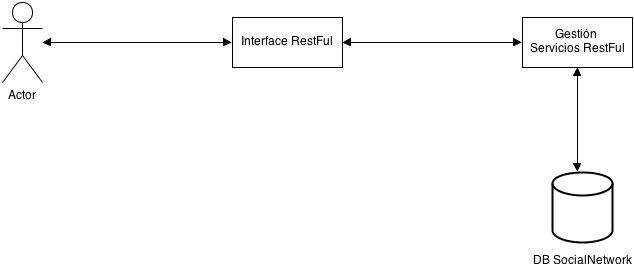
\includegraphics[width=8cm,height=4cm]{Figuras/ArqServRestFul.png}
\end{center}
\caption{\label{ArqServRestFul} Arquitectura de la Interface RestFul}
\end{figure}

\section{Casos de uso para la Interface RestFul}
En éste apartado, vamos a estudiar, mediante el diagrama de casos de uso mostrado en la imagen \ref{imgCasosUsoRestFul}, las posibles acciones a las que se enfrentará y para las que está diseñada la Inteface RestFul y el resto de componentes que necesita para interactuar.
\begin{figure}[h]
\begin{center}
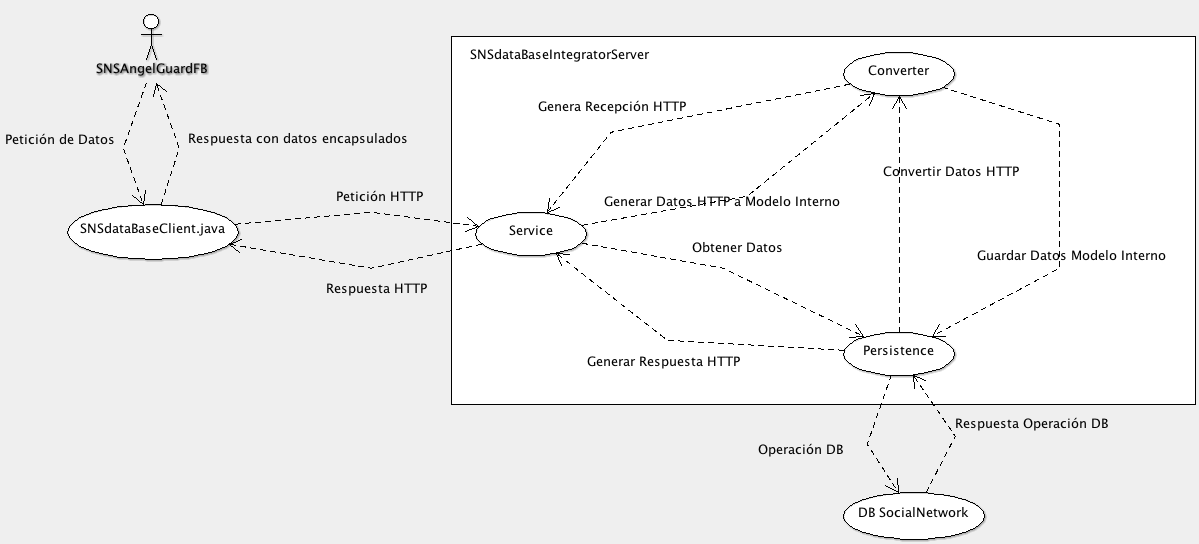
\includegraphics[width=17cm,height=11cm]{Figuras/imgCasosUsoRestFul.png}
\end{center}
\caption{\label{imgCasosUsoRestFul} Diagrama de Casos de Uso de la Interface RestFul}
\end{figure}
\bigskip
\par
El diagrama de casos de uso seguirá la siguiente secuencia:
\begin{enumerate}
\item La aplicación \textbf{SNSAngelGuardFB} generará una operación de datos, bien sea de petición, de actualización o de eliminación. A ésta petición irán encapsulados todos los datos necesarios para realizarla y la URI correspondiente al objeto que se quiere añadir, actualizar o eliminar de la base de datos.
\item La clase \textbf{SNSdataBaseClient.java} generará la operación HTTP necesaria para la operación y la enviará via HTTP al proyecto que se encargará de gestionar los Servicios RestFul junto con las operaciones con la base de datos, en última instancia. La clase SNSdataBaseClient.java contendrá una serie de métodos a los que se invocará para acceder a dichos servicios. Esta será nuestra Interface RestFul en la práctica, ya que será la encargada de los envíos mediante las operaciones HTTP mencionadas anteriormente y de la recepción de las respuestas generadas encapsulando éstas en los tipos de datos necesarios para ser tratadas.
\item Cuando se invoca uno de los métodos de la clase SNSdataBaseClient.java, se envia la petición HTTP al proyecto \textbf{SNSdataBaseIntegratorServer}, quien será el encargado de interactuar con la base de datos. Este proyecto se substenta sobre tres pilares básicos:
\begin{enumerate}
\item El paquete \textbf{service} contendrá, para cada recurso, las clases necesarias que son las que ofrecen los Servicios RestFul que son invocados por la Interface, es decir, cada método que se invoca tiene una entrada en estas clases. Serán las encargadas de recepcionar la petición, analizar mediante la URI recibida a qué objeto se refiere y se debe tratar y, finalmente, enviar la respuesta de la operación.
\item Cuando llega una petición, bien sea de consulta o de actualización, se deberán parsear los datos recibidos de la operación al modelo interno de análisis. Estas operaciones serán realizadas por el paquete \textbf{converter} el cual, para cada recurso de la base de datos, tendrá una serie de estructuras que recibirán los datos de la petición HTTP y los convertirán a datos internos para que puedan ser procesados.
\item Tras realizar el parseo conveniente de los datos, éstos serán enviados a la clase que corresponda, según el recurso, del paquete \textbf{persistence}, el cual, para cada recurso de la base de datos, tendrá una serie de estructuras que serán, en último término, las encargadas de realizar la operación en base de datos y propagar la respuesta que a ésta se produzca, a su nivel superior, es decir, a la clase que corresponda del paquete \textbf{service}, el cual será capaz de propagarlo hasta la Interface RestFul.
\end{enumerate}
\item Una vez que la respuesta ha llegado, el método de la clase SNSdataBaseClient.java parseará el objeto al tipo de datos que se le haya indicado en la petición y propagará la respuesta a su nivel superior, es decir, al método de la aplicación SNSAngelGuardFB que lo haya invocado.
\item Finalmente, al llegar la respuesta al método que originó toda la operación, se analizará el código de respuesta, se obtendrán los datos en caso afirmativo y se continuará con la ejecución de la aplicación.
\end{enumerate}

\section{Projecto SNSdataBaseIntegratorServer}
\textbf{SNSdataBaseIntegratorServer} será el encargado de realizar toda la gestión de los servicios RestFul y, tras evaluar las peticiones, acceder a la base de datos SocialNetwork y realizar la operación que se ha enviado. Tras realizar la operación, generará una respuesta en la que irán encapsulados tanto los datos obtenidos como el código de respuesta HTTP(ver \textbf{Anexo \ref{appHttp}}).
\bigskip
\par
Este proyecto está realizado bajo el lenguaje de programación \textbf{Java} y ha sido desarrollado automáticamente por las herramientas de que dispone el entorno de desarrollo \textbf{NetBeans}, las cuales, a partir de una base de datos, en nuestro caso SocialNetwork, generan todos los Servicios RestFul y todas las estructuras necesarias para realizar la gestión de dicha base de datos. Con ésto conseguimos una gestión de la base de datos totalmente independiente y, además, la base de datos puede no estar en la misma máquina que el servidor que ejecuta la operación pero, por el contrario, siempre se deberá tener ejecutando en un servidor web el proyecto SNSdataBaseIntegratorServer para que puedan llevarse a cabo estas operaciones.
\bigskip
\par
Como bien se ha mencionado anteriormente, este proyecto cuenta con los siguientes paquetes:
\begin{enumerate}
\item Paquete \textbf{es.uah.cc.ie.service}: El cual contendrá todos los servicios RestFul de la base de datos.
\item Paquete \textbf{es.uah.cc.ie.converter}: El cual contendrá todas las estructuras necesarias para realizar la conversión de datos de modelo interno a operación HTTP y viceversa.
\item Paquete \textbf{es.uah.cc.ie.persistence}: El cual contendrá todas las estructuras necesarias para, en última instancia, resolver la operación de base de datos referenciada en el Servicio RestFul. 
\end{enumerate}
\bigskip
\par
La estructura de paquetes puede verse reflejada en la imagen \ref{imgPackageSNSdataBaseIntegratorServer}.
\begin{figure}[h]
\begin{center}
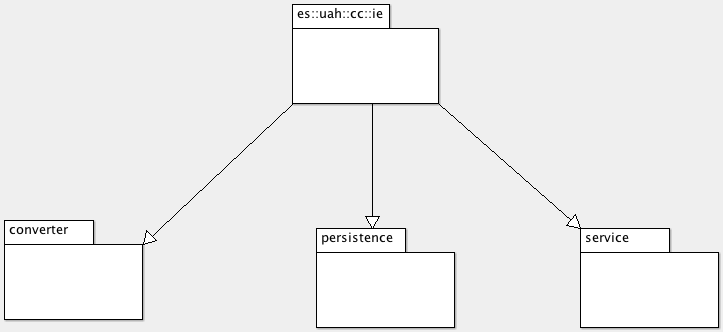
\includegraphics[width=10cm,height=5cm]{Figuras/imgPackageSNSdataBaseIntegratorServer.png}
\end{center}
\caption{\label{imgPackageSNSdataBaseIntegratorServer} Diagrama de paquetes del projecto SNSdataBaseIntegratorServer}
\end{figure}
Para cada recurso, cada paquete contendrá dos estructuras necesarias para su procesamiento( salvo el paquete \textbf{persistence}, que únicamente contendrá una clase por recurso), la estructura que procesa una unidad y la estructura que procesa un conjunto de unidades del mismo recurso. Por ejemplo, si queremos ver las estructuras necesarias para gestionar la tabla user, la imagen \ref{imgPackUser} nos despejará cualquier tipo de duda.
\begin{figure}[h]
\begin{center}
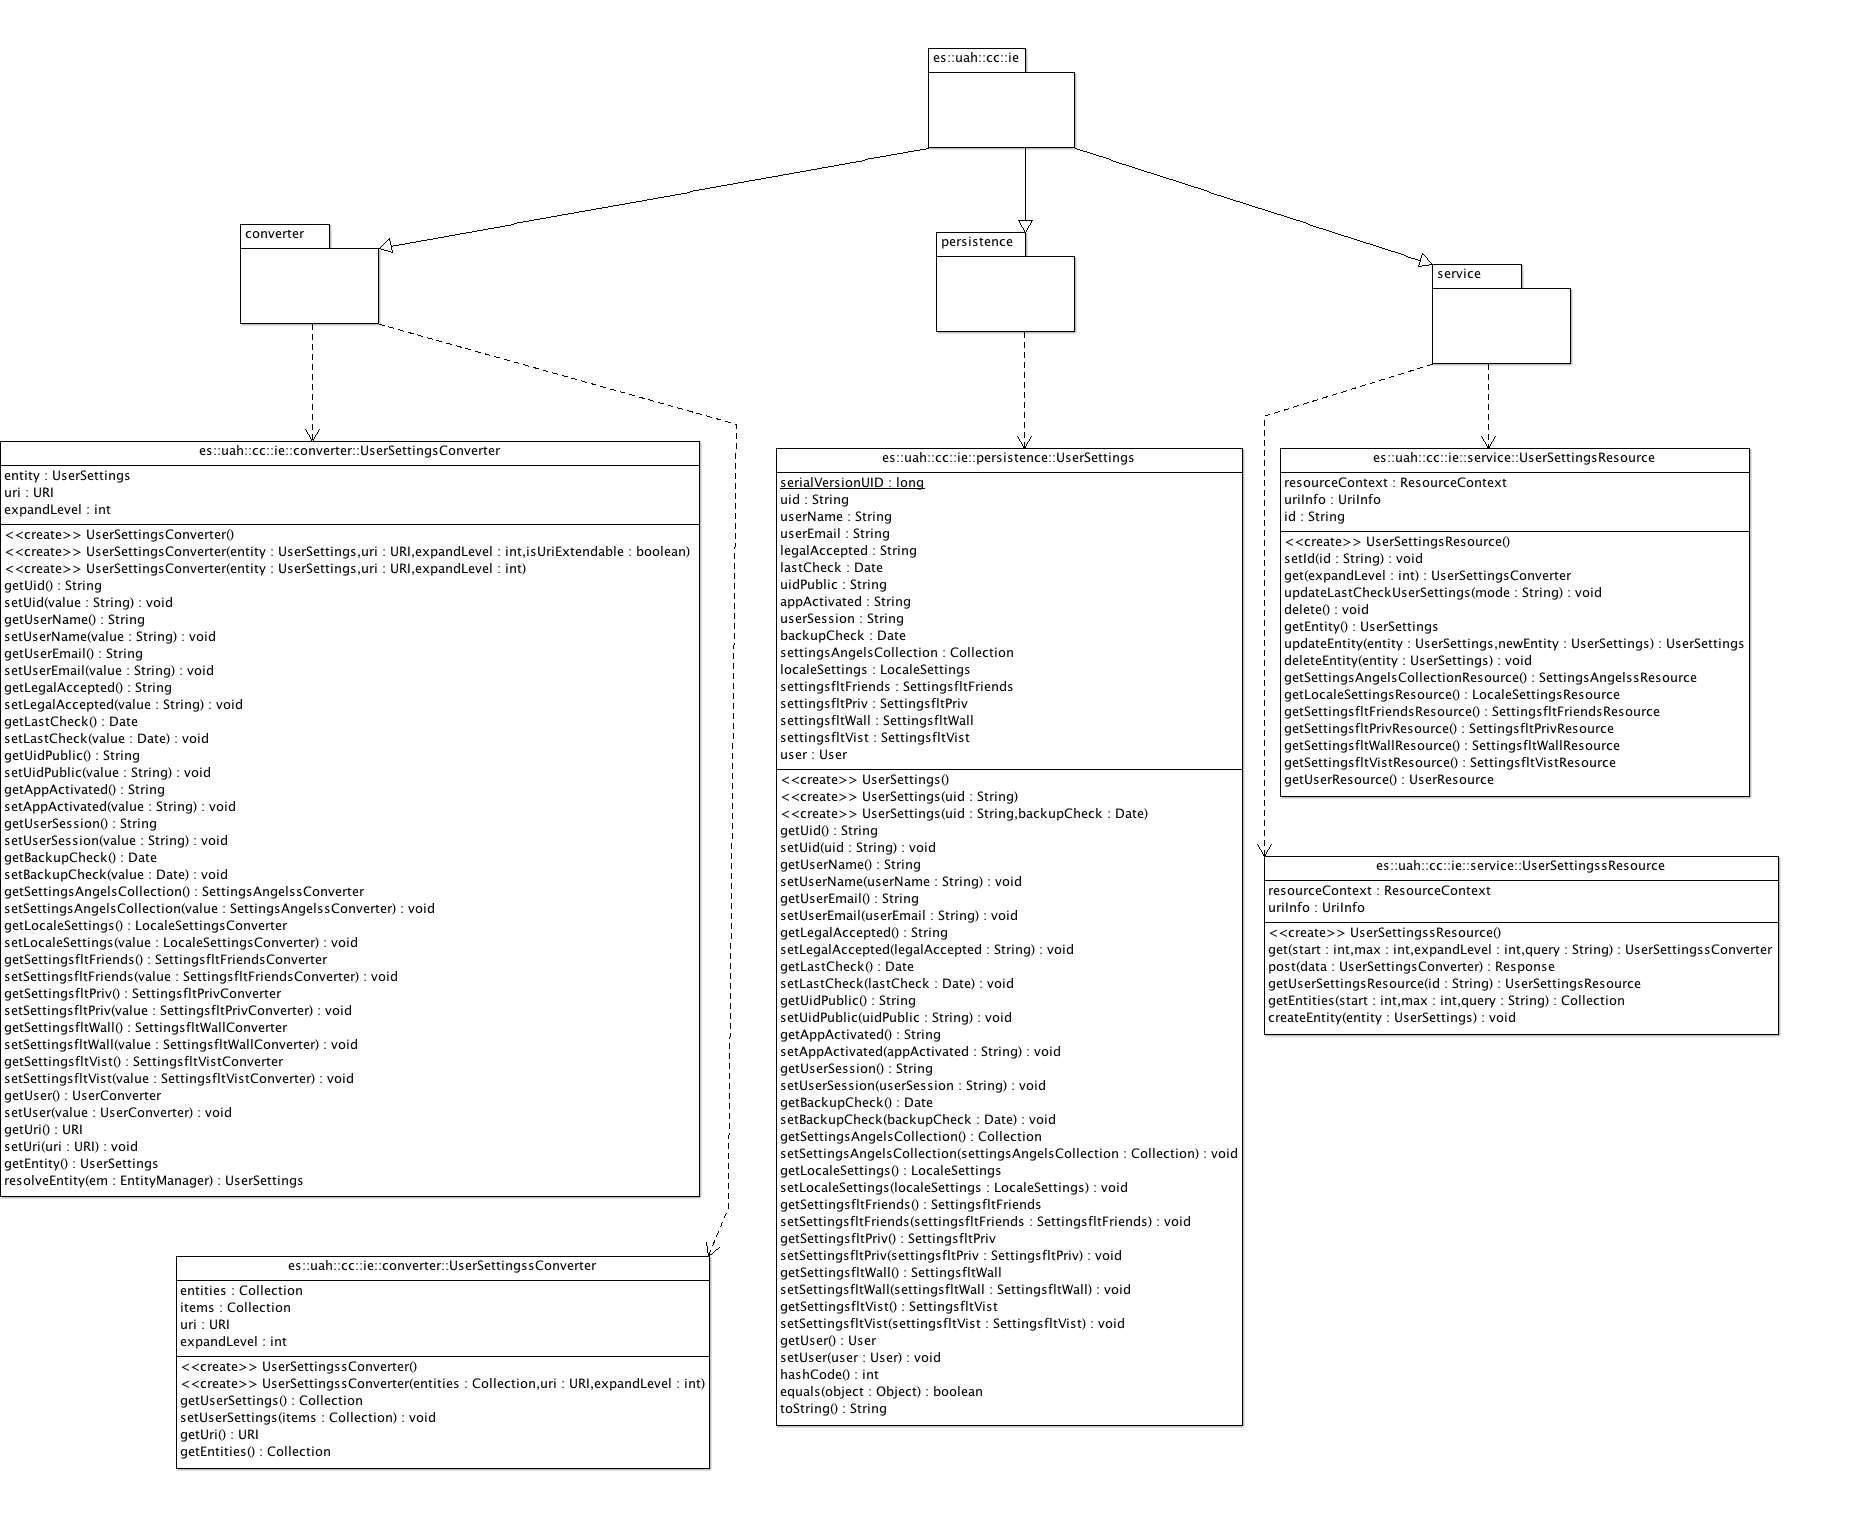
\includegraphics[width=18cm,height=15cm]{Figuras/imgPackUser.png}
\end{center}
\caption{\label{imgPackUser} Diagrama de clases para el recurso UserSettings}
\end{figure}

\subsection{Paquete es.uah.cc.ie.service}
Este paquete contendrá todo el soporte a una petición de un Servicio RestFul. En éste paquete se encontrará dos clases por cada recurso. La clase que gestiona una única entidad tendrá los siguientes componentes:
\begin{enumerate}
\item Atributo \textbf{ResourceContext}: Irá acompañado de la anotación \textbf{@Context}. Servirá para obtener el contexto en el que se está ejecutando el recurso y obtener su referencia física.\begin{verbatim}protected ResourceContext resourceContext;\end{verbatim} 
\item Atributo \textbf{UriInfo}: También irá acompañado de la anotación \textbf{@Context}. En él se almacenará la URI absoluta de acceso al recurso que se está procesando. \begin{verbatim}protected UriInfo uriInfo;\end{verbatim} 
\item Atributo \textbf{String id}: Almacenará el ID del objeto al que hace referencia dentro de la base de datos. \begin{verbatim}protected String id;\end{verbatim} 
\item Método \textbf{get}: Irá precedido de la anotación \textbf{@GET}. Obtendrá un objeto de la base de datos indicado por el parámetro \textbf{ExpandLevel}, que por defecto valdrá 1. Se podrá indicar, mediante la anotación \textbf{@Produces}, en qué formato se van a devolver los datos que ésta llamada produzca, en nuestro caso los datos se enviarán tanto en XML como en JSON, siendo éste último el formato elegido para la recepción.
\item Método \textbf{put}: Irá precedido de la anotación \textbf{@PUT}. Actualizará un determinado objeto de la base de datos. En éste caso, irá acompañado de la anotación \textbf{@Consumes}, que indicará al método qué tipo de datos va a recibir. En nuestro caso, podrá recibir tanto en formato XML como en JSON.
\item Método \textbf{delete}: Irá precedido de la anotación \textbf{@DELETE}. Eliminará un objeto entero, con todas sus relaciones, de la base de datos. No recibirá ningún parámetro, sino que mediante el atributo \textbf{id} sabrá qué entidad es la que procederá a eliminar.
\end{enumerate}
El resto de métodos que se definen en esta clase dependerá únicamente del tipo de recurso que se esté gestionando.
\bigskip
\par
La clase que gestiona un conjunto de entidades se relacionará directamente con la clase anterior para cada una de ellas. Aun así, deberá definir los siguientes componentes:
\begin{enumerate}
\item Atributo \textbf{ResourceContext}: Irá acompañado de la anotación \textbf{@Context}. Servirá para obtener el contexto en el que se está ejecutando el recurso y obtener su referencia física.\begin{verbatim}protected ResourceContext resourceContext;\end{verbatim} 
\item Atributo \textbf{UriInfo}: También irá acompañado de la anotación \textbf{@Context}. En él se almacenará la URI absoluta de acceso al recurso que se está procesando. \begin{verbatim}protected UriInfo uriInfo;\end{verbatim} 
\item Método \textbf{get}: Irá precedido de la anotación \textbf{@GET}. Obtendrá un conjunto de objetos de la base de datos. Se podrá indicar, mediante la anotación \textbf{@Produces}, en qué formato se van a devolver los datos que ésta llamada produzca, en nuestro caso los datos se enviarán tanto en XML como en JSON, siendo éste último el formato elegido para la recepción. En éste caso, el método recibirá los siguientes parámetros siendo totalmente configurables desde la llamada al Servicio RestFul:
\begin{enumerate}
\item \textbf{int start}: Indicará el valor de inicio a la hora de tomar entidades en la consulta. Su valor por defecto será 0.
\item \textbf{int max}: Indicará el número máximo de entidades a devolver en la consulta. Su valor por defecto será 10.
\item \textbf{int expandLevel}: Indicará los niveles hasta los que se puede realizar la consulta. Su valor por defecto será 1.
\item \textbf{String query}: Indicará la sentencia SQL que va a ejecutar.
\end{enumerate}
\item Método \textbf{post}: Irá precedido de la anotación \textbf{@POST}. Actualizará un determinado objeto de la base de datos. En éste caso, irá acompañado de la anotación \textbf{@Consumes}, que indicará al método qué tipo de datos va a recibir. En nuestro caso, podrá recibir tanto en formato XML como en JSON. Recibirá una instancia del objeto que va a actualizar en la base de datos parseado al modelo interno de ésta.
\item Método de acceso a una entidad: Se diferencia del resto porque va precedido de la anotación \textbf{@Path} seguido del UID del objeto en cuestión. Devolverá el objeto de la base de datos referenciado por el parámetro UID de la anotación. 
\end{enumerate}

\subsection{Paquete es.uah.cc.ie.converter}
El paquete \textbf{es.uah.cc.ie.converter} será el encargado de transformar los tipos de datos que reciba de las peticiones HTTP de datos, en formato XML o JSON, y transformarlos al modelo interno de datos del paquete \textbf{es.uah.cc.ie.persistence} para que puedan ser tratados y almacenados en la base de datos SocialNetwork. Realizará el proceso también a la inversa, es decir, recibirá datos de la base de datos SocialNetwork y los transformará en un objeto de formato XML o JSON, dependiendo del valor indicado en la llamada al Servicio RestFul.
\bigskip
\par
Al igual que el paquete \textbf{es.uah.cc.ie.service}, contará con dos clases para cada recurso, una para el tratamiento de la unidad y la otra para el tratamiento de un conjunto de unidades de un recurso determinado.
\bigskip
\par
Los componentes comunes a todas las estructuras que gestionan una única unidad serán los siguientes:
\begin{enumerate}
\item Todas éstas clases, en su definición, irán precedidas de la anotación \textbf{@XmlRootElement}, perteneciente al paquete \textbf{javax.xml.bind.annotation}, seguido del nombre del recurso al que hace referencia. Para el recurso \textbf{userSettings}, su definición será la siguiente:
\begin{verbatim}
@XmlRootElement(name = "userSettings")
public class UserSettingsConverter {
...
... Definición de atributos y métodos de clase
...
}
\end{verbatim} 
\item Atributo \textbf{recurso-entidad} a la que hace referencia: Tendrá como atributo de clase la entidad a la que está asociada la clase del paquete \textbf{es.uah.cc.ie.persistence}. En nuestro caso, para el recurso \textbf{userSettings}, dispondrá del siguiente atributo: \begin{verbatim}private UserSettings entity;\end{verbatim}
\item Atributo \textbf{URI}: Este atributo pertenecerá al paquete de definición \textbf{java.net}. Indicará la URI propia del objeto al que hace referencia. En nuestro caso, para el recurso \textbf{userSettings}, su definición será la siguiente: \begin{verbatim}private URI uri;\end{verbatim}
\item Atributo \textbf{expandLevel}: Este atributo será de tipo \textbf{int} e indicará el nivel al que se debe acceder dentro de la jerarquia del recurso. Su valor por defecto será 1 y su definición, para el recurso \textbf{userSettings}, será la siguiente:\begin{verbatim}private int expandLevel;\end{verbatim}
\item Método \textbf{getEntity}: Este método devolverá un objeto de tipo \textbf{es.uah.cc.ie.persistence} asociado al recurso dependiendo del valor del atributo \textbf{recurso-entidad} del objeto. Su definición irá precedida de la anotación \textbf{@XmlTransient}, la cual pertenecerá al paquete de definición \textbf{javax.xml.bind.annotation}, y servirá para establecer un mapeo recurso-entidad y evitar conflictos con el resto de recursos. Para el recurso \textbf{userSettings}, su definición será la siguiente:
\begin{verbatim}
@XmlTransient
public UserSettings getEntity() {
...
... Definición del método
...
}
\end{verbatim}
\item Método \textbf{resolveEntity}: Este método recibirá un objeto \textbf{EntityManager}, del paquete de definición \textbf{javax.persistence}, de la operación SQL correspondiente, y devolverá un objeto del paquete \textbf{es.uah.cc.ie.persistente} asociado al recurso. Será el encargado de obtener del resultado de una operación de base de datos la entidad y todos los datos a la que ésta hace referencia. Para el recurso \textbf{userSettings}, su definición será la siguiente:
\begin{verbatim}
public UserSettings resolveEntity(EntityManager em) {
...
... Definición del método
...
}
\end{verbatim}
\item Conjunto de métodos para obtener los atributos de la entidad a la que se hace referencia: Estos métodos serán getters y setters asociados al recurso al que hace referencia. Los métodos getters irán precedidos de la anotación \textbf{@XmlElement}, perteneciente al paquete de definición \textbf{javax.xml.bind.annotation}, seguido del nombre del atributo del recurso. Estos métodos leerán directamente del objeto de intercambio XML o JSON el atributo al que hacen referencia y lo establecerán en el modelo interno necesario para el procesamiento de datos en la base de datos.
\end{enumerate}
\bigskip
\par
La definición de componentes para la clase que establece el conjunto de unidades de un recurso será la siguiente:
\begin{enumerate}
\item Este tipo de clases contará en su definición con la anotación \textbf{@XmlRootElement}, perteneciente al paquete \textbf{javax.xml.bind.annotation}, seguido del nombre del recurso al que hace referencia. Notesé que al tratarse de un conjunto de recursos, el recurso para este caso será tratado de manera diferente, por lo que el nombre será distinto. Todos los recursos que hagan referencia a un conjunto de recursos estarán denominados con la nomenclatura \textbf{NombreRecurso + s}, haciendo referencia a la pluralidad del recurso que se está tratando. Para el conjunto \textbf{userSettings}, su definición de clase será la siguiente:
\begin{verbatim}
@XmlRootElement(name = "userSettingss")
public class UserSettingssConverter {
...
... Definición de clase
...
}
\end{verbatim} 
\item Atributo \textbf{Collection<Recurso>}: Indicará la colección de recursos a la que hace referencia. Los recursos pertenecerán al paquete \textbf{es.uah.cc.ie.persistence}. Para el caso del recurso \textbf{userSettingss}, su definición será la siguiente: \begin{verbatim}private Collection<UserSettings> entities;\end{verbatim}
\item Atributo \textbf{Collection<RecursoConverter>}: Indicará la colección de recursos del paquete \textbf{es.uah.cc.ie.converter} que han sido parseados directamente del objeto de intercambio XML o JSON y están preparados para ser persistidos. En el caso del recurso \textbf{userSettingss}, su definición será la siguiente: \begin{verbatim}private Collection<UserSettingsConverter> items;\end{verbatim}.
\item Atributo \textbf{URI}: Este atributo pertenecerá al paquete de definición \textbf{java.net}. Indicará la URI propia del objeto al que hace referencia. En nuestro caso, para el recurso \textbf{userSettingss}, su definición será la siguiente: \begin{verbatim}private URI uri;\end{verbatim}
\item Atributo \textbf{expandLevel}: Este atributo será de tipo \textbf{int} e indicará el nivel al que se debe acceder dentro de la jerarquia del recurso. Su valor por defecto será 1 y su definición, para el recurso \textbf{userSettingss}, será la siguiente:\begin{verbatim}private int expandLevel;\end{verbatim}
\item Método \textbf{getEntities}: Devolverá un objeto de tipo \textbf{Collection<Recurso>} asociado al recurso, del paquete \textbf{es.uah.cc.ie.persistence}, dependiendo del valor del atributo \textbf{recurso-entidad} del objeto. Su definición irá precedida de la anotación \textbf{@XmlTransient}, la cual pertenecerá al paquete \textbf{javax.xml.bind.annotation}, y servirá para establecer un mapeo recurso-entidad y evitar conflictos con el resto de recursos. Para el recurso \textbf{userSettingss}, su definición será la siguiente:
\begin{verbatim}
@XmlTransient
public Collection<UserSettings> getEntities() {
...
... Definición del método
...
}
\end{verbatim}
\end{enumerate}

\subsection{Paquete es.uah.cc.ie.persistence}
El paquete \textbf{es.uah.cc.ie.persistence} contendrá todas las estructuras necesarias para, en última instancia, persistir el objeto del recurso referenciado en base de datos. Por cada recurso existirá una única clase que contendrá todos los atributos de la tabla de la base de datos SocialNetwork a la que hace referencia junto con todas las definiciones de sus dependencias con otras tablas. Se tomará como ejemplo el recurso \textbf{userSettings}, que hará referencia a la tabla de base de datos \textbf{user\_settings} con la que trabajará exclusivamente. Sus componentes serán los siguientes(que se podrán hacer extensibles al resto de recursos):
\begin{enumerate}
\item Definición de la clase: Su definición será un conjunto de parámetros que se explicarán a continuación:
\begin{enumerate}
\item Anotación \textbf{@Entity}: Pertenecerá al paquete de definición \textbf{javax.persistence}. Con esta anotación se indica que estamos tratando de una Entidad mapeada directamente en base de datos.
\item Anotación \textbf{@Table}: Pertenecerá al paquete de definición \textbf{javax.persistence}. Esta anotación irá seguida del nombre de la tabla con la que está mapeada.
\item Anotación \textbf{@NamedQueries}: Pertenecerá al paquete de definición de java \textbf{javax.persistence}. Ésta contendrá todas las definiciones de las posibles querys que pueden ser invocadas para cada uno de los atributos de la tabla. Para cada una de las definiciones, se utilizará la anotación \textbf{@NamedQuery}, que pertenecerá al mismo paquete de definición.
\item Implementará a la interface \textbf{Serializable}, perteneciente al paquete de definición \textbf{java.io}. Servirá para poder serializar un objeto y poder enviarlo a través del protocolo HTTP.
\end{enumerate}
Con todas estas indicaciones, la definición de la entidad \textbf{userSettings} será de la siguiente forma:
\begin{verbatim}
@Entity
@Table(name = "user_settings")
@NamedQueries({
    @NamedQuery(name = "UserSettings.findAll", query = "SELECT u FROM 
         UserSettings u"),
    @NamedQuery(name = "UserSettings.findByUid", query = "SELECT u FROM 
 	       UserSettings u WHERE u.uid = :uid"),
    @NamedQuery(name = "UserSettings.findByUserName", query = "SELECT u 
         FROM UserSettings u WHERE u.userName = :userName"),
    @NamedQuery(name = "UserSettings.findByUserEmail", query = "SELECT u 
         FROM UserSettings u WHERE u.userEmail = :userEmail"),
    @NamedQuery(name = "UserSettings.findByLegalAccepted", query = "SELECT u
         FROM UserSettings u WHERE u.legalAccepted = :legalAccepted"),
    @NamedQuery(name = "UserSettings.findByLastCheck", query = "SELECT u 
         FROM UserSettings u WHERE u.lastCheck = :lastCheck"),
    @NamedQuery(name = "UserSettings.findByUidPublic", query = "SELECT u 
         FROM UserSettings u WHERE u.uidPublic = :uidPublic"),
    @NamedQuery(name = "UserSettings.findByAppActivated", query = "SELECT u 
         FROM UserSettings u WHERE u.appActivated = :appActivated"),
    @NamedQuery(name = "UserSettings.findByUserSession", query = "SELECT u 
         FROM UserSettings u WHERE u.userSession = :userSession"),
    @NamedQuery(name = "UserSettings.findByBackupCheck", query = "SELECT u 
         FROM UserSettings u WHERE u.backupCheck = :backupCheck")})
public class UserSettings implements Serializable {
...
... Definición de la Entidad
...
}
\end{verbatim}
\item Conjunto de métodos de acceso a cada uno de los atributos de la tabla: Para acceder al valor de cada uno de los atributos, en cada clase existirán metodos estructurales(get y set) para cada uno de los atributos.
\end{enumerate}

\section{Interface RestFul SNSdataBaseClient.java}
Hasta este punto, hemos realizado el estudio, el análisis y el diseño de todos los servicios RestFul que van a poner en funcionamiento nuestra base de datos de una forma independiente y totalmente transparente al desarrollador. Mediante un servidor web pondremos en funcionamiento el proyecto SNSdataBaseIntegratorServer y tendremos a disposición todo el potencial de nuestra base de datos.
\bigskip
\par
Ahora bien, el tema que nos ocupa, es el estudio de cómo poder llamar a los servicios RestFul definidos con anterioridad desde nuestra aplicación sin tener que hacer ninguna operación de base de datos en ella. Esto lo conseguimos con la implementación de un fichero cliente que encapsulará, en métodos de llamada, todos los servicios RestFul que sean necesarios para el funcionamiento de nuestra aplicación. Mediante estos sencillos métodos se conseguirá enviar órdenes de base de datos hasta el proyecto SNSdataBaseIntegratorServer por medio del protocolo HTTP y nuestra aplicación será capaz tanto de realizar las llamadas como analizar las respuestas. 
\bigskip
\par
El cliente desarrollado en el fichero \textbf{SNSdataBaseClient.java} es una solución funcional encapsulada en el proyecto \textbf{SNSAngelGuardFB}, que contendrá toda la funcionalidad de la aplicación. Las ventajas de esta implementación radican en el simple hecho de que esta interface podría ser pública, por lo cual, cualquier desarrollador podría tomarla en su proyecto y utilizar todos sus métodos para la gestión de la base de datos SocialNetwork.
\bigskip
\par
En las sucesivas secciones a ésta, se pasará a explicar la estructura de éste fichero y de cada uno de los métodos que han sido desarrollados para conseguir esta solución.

\subsection{Atributos de la clase SNSdataBaseClient.java}
En ésta sección se estudiarán y analizarán los diferentes atributos que contiene la clase \textbf{SNSdataBaseClient.java}, que serán los siguientes:
\begin{enumerate}
\item Atributo \textbf{WebResource}: Mediante este atributo se conseguirán construir recursos web que sean capaces de enviar y procesar respuestas HTTP. Pertenecerá al paquete \textbf{com.sun.jersey.api.client.Client}.
\item Atributo \textbf{Client}: Este atributo permite configurar las propiedades de conexión de un recurso web y crear una conexión, por lo que el atributo \textbf{WebResource} lo utilizará como conexión configurada para enviar peticiones HTTP. Pertenecerá, al igual que el atributo \textbf{WebResource}, al paquete \textbf{com.sun.jersey.api.client.Client}.
\item Constante \textbf{BASE\_URI}: Será una constante de tipo \textbf{String} y contendrá la dirección en la que está instalado el proyecto que gestiona los servicios RestFul de la base de datos que, en nuestro caso, será el proyecto \textbf{SNSdataBaseIntegratorServer}. Para un entorno local de pruebas, el valor de éste atributo será el siguiente: \begin{verbatim}"http://localhost:8080/SNSdataBaseIntegratorServer/resources/"\end{verbatim}
\end{enumerate}

\subsection{Métodos de la clase SNSdataBaseClient.java}
En ésta sección se analizarán todos los métodos que van a acceder a Servicios RestFul de nuestra base de datos y, como tal, conformarán una API pública que podrá ser accesible en un futuro por cualquier desarrollador. Como nomenclatura estándar para su definición, se utilizará el formato \textbf{NombreTablaDB\_NombreMetodo}. En las secciones siguientes se irán explicando cada uno de ellos con el nivel de detalle necesario.

\subsubsection{Método userSettings\_getEntities}
Este método obtiene todas los registros de la tabla \textbf{user\_settings}. Será de utilidad en los procesos offline de la aplicación. Su información será la siguiente:
\begin{enumerate}
\item Entrada: Recibirá un parámetro con el tipo de dato que queremos a la salida \textbf{Class<T> responseType}.
\item Salida: Devolverá el tipo de dato que se ha indicado en el parámetro de entrada \textbf{responseType}.
\item Podrá devolver el tipo de excepción \textbf{UniformInterfaceException}.
\end{enumerate}
\bigskip
\par
Su definición será la siguiente:
\begin{verbatim}public <T> T userSettings_getEntities(Class<T> responseType) 
                                     throws UniformInterfaceException \end{verbatim}

\subsubsection{Método userSettings\_getUserByUidPublic}
Este método obtiene el usuario de la tabla \textbf{user\_settings} que coincida con el parámetro \textbf{uidPublic}, el cual será su \textbf{identificador publico}, es decir, el identificador que puede observarse públicamente, obtenido de cifrar el identificador del usuario en Facebook con una cláve privada proporcionada por el desarrollador de la aplicación. Será de utilidad cuando un ángel quiera acceder a la información del usuario que le ha enviado la petición de seguimiento. Su información será la siguiente:
\begin{enumerate}
\item Entrada: Recibirá los siguientes parámentros:
\begin{enumerate}
\item \textbf{Class<T> responseType}: Contendrá el tipo de dato que queremos a la salida. 
\item \textbf{String uidPublic}: Contendrá el identificador público del usuario que ejecuta la aplicación.
\end{enumerate}
\item Salida: Devolverá toda la información del usuario al que referencia su uid pública en el tipo de dato que se ha indicado en el parámetro de entrada \textbf{responseType}.
\item Podrá devolver el tipo de excepción \textbf{UniformInterfaceException}.
\end{enumerate}
\bigskip
\par
Su definición será la siguiente:
\begin{verbatim}public <T> T userSettings_getUserByUidPublic(Class<T> responseType, 
                                     String uidPublic) 
                                     throws UniformInterfaceException \end{verbatim}

\subsubsection{Método userSettings\_setUpdateTime}
Este método actualiza la fecha \textbf{lastCheck} o \textbf{backUpCheck} a la fecha en la que se está realizando la operación y, además, actualiza la sesión del usuario a la última sesión de conexión de Facebook. Que se actualice una u otra fecha dependerá del valor del parámetro \textbf{mode}. Su información será la siguiente:
\begin{enumerate}
\item Entrada: Recibirá los siguientes parámentros:
\begin{enumerate}
\item \textbf{Class<T> responseType}: Contendrá el tipo de dato que queremos a la salida. 
\item \textbf{String uid}: Contendrá el uid del usuario que ejecuta la aplicación.
\item \textbf{String mode}: Si mode es ``1'', se actualizará la fecha \textbf{lastCheck}. Si por el contrario es``0'', se actualizará la fecha \textbf{backUpCheck}.
\item \textbf{String oauhToken}: Contendrá la nueva sesión para el usuario creada desde Facebook.
\end{enumerate}
\item Salida: Devolverá la información del usuario con la fecha \textbf{lastCheck} o \textbf{backUpCheck} actualizada.
\end{enumerate}
\bigskip
\par
Su definición será la siguiente:
\begin{verbatim}public <T> T userSettings_setUpdateTime(Class<T> responseType, 
                                        String uid, 
                                        String mode) \end{verbatim}

\subsubsection{Método userSettings\_setNewEntityUserSettings}
Este método introduce un nuevo usuario, con toda su información, en la tabla \textbf{user\_settings}. Su información será la siguiente:
\begin{enumerate}
\item Entrada: Recibirá los siguientes parámentros:
\begin{enumerate}
\item \textbf{Class<T> responseType}: Contendrá el tipo de dato que queremos a la salida. 
\item \textbf{Object requestEntity}: Objeto, en formato XML o JSON, que contendrá todos los datos del usuario que se da de alta en la tabla.
\end{enumerate}
\item Salida: Devolverá la información del usuario que se ha introducido.
\item Podrá devolver el tipo de excepción \textbf{UniformInterfaceException}.
\end{enumerate}
\bigskip
\par
Su definición será la siguiente:
\begin{verbatim}public <T> T userSettings_setNewEntityUserSettings(Class<T> responseType, 
                                                Object requestEntity) 
                                                throws UniformInterfaceException \end{verbatim}

\subsubsection{Método userSettings\_getUserSettingsByUid}
Este método devuelve toda la información del usuario de la tabla \textbf{user\_settings} al que pertenece el parámetro de entrada \textbf{uid}. Su información será la siguiente:
\begin{enumerate}
\item Entrada: Recibirá los siguientes parámentros:
\begin{enumerate}
\item \textbf{Class<T> responseType}: Contendrá el tipo de dato que queremos a la salida. 
\item \textbf{String uid}: Identificador del usuario que queremos obtener.
\end{enumerate}
\item Salida: Devolverá la información del usuario al que pertenezca el parámetro \textbf{uid} o, si no existe, devolverá una excepción \textbf{UniformInterfaceException} con el código de error HTTP asociado.
\end{enumerate}
\bigskip
\par
Su definición será la siguiente:
\begin{verbatim}public <T> T userSettings_getUserSettingsByUid(Class<T> responseType, 
                          		            String uid) 
                           		   throws UniformInterfaceException \end{verbatim}

\subsubsection{Método userSettings\_setNewAngelsCollectionByUid}
Este método establece un nuevo ángel en la colección de un usuario de la tabla \textbf{user\_settings}, al que pertenece el parámetro de entrada \textbf{uidAngel}. Para que se lleve a cabo, dentro del objeto de entrada \textbf{Object requestEntity} deberá figurar la URI que relacione al Ángel con el usuario. Su información será la siguiente:
\begin{enumerate}
\item Entrada: Recibirá los siguientes parámentros:
\begin{enumerate}
\item \textbf{Class<T> responseType}: Contendrá el tipo de dato que queremos a la salida. 
\item \textbf{String uidAngel}: Identificador del nuevo Ángel.
\item \textbf{Object requestEntity}: Información del nuevo Ángel.
\end{enumerate}
\item Salida: Devolverá la información del nuevo Ángel o una excepción \textbf{UniformInterfaceException} con el código de error HTTP asociado.
\end{enumerate}
\bigskip
\par
Su definición será la siguiente:
\begin{verbatim}public <T> T userSettings_setNewAngelsCollectionByUid(Class<T> responseType, 
					String uidAngel, 
					Object requestEntity) 
					throws UniformInterfaceException \end{verbatim}

\subsubsection{Método localeSettings\_getLocaleSettingsByUid}
Obtiene los recursos de idioma según el parámetro de entrada \textbf{uid}. Su información será la siguiente:
\begin{enumerate}
\item Entrada: Recibirá los siguientes parámentros:
\begin{enumerate}
\item \textbf{Class<T> responseType}: Contendrá el tipo de dato que queremos a la salida. 
\item \textbf{String uid}: Identificador de los recursos de idioma según la tabla \textbf{locale\_settings}.
\end{enumerate}
\item Salida: Devolverá los recursos de idioma asociados al parámetro \textbf{uid} o una excepción \textbf{UniformInterfaceException} con el código de error HTTP asociado.
\end{enumerate}
\bigskip
\par
Su definición será la siguiente:
\begin{verbatim}public <T> T localeSettings_getLocaleSettingsByUid(Class<T> responseType,
					String uid) 
					throws UniformInterfaceException\end{verbatim}

\subsubsection{Método settingsFltWall\_getUserByUid}
Obtiene la configuración del filtro de control de lenguaje para el usuario de la tabla \textbf{user\_settings} al que corresponde el identificador de entrada \textbf{uid}. Su información será la siguiente:
\begin{enumerate}
\item Entrada: Recibirá los siguientes parámentros:
\begin{enumerate}
\item \textbf{Class<T> responseType}: Contendrá el tipo de dato que queremos a la salida. 
\item \textbf{String uid}: Identificador del usuario de la tabla \textbf{user\_settings}.
\end{enumerate}
\item Salida: Devolverá la configuración del filtro de control de lenguaje asociada al parámetro \textbf{uid} o una excepción \textbf{UniformInterfaceException} con el código de error HTTP asociado.
\end{enumerate}
\bigskip
\par
Su definición será la siguiente:
\begin{verbatim}public <T> T settingsFltWall_getUserByUid(Class<T> responseType, 
					String uid) 
					throws UniformInterfaceException\end{verbatim}

\subsubsection{Método settingsFltWall\_setNewUser}
Establece la configuración inicial del filtro de control de lenguaje para el usuario de la tabla \textbf{user\_settings}. Su información será la siguiente:
\begin{enumerate}
\item Entrada: Recibirá los siguientes parámentros:
\begin{enumerate}
\item \textbf{Class<T> responseType}: Contendrá el tipo de dato que queremos a la salida. 
\item \textbf{Object requestEntity}: Configuración inicial del filtro de control de lenguaje.
\end{enumerate}
\item Salida: Devolverá la configuración inicial del filtro de control de lenguaje o una excepción \textbf{UniformInterfaceException} con el código de error HTTP asociado.
\end{enumerate}
\bigskip
\par
Su definición será la siguiente:
\begin{verbatim}public <T> T settingsFltWall_setNewUser(Class<T> responseType, 
					Object requestEntity) 
					throws UniformInterfaceException\end{verbatim}


\subsubsection{Método settingsFltWall\_setFilterByUid}
Establece la configuración del filtro de control de lenguaje para el usuario de la tabla \textbf{user\_settings} que identifica el parámetro de entrada \textbf{uid}. Su información será la siguiente:
\begin{enumerate}
\item Entrada: Recibirá los siguientes parámentros:
\begin{enumerate}
\item \textbf{Class<T> responseType}: Contendrá el tipo de dato que queremos a la salida. 
\item \textbf{String uid}: Identificador del usuario de la tabla \textbf{user\_settings}.
\item \textbf{Object requestEntity}: Nueva configuración del filtro de control de lenguaje.
\end{enumerate}
\item Salida: Devolverá la nueva configuración del filtro de control de lenguaje o una excepción \textbf{UniformInterfaceException} con el código de error HTTP asociado.
\end{enumerate}
\bigskip
\par
Su definición será la siguiente:
\begin{verbatim}public <T> T settingsFltWall_setFilterByUid(Class<T> responseType, 
					String uid, 
					Object requestEntity) 
					throws UniformInterfaceException\end{verbatim}

\subsubsection{Método settingsFltWall\_setLastCheckByUid}
Actualiza el parámetro \textbf{lastCheck} a la hora en que se ejecuta el filtro del usuario que identifica el parámetro de entrada \textbf{uid}. Su información será la siguiente:
\begin{enumerate}
\item Entrada: Recibirá los siguientes parámentros:
\begin{enumerate}
\item \textbf{Class<T> responseType}: Contendrá el tipo de dato que queremos a la salida. 
\item \textbf{String uid}: Identificador del usuario de la tabla \textbf{user\_settings}.
\end{enumerate}
\item Salida: Devolverá la configuración del filtro de control de lenguaje con el nuevo parámetro \textbf{lastCheck} actualizado o una excepción \textbf{UniformInterfaceException} con el código de error HTTP asociado.
\end{enumerate}
\bigskip
\par
Su definición será la siguiente:
\begin{verbatim}public <T> T settingsFltWall_setLastCheckByUid(Class<T> responseType, 
					String uid) 
					throws UniformInterfaceException\end{verbatim}

\subsubsection{Método settingsFltWall\_getAngelsCollectionByUid}
Obtiene la colección de ángeles definidos en el filtro de control de lenguaje del usuario que identifica el parámetro de entrada \textbf{uid}. Su información será la siguiente:
\begin{enumerate}
\item Entrada: Recibirá los siguientes parámentros:
\begin{enumerate}
\item \textbf{Class<T> responseType}: Contendrá el tipo de dato que queremos a la salida. 
\item \textbf{String uid}: Identificador del usuario de la tabla \textbf{user\_settings}.
\end{enumerate}
\item Salida: Devolverá la colección de ángeles definidos para el usuario \textbf{uid} del filtro de control de lenguaje o una excepción \textbf{UniformInterfaceException} con el código de error HTTP asociado.
\end{enumerate}
\bigskip
\par
Su definición será la siguiente:
\begin{verbatim}public <T> T settingsFltWall_getAngelsCollectionByUid(Class<T> responseType, 
					String uid) 
					throws UniformInterfaceException \end{verbatim}



\subsubsection{Método settingsFltFriends\_getUserByUid}
Obtiene la configuración del filtro de control de amigos para el usuario de la tabla \textbf{user\_settings} al que corresponde el identificador de entrada \textbf{uid}. Su información será la siguiente:
\begin{enumerate}
\item Entrada: Recibirá los siguientes parámentros:
\begin{enumerate}
\item \textbf{Class<T> responseType}: Contendrá el tipo de dato que queremos a la salida. 
\item \textbf{String uid}: Identificador del usuario de la tabla \textbf{user\_settings}.
\end{enumerate}
\item Salida: Devolverá la configuración del filtro de control de amigos asociada al parámetro \textbf{uid} o una excepción \textbf{UniformInterfaceException} con el código de error HTTP asociado.
\end{enumerate}
\bigskip
\par
Su definición será la siguiente:
\begin{verbatim}public <T> T settingsFltFriends_getUserByUid(Class<T> responseType, 
					String uid) 
					throws UniformInterfaceException\end{verbatim}

\subsubsection{Método settingsFltFriends\_setNewUser}
Establece la configuración inicial del filtro de control de amigos para el usuario de la tabla \textbf{user\_settings}. Su información será la siguiente:
\begin{enumerate}
\item Entrada: Recibirá los siguientes parámentros:
\begin{enumerate}
\item \textbf{Class<T> responseType}: Contendrá el tipo de dato que queremos a la salida. 
\item \textbf{Object requestEntity}: Configuración inicial del filtro de control de amigos.
\end{enumerate}
\item Salida: Devolverá la configuración inicial del filtro de control de amigos o una excepción \textbf{UniformInterfaceException} con el código de error HTTP asociado.
\end{enumerate}
\bigskip
\par
Su definición será la siguiente:
\begin{verbatim}public <T> T settingsFltFriends_setNewUser(Class<T> responseType, 
					Object requestEntity) 
					throws UniformInterfaceException\end{verbatim}


\subsubsection{Método settingsFltFriends\_setFilterByUid}
Establece la configuración del filtro de control de amigos para el usuario de la tabla \textbf{user\_settings} que identifica el parámetro de entrada \textbf{uid}. Su información será la siguiente:
\begin{enumerate}
\item Entrada: Recibirá los siguientes parámentros:
\begin{enumerate}
\item \textbf{Class<T> responseType}: Contendrá el tipo de dato que queremos a la salida. 
\item \textbf{String uid}: Identificador del usuario de la tabla \textbf{user\_settings}.
\item \textbf{Object requestEntity}: Nueva configuración del filtro de control de amigos.
\end{enumerate}
\item Salida: Devolverá la nueva configuración del filtro de control de amigos o una excepción \textbf{UniformInterfaceException} con el código de error HTTP asociado.
\end{enumerate}
\bigskip
\par
Su definición será la siguiente:
\begin{verbatim}public <T> T settingsFltFriends_setFilterByUid(Class<T> responseType, 
					String uid, 
					Object requestEntity) 
					throws UniformInterfaceException\end{verbatim}

\subsubsection{Método settingsFltFriends\_setLastCheckByUid}
Actualiza el parámetro \textbf{lastCheck} a la hora en que se ejecuta el filtro de control de amigos del usuario que identifica el parámetro de entrada \textbf{uid}. Su información será la siguiente:
\begin{enumerate}
\item Entrada: Recibirá los siguientes parámentros:
\begin{enumerate}
\item \textbf{Class<T> responseType}: Contendrá el tipo de dato que queremos a la salida. 
\item \textbf{String uid}: Identificador del usuario de la tabla \textbf{user\_settings}.
\end{enumerate}
\item Salida: Devolverá la configuración del filtro de control de amigos con el nuevo parámetro \textbf{lastCheck} actualizado o una excepción \textbf{UniformInterfaceException} con el código de error HTTP asociado.
\end{enumerate}
\bigskip
\par
Su definición será la siguiente:
\begin{verbatim}public <T> T settingsFltFriends_setLastCheckByUid(Class<T> responseType, 
					String uid) 
					throws UniformInterfaceException\end{verbatim}

\subsubsection{Método settingsFltFriends\_getAngelsCollectionByUid}
Obtiene la colección de ángeles definidos en el filtro de control de amigos del usuario que identifica el parámetro de entrada \textbf{uid}. Su información será la siguiente:
\begin{enumerate}
\item Entrada: Recibirá los siguientes parámentros:
\begin{enumerate}
\item \textbf{Class<T> responseType}: Contendrá el tipo de dato que queremos a la salida. 
\item \textbf{String uid}: Identificador del usuario de la tabla \textbf{user\_settings}.
\end{enumerate}
\item Salida: Devolverá la colección de ángeles definidos para el usuario \textbf{uid} del filtro de control de amigos o una excepción \textbf{UniformInterfaceException} con el código de error HTTP asociado.
\end{enumerate}
\bigskip
\par
Su definición será la siguiente:
\begin{verbatim}public <T> T settingsFltFriends_getAngelsCollectionByUid(Class<T> responseType, 
					String uid) 
					throws UniformInterfaceException \end{verbatim}





\subsubsection{Método settingsFltPriv\_getUserByUid}
Obtiene la configuración del filtro de control de privacidad para el usuario de la tabla \textbf{user\_settings} al que corresponde el identificador de entrada \textbf{uid}. Su información será la siguiente:
\begin{enumerate}
\item Entrada: Recibirá los siguientes parámentros:
\begin{enumerate}
\item \textbf{Class<T> responseType}: Contendrá el tipo de dato que queremos a la salida. 
\item \textbf{String uid}: Identificador del usuario de la tabla \textbf{user\_settings}.
\end{enumerate}
\item Salida: Devolverá la configuración del filtro de control de privacidad asociada al parámetro \textbf{uid} o una excepción \textbf{UniformInterfaceException} con el código de error HTTP asociado.
\end{enumerate}
\bigskip
\par
Su definición será la siguiente:
\begin{verbatim}public <T> T settingsFltPriv_getUserByUid(Class<T> responseType, 
					String uid) 
					throws UniformInterfaceException\end{verbatim}

\subsubsection{Método settingsFltPriv\_setNewUser}
Establece la configuración inicial del filtro de control de privacidad para el usuario de la tabla \textbf{user\_settings}. Su información será la siguiente:
\begin{enumerate}
\item Entrada: Recibirá los siguientes parámentros:
\begin{enumerate}
\item \textbf{Class<T> responseType}: Contendrá el tipo de dato que queremos a la salida. 
\item \textbf{Object requestEntity}: Configuración inicial del filtro de control de privacidad.
\end{enumerate}
\item Salida: Devolverá la configuración inicial del filtro de control de privacidad o una excepción \textbf{UniformInterfaceException} con el código de error HTTP asociado.
\end{enumerate}
\bigskip
\par
Su definición será la siguiente:
\begin{verbatim}public <T> T settingsFltPriv_setNewUser(Class<T> responseType, 
					Object requestEntity) 
					throws UniformInterfaceException\end{verbatim}


\subsubsection{Método settingsFltPriv\_setFilterByUid}
Establece la configuración del filtro de control de privacidad para el usuario de la tabla \textbf{user\_settings} que identifica el parámetro de entrada \textbf{uid}. Su información será la siguiente:
\begin{enumerate}
\item Entrada: Recibirá los siguientes parámentros:
\begin{enumerate}
\item \textbf{Class<T> responseType}: Contendrá el tipo de dato que queremos a la salida. 
\item \textbf{String uid}: Identificador del usuario de la tabla \textbf{user\_settings}.
\item \textbf{Object requestEntity}: Nueva configuración del filtro de control de privacidad.
\end{enumerate}
\item Salida: Devolverá la nueva configuración del filtro de control de privacidad o una excepción \textbf{UniformInterfaceException} con el código de error HTTP asociado.
\end{enumerate}
\bigskip
\par
Su definición será la siguiente:
\begin{verbatim}public <T> T settingsFltPriv_setFilterByUid(Class<T> responseType, 
					String uid, 
					Object requestEntity) 
					throws UniformInterfaceException\end{verbatim}

\subsubsection{Método settingsFltPriv\_setLastCheckByUid}
Actualiza el parámetro \textbf{lastCheck} a la hora en que se ejecuta el filtro de control de privacidad del usuario que identifica el parámetro de entrada \textbf{uid}. Su información será la siguiente:
\begin{enumerate}
\item Entrada: Recibirá los siguientes parámentros:
\begin{enumerate}
\item \textbf{Class<T> responseType}: Contendrá el tipo de dato que queremos a la salida. 
\item \textbf{String uid}: Identificador del usuario de la tabla \textbf{user\_settings}.
\end{enumerate}
\item Salida: Devolverá la configuración del filtro de control de privacidad con el nuevo parámetro \textbf{lastCheck} actualizado o una excepción \textbf{UniformInterfaceException} con el código de error HTTP asociado.
\end{enumerate}
\bigskip
\par
Su definición será la siguiente:
\begin{verbatim}public <T> T settingsFltPriv_setLastCheckByUid(Class<T> responseType, 
					String uid) 
					throws UniformInterfaceException\end{verbatim}

\subsubsection{Método settingsFltPriv\_getAngelsCollectionByUid}
Obtiene la colección de ángeles definidos en el filtro de control de privacidad del usuario que identifica el parámetro de entrada \textbf{uid}. Su información será la siguiente:
\begin{enumerate}
\item Entrada: Recibirá los siguientes parámentros:
\begin{enumerate}
\item \textbf{Class<T> responseType}: Contendrá el tipo de dato que queremos a la salida. 
\item \textbf{String uid}: Identificador del usuario de la tabla \textbf{user\_settings}.
\end{enumerate}
\item Salida: Devolverá la colección de ángeles definidos para el usuario \textbf{uid} del filtro de control de privacidad o una excepción \textbf{UniformInterfaceException} con el código de error HTTP asociado.
\end{enumerate}
\bigskip
\par
Su definición será la siguiente:
\begin{verbatim}public <T> T settingsFltPriv_getAngelsCollectionByUid(Class<T> responseType, 
					String uid) 
					throws UniformInterfaceException \end{verbatim}







\subsubsection{Método settingsFltVist\_getUserByUid}
Obtiene la configuración del filtro de control de visitas para el usuario de la tabla \textbf{user\_settings} al que corresponde el identificador de entrada \textbf{uid}. Su información será la siguiente:
\begin{enumerate}
\item Entrada: Recibirá los siguientes parámentros:
\begin{enumerate}
\item \textbf{Class<T> responseType}: Contendrá el tipo de dato que queremos a la salida. 
\item \textbf{String uid}: Identificador del usuario de la tabla \textbf{user\_settings}.
\end{enumerate}
\item Salida: Devolverá la configuración del filtro de control de visitas asociada al parámetro \textbf{uid} o una excepción \textbf{UniformInterfaceException} con el código de error HTTP asociado.
\end{enumerate}
\bigskip
\par
Su definición será la siguiente:
\begin{verbatim}public <T> T settingsFltVist_getUserByUid(Class<T> responseType, 
					String uid) 
					throws UniformInterfaceException\end{verbatim}

\subsubsection{Método settingsFltVist\_setNewUser}
Establece la configuración inicial del filtro de control de visitas para el usuario de la tabla \textbf{user\_settings}. Su información será la siguiente:
\begin{enumerate}
\item Entrada: Recibirá los siguientes parámentros:
\begin{enumerate}
\item \textbf{Class<T> responseType}: Contendrá el tipo de dato que queremos a la salida. 
\item \textbf{Object requestEntity}: Configuración inicial del filtro de control de visitas.
\end{enumerate}
\item Salida: Devolverá la configuración inicial del filtro de control de visitas o una excepción \textbf{UniformInterfaceException} con el código de error HTTP asociado.
\end{enumerate}
\bigskip
\par
Su definición será la siguiente:
\begin{verbatim}public <T> T settingsFltVist_setNewUser(Class<T> responseType, 
					Object requestEntity) 
					throws UniformInterfaceException\end{verbatim}


\subsubsection{Método settingsFltVist\_setFilterByUid}
Establece la configuración del filtro de control de visitas para el usuario de la tabla \textbf{user\_settings} que identifica el parámetro de entrada \textbf{uid}. Su información será la siguiente:
\begin{enumerate}
\item Entrada: Recibirá los siguientes parámentros:
\begin{enumerate}
\item \textbf{Class<T> responseType}: Contendrá el tipo de dato que queremos a la salida. 
\item \textbf{String uid}: Identificador del usuario de la tabla \textbf{user\_settings}.
\item \textbf{Object requestEntity}: Nueva configuración del filtro de control de visitas.
\end{enumerate}
\item Salida: Devolverá la nueva configuración del filtro de control de visitas o una excepción \textbf{UniformInterfaceException} con el código de error HTTP asociado.
\end{enumerate}
\bigskip
\par
Su definición será la siguiente:
\begin{verbatim}public <T> T settingsFltVist_setFilterByUid(Class<T> responseType, 
					String uid, 
					Object requestEntity) 
					throws UniformInterfaceException\end{verbatim}

\subsubsection{Método settingsFltVist\_setLastCheckByUid}
Actualiza el parámetro \textbf{lastCheck} a la hora en que se ejecuta el filtro de control de visitas del usuario que identifica el parámetro de entrada \textbf{uid}. Su información será la siguiente:
\begin{enumerate}
\item Entrada: Recibirá los siguientes parámentros:
\begin{enumerate}
\item \textbf{Class<T> responseType}: Contendrá el tipo de dato que queremos a la salida. 
\item \textbf{String uid}: Identificador del usuario de la tabla \textbf{user\_settings}.
\end{enumerate}
\item Salida: Devolverá la configuración del filtro de control de visitas con el nuevo parámetro \textbf{lastCheck} actualizado o una excepción \textbf{UniformInterfaceException} con el código de error HTTP asociado.
\end{enumerate}
\bigskip
\par
Su definición será la siguiente:
\begin{verbatim}public <T> T settingsFltVist_setLastCheckByUid(Class<T> responseType, 
					String uid) 
					throws UniformInterfaceException\end{verbatim}

\subsubsection{Método settingsFltVist\_getAngelsCollectionByUid}
Obtiene la colección de ángeles definidos en el filtro de control de visitas del usuario que identifica el parámetro de entrada \textbf{uid}. Su información será la siguiente:
\begin{enumerate}
\item Entrada: Recibirá los siguientes parámentros:
\begin{enumerate}
\item \textbf{Class<T> responseType}: Contendrá el tipo de dato que queremos a la salida. 
\item \textbf{String uid}: Identificador del usuario de la tabla \textbf{user\_settings}.
\end{enumerate}
\item Salida: Devolverá la colección de ángeles definidos para el usuario \textbf{uid} del filtro de control de visitas o una excepción \textbf{UniformInterfaceException} con el código de error HTTP asociado.
\end{enumerate}
\bigskip
\par
Su definición será la siguiente:
\begin{verbatim}public <T> T settingsFltVist_getAngelsCollectionByUid(Class<T> responseType, 
					String uid) 
					throws UniformInterfaceException \end{verbatim}


\subsubsection{Método settingsAngels\_setAngelByUid}
Actualiza la información del ángel en la tabla \textbf{settings\_angels} que está identificado por el parámetro de entrada \textbf{uid}. Su información será la siguiente:
\begin{enumerate}
\item Entrada: Recibirá los siguientes parámentros:
\begin{enumerate}
\item \textbf{Class<T> responseType}: Contendrá el tipo de dato que queremos a la salida. 
\item \textbf{String uid}: Identificador del ángel de la tabla \textbf{settings\_angels}.
\item \textbf{Object requestEntity}: Nueva información del ángel actualizada.
\end{enumerate}
\item Salida: Devolverá la nueva información del ángel actualizada o una excepción \textbf{UniformInterfaceException} con el código de error HTTP asociado.
\end{enumerate}
\bigskip
\par
Su definición será la siguiente:
\begin{verbatim}public <T> T settingsAngels_setAngelByUid(Class<T> responseType, 
					String uid, 
					Object requestEntity) 
					throws UniformInterfaceException\end{verbatim}

\subsubsection{Método settingsAngels\_delAngelByUid}
Borra la información del ángel en la tabla \textbf{settings\_angels} que está identificado por el parámetro de entrada \textbf{uid}. Su información será la siguiente:
\begin{enumerate}
\item Entrada: Recibirá los siguientes parámentros:
\begin{enumerate}
\item \textbf{String uid}: Identificador del ángel de la tabla \textbf{settings\_angels}.
\end{enumerate}
\item Salida: No devolverá nada si el borrado se ha realizado correctamente o una excepción \textbf{UniformInterfaceException} con el código de error HTTP asociado.
\end{enumerate}
\bigskip
\par
Su definición será la siguiente:
\begin{verbatim}public void settingsAngels_delAngelByUid(String uid) 
					throws UniformInterfaceException\end{verbatim}

\subsubsection{Método settingsAngels\_setNewAngel}
Introduce un nuevo ángel en la tabla \textbf{settings\_angels}. Su información será la siguiente:
\begin{enumerate}
\item Entrada: Recibirá los siguientes parámentros:
\begin{enumerate}
\item \textbf{Class<T> responseType}: Contendrá el tipo de dato que queremos a la salida. 
\item \textbf{Object requestEntity}: Información del nuevo ángel.
\end{enumerate}
\item Salida: Devolverá la información del nuevo ángel o una excepción \textbf{UniformInterfaceException} con el código de error HTTP asociado.
\end{enumerate}
\bigskip
\par
Su definición será la siguiente:
\begin{verbatim}public <T> T settingsAngels_setNewAngel(Class<T> responseType, 
					Object requestEntity) 
					throws UniformInterfaceException\end{verbatim}

\subsubsection{Método settingsAngels\_getAngelsByUid}
Obtiene la coleción de ángeles definidos para el usuario de la tabla \textbf{user\_settings} que está identificado por el parámetro de entrada \textbf{uid}. Su información será la siguiente:
\begin{enumerate}
\item Entrada: Recibirá los siguientes parámentros:
\begin{enumerate}
\item \textbf{Class<T> responseType}: Contendrá el tipo de dato que queremos a la salida. 
\item \textbf{String uid}: Identificador del usuario de la tabla \textbf{user\_settings}.
\end{enumerate}
\item Salida: Devolverá la colección de ángeles definida para el usuario o una excepción \textbf{UniformInterfaceException} con el código de error HTTP asociado.
\end{enumerate}
\bigskip
\par
Su definición será la siguiente:
\begin{verbatim}public <T> T settingsAngels_getAngelsByUid(Class<T> responseType, 
					String uid) 
					throws UniformInterfaceException\end{verbatim}

\subsubsection{Método user\_getEntities}
Obtendrá todos los usuarios de la tabla \textbf{user}. Su información será la siguiente:
\begin{enumerate}
\item Entrada: Recibirá los siguientes parámentros:
\begin{enumerate}
\item \textbf{Class<T> responseType}: Contendrá el tipo de dato que queremos a la salida. 
\end{enumerate}
\item Salida: Devolverá todos los usuarios de la tabla \textbf{user} o una excepción \textbf{UniformInterfaceException} con el código de error HTTP asociado.
\end{enumerate}
\bigskip
\par
Su definición será la siguiente:
\begin{verbatim}public <T> T user_getEntities(Class<T> responseType) 
					throws UniformInterfaceException\end{verbatim}

\subsubsection{Método user\_getUserByUid}
Obtiene el usuario de la tabla \textbf{user} que indica el identificador de entrada \textbf{uid}. Su información será la siguiente:
\begin{enumerate}
\item Entrada: Recibirá los siguientes parámentros:
\begin{enumerate}
\item \textbf{Class<T> responseType}: Contendrá el tipo de dato que queremos a la salida. 
\item \textbf{String uid}: Identificador del usuario de la tabla \textbf{user}.
\end{enumerate}
\item Salida: Devolverá la información del usuario en la tabla \textbf{user} o una excepción \textbf{UniformInterfaceException} con el código de error HTTP asociado.
\end{enumerate}
\bigskip
\par
Su definición será la siguiente:
\begin{verbatim}public <T> T user_getUserByUid(Class<T> responseType, 
					String uid) 
					throws UniformInterfaceException\end{verbatim}

\subsubsection{Método user\_setNewUser}
Almacena a un nuevo usuario en la tabla \textbf{user} . Su información será la siguiente:
\begin{enumerate}
\item Entrada: Recibirá los siguientes parámentros:
\begin{enumerate}
\item \textbf{Class<T> responseType}: Contendrá el tipo de dato que queremos a la salida. 
\item \textbf{Object requestEntity}: Información del nuevo usuario.
\end{enumerate}
\item Salida: Devolverá la información del nuevo usuario en la tabla \textbf{user} o una excepción \textbf{UniformInterfaceException} con el código de error HTTP asociado.
\end{enumerate}
\bigskip
\par
Su definición será la siguiente:
\begin{verbatim}public <T> T user_setNewUser(Class<T> responseType, 
					Object requestEntity) 
					throws UniformInterfaceException\end{verbatim}

\subsubsection{Método user\_setUserByUid}
Actualiza la información del usuario de la tabla \textbf{user} que indica el identificador de entrada \textbf{uid}. Su información será la siguiente:
\begin{enumerate}
\item Entrada: Recibirá los siguientes parámentros:
\begin{enumerate}
\item \textbf{Class<T> responseType}: Contendrá el tipo de dato que queremos a la salida. 
\item \textbf{Object requestEntity}: Información del usuario.
\item \textbf{String uid}: Identificador del usuario de la tabla \textbf{user}.
\end{enumerate}
\item Salida: Devolverá la información actualizada del usuario en la tabla \textbf{user} o una excepción \textbf{UniformInterfaceException} con el código de error HTTP asociado.
\end{enumerate}
\bigskip
\par
Su definición será la siguiente:
\begin{verbatim}public <T> T user_setUserByUid(Class<T> responseType, 
					Object requestEntity, 
					String uid) 
					throws UniformInterfaceException\end{verbatim}

\subsubsection{Método userFacebook\_getEntities}
Obtendrá todos los usuarios de la tabla \textbf{user\_Facebook}. Su información será la siguiente:
\begin{enumerate}
\item Entrada: Recibirá los siguientes parámentros:
\begin{enumerate}
\item \textbf{Class<T> responseType}: Contendrá el tipo de dato que queremos a la salida. 
\end{enumerate}
\item Salida: Devolverá todos los usuarios de la tabla \textbf{user\_Facebook} o una excepción \textbf{UniformInterfaceException} con el código de error HTTP asociado.
\end{enumerate}
\bigskip
\par
Su definición será la siguiente:
\begin{verbatim}public <T> T userFacebook_getEntities(Class<T> responseType) 
					throws UniformInterfaceException\end{verbatim}

\subsubsection{Método userFacebook\_setNewUserFacebook}
Almacena a un nuevo usuario en la tabla \textbf{user\_Facebook} . Su información será la siguiente:
\begin{enumerate}
\item Entrada: Recibirá los siguientes parámentros:
\begin{enumerate}
\item \textbf{Class<T> responseType}: Contendrá el tipo de dato que queremos a la salida. 
\item \textbf{Object requestEntity}: Información del nuevo usuario.
\end{enumerate}
\item Salida: Devolverá la información del nuevo usuario en la tabla \textbf{user\_Facebook} o una excepción \textbf{UniformInterfaceException} con el código de error HTTP asociado.
\end{enumerate}
\bigskip
\par
Su definición será la siguiente:
\begin{verbatim}public <T> T userFacebook_setNewUserFacebook(Class<T> responseType, 
					Object requestEntity) 
					throws UniformInterfaceException\end{verbatim}

\subsubsection{Método userFacebook\_getUserFacebookByUid}
Obtiene el usuario de la tabla \textbf{user\_Facebook} que indica el identificador de entrada \textbf{uid}. Su información será la siguiente:
\begin{enumerate}
\item Entrada: Recibirá los siguientes parámentros:
\begin{enumerate}
\item \textbf{Class<T> responseType}: Contendrá el tipo de dato que queremos a la salida. 
\item \textbf{String uid}: Identificador del usuario de la tabla \textbf{user\_Facebook}.
\end{enumerate}
\item Salida: Devolverá la información del usuario en la tabla \textbf{user\_Facebook} o una excepción \textbf{UniformInterfaceException} con el código de error HTTP asociado.
\end{enumerate}
\bigskip
\par
Su definición será la siguiente:
\begin{verbatim}public <T> T userFacebook_getUserFacebookByUid(Class<T> responseType, 
					String uid) 
					throws UniformInterfaceException\end{verbatim}

\subsubsection{Método userFacebook\_setUserFacebookByUid}
Actualiza la información del usuario de la tabla \textbf{user\_Facebook} que indica el identificador de entrada \textbf{uid}. Su información será la siguiente:
\begin{enumerate}
\item Entrada: Recibirá los siguientes parámentros:
\begin{enumerate}
\item \textbf{Class<T> responseType}: Contendrá el tipo de dato que queremos a la salida. 
\item \textbf{Object requestEntity}: Información del usuario.
\item \textbf{String uid}: Identificador del usuario de la tabla \textbf{user\_Facebook}.
\end{enumerate}
\item Salida: Devolverá la información actualizada del usuario en la tabla \textbf{user\_Facebook} o una excepción \textbf{UniformInterfaceException} con el código de error HTTP asociado.
\end{enumerate}
\bigskip
\par
Su definición será la siguiente:
\begin{verbatim}public <T> T userFacebook_setUserFacebookByUid(Class<T> responseType, 
					Object requestEntity, 
					String uid) 
					throws UniformInterfaceException\end{verbatim}

\subsubsection{Método userFacebook\_setNewStreamComentsByUid}
Inserta en la tabla \textbf{stream\_Facebook} los nuevos comentarios en el muro de Facebook del usuario que indica el identificador de entrada \textbf{uid}. Su información será la siguiente:
\begin{enumerate}
\item Entrada: Recibirá los siguientes parámentros:
\begin{enumerate}
\item \textbf{Class<T> responseType}: Contendrá el tipo de dato que queremos a la salida. 
\item \textbf{Object requestEntity}: Información del nuevo comentario.
\item \textbf{String uid}: Identificador del usuario de la tabla \textbf{user\_Facebook}.
\item \textbf{String updatedTime}: Fecha de actualización del comentario.
\item \textbf{String createdTime}: Fecha de creación del comentario
\end{enumerate}
\item Salida: Devolverá la información insertada del comentario en la tabla \textbf{stream\_Facebook} o una excepción \textbf{UniformInterfaceException} con el código de error HTTP asociado.
\end{enumerate}
\bigskip
\par
Su definición será la siguiente:
\begin{verbatim}public <T> T userFacebook_setNewStreamComentsByUid(Class<T> responseType, 
					Object requestEntity, 
					String uid, 
					String updatedTime, 
					String createdTime) 
					throws UniformInterfaceException\end{verbatim}

\subsubsection{Método userFacebook\_getStreamComentByUid}
Devuelve de la tabla \textbf{stream\_Facebook} el comentario referenciado por el campo``postId''. Su información será la siguiente:
\begin{enumerate}
\item Entrada: Recibirá los siguientes parámentros:
\begin{enumerate}
\item \textbf{Class<T> responseType}: Contendrá el tipo de dato que queremos a la salida. 
\item \textbf{String postId}: Información del usuario de Facebook que creó el comentario.
\end{enumerate}
\item Salida: Devolverá la información del comentario de la tabla \textbf{stream\_Facebook} o una excepción \textbf{UniformInterfaceException} con el código de error HTTP asociado.
\end{enumerate}
\bigskip
\par
Su definición será la siguiente:
\begin{verbatim}public <T> T userFacebook_getStreamComentByUid(Class<T> responseType, 
					String postId) 
					throws UniformInterfaceException\end{verbatim}

\subsubsection{Método userFacebook\_setStreamComentsByUid}
Actualiza un comentario de la tabla \textbf{stream\_Facebook} con su nueva fecha de creación y de actualización. Su información será la siguiente:
\begin{enumerate}
\item Entrada: Recibirá los siguientes parámentros:
\begin{enumerate}
\item \textbf{Class<T> responseType}: Contendrá el tipo de dato que queremos a la salida. 
\item \textbf{Object requestEntity}: Información del comentario.
\item \textbf{String postId}: Información del usuario de Facebook que creó el comentario.
\item \textbf{String updatedTime}: Fecha de actualización del comentario.
\item \textbf{String createdTime}: Fecha de creación del comentario
\end{enumerate}
\item Salida: Devolverá la información actualizada del comentario en la tabla \textbf{stream\_Facebook} o una excepción \textbf{UniformInterfaceException} con el código de error HTTP asociado.
\end{enumerate}
\bigskip
\par
Su definición será la siguiente:
\begin{verbatim}public <T> T userFacebook_setStreamComentsByUid(Class<T> responseType, 
					Object requestEntity, 
					String postId, 
					String updatedTime, 
					String createdTime) 
					throws UniformInterfaceException\end{verbatim}


\subsubsection{Método userFacebook\_setComentsPost}
Establece un comentario a un post de muro de la tabla \textbf{stream\_Facebook} con su nueva fecha de creación en la tabla \textbf{comment\_facebook}. Su información será la siguiente:
\begin{enumerate}
\item Entrada: Recibirá los siguientes parámentros:
\begin{enumerate}
\item \textbf{Class<T> responseType}: Contendrá el tipo de dato que queremos a la salida. 
\item \textbf{Object requestEntity}: Información del comentario.
\item \textbf{String time}: Fecha de creación del comentario
\end{enumerate}
\item Salida: Devolverá la información actualizada del comentario en la tabla \textbf{stream\_Facebook} o una excepción \textbf{UniformInterfaceException} con el código de error HTTP asociado.
\end{enumerate}
\bigskip
\par
Su definición será la siguiente:
\begin{verbatim}public <T> T userFacebook_setComentsPost(Class<T> responseType, 
					Object requestEntity, 
					String time) 
					throws UniformInterfaceException\end{verbatim}


\subsubsection{Método userFacebook\_getComentsPostById}
Obtiene todos los comentariso a un post de muro de la tabla \textbf{stream\_facebook}. Su información será la siguiente:
\begin{enumerate}
\item Entrada: Recibirá los siguientes parámentros:
\begin{enumerate}
\item \textbf{Class<T> responseType}: Contendrá el tipo de dato que queremos a la salida.
\item \textbf{String postId}: Identificador del post de la tabla \textbf{stream\_facebook}.
\end{enumerate}
\item Salida: Devolverá todos los comentarios a un post del muro del usuario en Facebook o una excepción \textbf{UniformInterfaceException} con el código de error HTTP asociado.
\end{enumerate}
\bigskip
\par
Su definición será la siguiente:
\begin{verbatim}public <T> T userFacebook_getComentsPostById(Class<T> responseType, 
					String postId) 
					throws UniformInterfaceException\end{verbatim}

\subsubsection{Método userFacebook\_getComentsPostByTime}
Obtiene todos los comentarios a un post de muro de la tabla \textbf{stream\_facebook} que se han producido posteriormente a una fecha indicada por el parámetro \textbf{time}. Su información será la siguiente:
\begin{enumerate}
\item Entrada: Recibirá los siguientes parámentros:
\begin{enumerate}
\item \textbf{Class<T> responseType}: Contendrá el tipo de dato que queremos a la salida.
\item \textbf{String postId}: Identificador del post de la tabla \textbf{stream\_facebook}.
\item \textbf{String time}: Fecha a partir de la cual se obtienen los comentarios producidos.
\end{enumerate}
\item Salida: Devolverá todos los comentarios a un post del muro del usuario en Facebook producidos a partir de una fecha determinada o una excepción \textbf{UniformInterfaceException} con el código de error HTTP asociado.
\end{enumerate}
\bigskip
\par
Su definición será la siguiente:
\begin{verbatim}public <T> T userFacebook_getComentsPostByTime(Class<T> responseType, 
					String postId, 
					String time) 
					throws UniformInterfaceException\end{verbatim}

\subsubsection{Método userFacebook\_getStreamFacebookByUid}
Obtiene todos los post del muro de un usuario cuyo identificador está contenido en el parámetro de entrada \textbf{uid}. Su información será la siguiente:
\begin{enumerate}
\item Entrada: Recibirá los siguientes parámentros:
\begin{enumerate}
\item \textbf{Class<T> responseType}: Contendrá el tipo de dato que queremos a la salida.
\item \textbf{String uid}: Identificador del usuario propietario del muro de Facebook.
\end{enumerate}
\item Salida: Devolverá todos los post del muro del usuario en Facebook o una excepción \textbf{UniformInterfaceException} con el código de error HTTP asociado.
\end{enumerate}
\bigskip
\par
Su definición será la siguiente:
\begin{verbatim}public <T> T userFacebook_getStreamFacebookByUid(Class<T> responseType, 
					String uid) 
					throws UniformInterfaceException\end{verbatim}


\subsubsection{Método userFacebook\_getStreamFacebookByUpdatedTime}
Obtiene todos los post del muro de un usuario cuyo identificador está contenido en el parámetro de entrada \textbf{uid} y que se han producido a partir de la fecha contenida en el parámetro de entrada \textbf{updatedTime}. Su información será la siguiente:
\begin{enumerate}
\item Entrada: Recibirá los siguientes parámentros:
\begin{enumerate}
\item \textbf{Class<T> responseType}: Contendrá el tipo de dato que queremos a la salida.
\item \textbf{String uid}: Identificador del usuario propietario del muro de Facebook.
\item \textbf{String updatedTime}: Fecha a partir de la cual se obtienen los post producidos.
\end{enumerate}
\item Salida: Devolverá todos los post del muro del usuario en Facebook producidos posteriormente a la fecha \textbf{updatedTime} o una excepción \textbf{UniformInterfaceException} con el código de error HTTP asociado.
\end{enumerate}
\bigskip
\par
Su definición será la siguiente:
\begin{verbatim}public <T> T userFacebook_getStreamFacebookByUpdatedTime(Class<T> responseType, 
					String uid, 
					String updatedTime) 
					throws UniformInterfaceException \end{verbatim}



\subsubsection{Método userFacebook\_getFriendsFacebookByUidCollection}
Obtiene la colección de amigos en Facebook del usuario identificado por el parámetro de entrada \textbf{uid}. Su información será la siguiente:
\begin{enumerate}
\item Entrada: Recibirá los siguientes parámentros:
\begin{enumerate}
\item \textbf{Class<T> responseType}: Contendrá el tipo de dato que queremos a la salida.
\item \textbf{String uid}: Identificador del usuario de Facebook.
\end{enumerate}
\item Salida: Devolverá la colección de amigos de Facebook de un usuario o una excepción \textbf{UniformInterfaceException} con el código de error HTTP asociado.
\end{enumerate}
\bigskip
\par
Su definición será la siguiente:
\begin{verbatim}public <T> T userFacebook_getFriendsFacebookByUidCollection(Class<T> responseType, 
					String uid) 
					throws UniformInterfaceException \end{verbatim}


\subsubsection{Método userFacebook\_isNewFriendsFacebookByUid}
Indica si un amigo de Facebook, identificado por el parámetro de entrada \textbf{friendUid}, está o no registrado en la base de datos SocialNetwork. Su información será la siguiente:
\begin{enumerate}
\item Entrada: Recibirá los siguientes parámentros:
\begin{enumerate}
\item \textbf{Class<T> responseType}: Contendrá el tipo de dato que queremos a la salida.
\item \textbf{String friendUid}: Identificador del amigo de Facebook.
\end{enumerate}
\item Salida: Devolverá la información del amigo de Facebook si existe. Si no existe devolverá una excepción \textbf{UniformInterfaceException} con el código de error HTTP asociado.
\end{enumerate}
\bigskip
\par
Su definición será la siguiente:
\begin{verbatim}public <T> T userFacebook_isNewFriendsFacebookByUid(Class<T> responseType, 
					String friendUid) 
					throws UniformInterfaceException \end{verbatim}


\subsubsection{Método userFacebook\_getFriendsFacebookByUid}
Devuelve toda la información de un amigo de Facebook, identificado por el parámetro de entrada \textbf{friendUid}. Su información será la siguiente:
\begin{enumerate}
\item Entrada: Recibirá los siguientes parámentros:
\begin{enumerate}
\item \textbf{Class<T> responseType}: Contendrá el tipo de dato que queremos a la salida.
\item \textbf{String uid}: Identificador del usuario de Facebook.
\item \textbf{String friendUid}: Identificador del amigo de Facebook.
\end{enumerate}
\item Salida: Devolverá la información del amigo de Facebook si existe y es amigo del usuario. Si no existe devolverá una excepción \textbf{UniformInterfaceException} con el código de error HTTP asociado.
\end{enumerate}
\bigskip
\par
Su definición será la siguiente:
\begin{verbatim}public <T> T userFacebook_getFriendsFacebookByUid(Class<T> responseType, 
					String uid, 
					String friendUid) 
					throws UniformInterfaceException \end{verbatim}

\subsubsection{Método userFacebook\_setNewFriendFacebook}
Almacena en la base de datos SocialNetwork la información de un nuevo amigo de Facebook del usuario. Su información será la siguiente:
\begin{enumerate}
\item Entrada: Recibirá los siguientes parámentros:
\begin{enumerate}
\item \textbf{Class<T> responseType}: Contendrá el tipo de dato que queremos a la salida.
\item \textbf{Object requestEntity}: Información del amigo de Facebook.
\end{enumerate}
\item Salida: Devolverá la información del amigo de Facebook si se ha creado correctamente. Si no devolverá una excepción \textbf{UniformInterfaceException} con el código de error HTTP asociado.
\end{enumerate}
\bigskip
\par
Su definición será la siguiente:
\begin{verbatim}public <T> T userFacebook_setNewFriendFacebook(Class<T> responseType, 
					Object requestEntity) 
					throws UniformInterfaceException \end{verbatim}

\subsubsection{Método userFacebook\_setFriendsFacebookByUid}
Actualiza en la base de datos SocialNetwork la información de un amigo de Facebook del usuario. Su información será la siguiente:
\begin{enumerate}
\item Entrada: Recibirá los siguientes parámentros:
\begin{enumerate}
\item \textbf{Class<T> responseType}: Contendrá el tipo de dato que queremos a la salida.
\item \textbf{Object requestEntity}: Información del amigo de Facebook.
\item \textbf{String uid}: Identificador del amigo de Facebook.
\end{enumerate}
\item Salida: Devolverá la información del amigo actualizada de Facebook si se ha procesado correctamente. Si no devolverá una excepción \textbf{UniformInterfaceException} con el código de error HTTP asociado.
\end{enumerate}
\bigskip
\par
Su definición será la siguiente:
\begin{verbatim}public <T> T userFacebook_setFriendsFacebookByUid(Class<T> responseType, 
					Object requestEntity, 
					String uid) 
					throws UniformInterfaceException \end{verbatim}



\subsubsection{Método userOpenSocial\_getEntities}
Obtiene todos los usuarios de la tabla \textbf{user\_opensocial}. Su información será la siguiente:
\begin{enumerate}
\item Entrada: Recibirá los siguientes parámentros:
\begin{enumerate}
\item \textbf{Class<T> responseType}: Contendrá el tipo de dato que queremos a la salida.
\end{enumerate}
\item Salida: Devolverá rodas las entidades de la tabla \textbf{user\_openSocial} si no se produce un error. Si no devolverá una excepción \textbf{UniformInterfaceException} con el código de error HTTP asociado.
\end{enumerate}
\bigskip
\par
Su definición será la siguiente:
\begin{verbatim}public <T> T userOpenSocial_getEntities(Class<T> responseType) 
					hrows UniformInterfaceException \end{verbatim}


\subsubsection{Método userOpenSocial\_setUserOpenSocialByUid}
Actualiza la información de un usuario de la tabla \textbf{user\_opensocial}. Su información será la siguiente:
\begin{enumerate}
\item Entrada: Recibirá los siguientes parámentros:
\begin{enumerate}
\item \textbf{Class<T> responseType}: Contendrá el tipo de dato que queremos a la salida.
\item \textbf{String uid}: Identificador del usuario de OpenSocial.
\item \textbf{Object requestEntity}: Información del usuario de OpenSocial.

\end{enumerate}
\item Salida: Actualizará la información del usuario de la tabla \textbf{user\_openSocial} si no se produce un error. Si no devolverá una excepción \textbf{UniformInterfaceException} con el código de error HTTP asociado.
\end{enumerate}
\bigskip
\par
Su definición será la siguiente:
\begin{verbatim}public <T> T userOpenSocial_setUserOpenSocialByUid(Class<T> responseType, 
					String uid, 
					Object requestEntity) 
					throws UniformInterfaceException \end{verbatim}
% Formato para un capítulo cualquiera

%Título del capítulo
\chapter{Módulo Servidor} 

\section{Introducción}
% Formato para un capítulo cualquiera

%Título del capítulo
\chapter{Módulo Cliente} 

\section{Introducción}
% Formato para un capítulo cualquiera

%Título del capítulo
\chapter{Módulo Offline} 

\section{Introducción}

%Prepara la sección de apéncices, si es que se necesita.
\appendix
% Formato para un capítulo cualquiera

%Título del capítulo
\chapter{Códigos de estado HTTP}\label{appHttp}
Esta sección mostrará la lista de códigos de respuesta HTTP y frases estándar asociadas, destinadas a dar una descripción corta del estatus de la operación HTTP que se ha realizado. Estos códigos de estatus están especificados por el RFC 2616\footnote[1]{Hypertext Transfer Protocol -- HTTP/1.1} y algunos fragmentos en los estándares RFC 2518\footnote[2]{HTTP Extensions for Distributed Authoring -- WEBDAV}, RFC 2817\footnote[3]{Upgrading to TLS Within HTTP/1.1}, RFC 2295\footnote[4]{Transparent Content Negotiation in HTTP}, RFC 2774\footnote[5]{An HTTP Extension Framework} y RFC 4918\footnote[6]{HTTP Extensions for Web Distributed Authoring and Versioning (WebDAV)}; otros no están estandarizados, pero son comúnmente utilizados.
\bigskip
\par
El primer dígito de un código de estado HTTP especifica una de las siguientes clases de respuestas:
\begin{enumerate}
\item Respuestas informativas(1xx)
\item Peticiones correctas(2xx)
\item Redirecciones(3xx)
\item Errores de cliente(4xx)
\item Errores de servidor(5xx)
\end{enumerate}
\bigskip
\par
En éste apéndice se enumerarán y se explicarán todas las anteriores.

\section{Respuestas informativas(1xx)}
Este tipo de respuestas indicarán el siguiente mensaje: \textbf{Petición recibida, continuando proceso}.
\bigskip
\par
Esta clase de código de estatus indica una respuesta provisional, que consiste únicamente en la línea de estatus y en encabezados opcionales, y es terminada por una línea vacía. Ya que HTTP/1.0 no definía códigos de estatus 1xx, los servidores no deben enviar una respuesta 1xx a un cliente HTTP/1.0, excepto en condiciones experimentales.
\bigskip
\par
Los valores para este tipo de respuesta son los siguientes:
\begin{enumerate}
\item \textbf{100 Continúa}:Esta respuesta significa que el servidor ha recibido los encabezados de la petición, y que el cliente debería proceder a enviar el cuerpo de la misma (en el caso de peticiones para las cuales el cuerpo necesita ser enviado; por ejemplo, una petición Hypertext Transfer Protocol). Si el cuerpo de la petición es largo, es ineficiente enviarlo a un servidor, cuando la petición ha sido ya rechazada, debido a encabezados inapropiados. Para hacer que un servidor cheque si la petición podría ser aceptada basada únicamente en los encabezados de la petición, el cliente debe enviar Expect: 100-continue como un encabezado en su petición inicial (vea Plantilla:Web-RFC: Expect header) y verificar si un código de estado 100 Continue es recibido en respuesta, antes de continuar (o recibir 417 Expectation Failed y no continuar).
\item \textbf{101 Conmutando protocolos}
\item \textbf{102 Procesando (WebDAV - RFC 2518)}
\end{enumerate}

\section{Peticiones correctas(2xx)}
Esta clase de código de estado indica que la petición fue recibida correctamente, entendida y aceptada. Sus posibles valores serán los siguientes:
\bigskip
\par
\begin{enumerate}
\item \textbf{200 OK}: Respuesta estándar para peticiones correctas.
\item \textbf{201 Creado}: La petición ha sido completada y ha resultado en la creación de un nuevo recurso.
\item \textbf{202 Aceptada}: La petición ha sido aceptada para procesamiento, pero este no ha sido completado. La petición eventualmente pudiere no ser satisfecha, ya que podría ser no permitida o prohibida cuando el procesamiento tenga lugar.
\item \textbf{203 Información no autoritativa (desde HTTP/1.1)}
\item \textbf{204 Sin contenido}
\item \textbf{205 Recargar contenido.}
\item \textbf{206 Contenido parcial}: La petición servirá parcialmente el contenido solicitado. Esta característica es utilizada por herramientas de descarga como wget para continuar la transferencia de descargas anteriormente interrumpidas, o para dividir una descarga y procesar las partes simultáneamente.
\item \textbf{207 Estado múltiple (Multi-Status, WebDAV)}: El cuerpo del mensaje que sigue es un mensaje XML y puede contener algún número de códigos de respuesta separados, dependiendo de cuántas sub-peticiones sean hechas.
\end{enumerate}

\section{Redirecciones(3xx)}
El cliente tiene que tomar una acción adicional para completar la petición.
\bigskip
\par
Esta clase de código de estado indica que una acción subsecuente necesita efectuarse por el agente de usuario para completar la petición. La acción requerida puede ser llevada a cabo por el agente de usuario sin interacción con el usuario si y sólo si el método utilizado en la segunda petición es GET o HEAD. El agente de usuario no debe redirigir automáticamente una petición más de 5 veces, dado que tal funcionamiento indica usualmente un bucle infinito. Los posibles valores para este tipo de respuesta serán los siguientes:
\bigskip
\par
\begin{enumerate}
\item \textbf{300 Múltiples opciones}: Indica opciones múltiples para el URI que el cliente podría seguir. Esto podría ser utilizado, por ejemplo, para presentar distintas opciones de formato para video, listar archivos con distintas extensiones o word sense disambiguation.
\item \textbf{301 Movido permanentemente}: Esta y todas las peticiones futuras deberían ser dirigidas a la URI dada.
\item \textbf{302 Movido temporalmente}: Este es el código de redirección más popular, pero también un ejemplo de las prácticas de la industria contradiciendo el estándar. La especificación HTTP/1.0 (RFC 1945) requería que el cliente realizara una redirección temporal (la frase descriptiva original fue "Moved Temporarily"), pero los navegadores populares lo implementaron como 303 See Other. Por tanto, HTTP/1.1 añadió códigos de estado 303 y 307 para eliminar la ambigüedad entre ambos comportamientos. Sin embargo, la mayoría de aplicaciones web y bibliotecas de desarrollo aún utilizan el código de respuesta 302 como si fuera el 303.
\item \textbf{303 Vea otra (desde HTTP/1.1)}: La respuesta a la petición puede ser encontrada bajo otra URI utilizando el método GET.
\item \textbf{304 No modificado}: Indica que la petición a la URL no ha sido modificada desde que fue requerida por última vez. Típicamente, el cliente HTTP provee un encabezado como If-Modified-Since para indicar una fecha y hora contra la cual el servidor pueda comparar. El uso de este encabezado ahorra ancho de banda y reprocesamiento tanto del servidor como del cliente.
\item \textbf{305 Utilice un proxy (desde HTTP/1.1)}: Muchos clientes HTTP (como Mozilla2 e Internet Explorer) no se apegan al estándar al procesar respuestas con este código, principalmente por motivos de seguridad.
\item \textbf{306 Cambie de proxy}: Esta respuesta está descontinuada.
\item \textbf{307 Redirección temporal (desde HTTP/1.1)}: Se trata de una redirección que debería haber sido hecha con otra URI, sin embargo aún puede ser procesada con la URI proporcionada. En contraste con el código 303, el método de la petición no debería ser cambiado cuando el cliente repita la solicitud. Por ejemplo, una solicitud POST tiene que ser repetida utilizando otra petición POST.
\end{enumerate}

\section{Errores de cliente(4xx)}
La solicitud contiene sintaxis incorrecta o no puede procesarse.
\bigskip
\par
La intención de la clase de códigos de respuesta 4xx es para casos en los cuales el cliente parece haber errado la petición. Excepto cuando se responde a una petición HEAD, el servidor debe incluir una entidad que contenga una explicación a la situación de error, y si es una condición temporal o permanente. Estos códigos de estado son aplicables a cualquier método de solicitud (como GET o POST). Los agentes de usuario deben desplegar cualquier entidad al usuario. Estos son típicamente los códigos de respuesta de error más comúnmente encontrados:
\bigskip
\par
\begin{enumerate}
\item \textbf{400 Solicitud incorrecta}: La solicitud contiene sintaxis errónea y no debería repetirse.
\item \textbf{401 No autorizado}: Similar al 403 Forbidden, pero específicamente para su uso cuando la autentificación es posible pero ha fallado o aún no ha sido provista. Vea autentificación HTTP básica y Digest access authentication.
\item \textbf{402 Pago requerido}: La intención original era que este código pudiese ser usado como parte de alguna forma o esquema de Dinero electrónico o micropagos, pero eso no sucedió, y este código nunca se utilizó.
\item \textbf{403 Prohibido}: La solicitud fue legal, pero el servidor se rehúsa a responderla. En contraste a una respuesta 401 No autorizado, la autentificación no haría la diferencia.
\item \textbf{404 No encontrado}: Recurso no encontrado. Se utiliza cuando el servidor web no encuentra la página o recurso solicitado.
\item \textbf{405 Método no permitido}: Una petición fue hecha a una URI utilizando un método de solicitud no soportado por dicha URI; por ejemplo, cuando se utiliza GET en una forma que requiere que los datos sean presentados vía POST, o utilizando PUT en un recurso de sólo lectura.
\item \textbf{406 No aceptable}: El servidor no es capaz de devolver los datos en ninguno de los formatos aceptados por el cliente, indicados por éste en la cabecera "Accept" de la petición.
\item \textbf{407 Autenticación Proxy requerida}
\item \textbf{408 Tiempo de espera agotado}: El cliente falló al continuar la petición - excepto durante la ejecución de videos Adobe Flash cuando solo significa que el usuario cerró la ventana de video o se movió a otro.
\item \textbf{409 Conflicto}: Indica que la solicitud no pudo ser procesada debido a un conflicto con el estado actual del recurso que esta identifica.
\item \textbf{410 Ya no disponible}: Indica que el recurso solicitado ya no está disponible y no lo estará de nuevo. Debería ser utilizado cuando un recurso ha sido quitado de forma permanente. Si un cliente recibe este código no debería volver a solicitar el recurso en el futuro. Por ejemplo un buscador lo eliminará de sus índices y lo hará más rápidamente que utilizando un código 404.
\item \textbf{411 Requiere longitud}
\item \textbf{412 Falló precondición}
\item \textbf{413 Solicitud demasiado larga}
\item \textbf{414 URI demasiado larga}
\item \textbf{415 Tipo de medio no soportado}
\item \textbf{416 Rango solicitado no disponible}: El cliente ha preguntado por una parte de un archivo, pero el servidor no puede proporcionar esa parte, por ejemplo, si el cliente preguntó por una parte de un archivo que está más allá de los límites del fin del archivo.
\item \textbf{417 Falló expectativa}
\item \textbf{421 Hay muchas conexiones desde esta dirección de internet}
\item \textbf{422 Entidad no procesable (WebDAV - RFC 4918)}: La solicitud está bien formada pero fue imposible seguirla debido a errores semánticos.
\item \textbf{423 Bloqueado (WebDAV - RFC 4918)}: El recurso al que se está teniendo acceso está bloqueado.
\item \textbf{424 Falló dependencia (WebDAV) (RFC 4918)}: La solicitud falló debido a una falla en la solicitud previa.
\item \textbf{425 Colección sin ordenar}: Definido en los drafts de WebDav Advanced Collections, pero no está presente en "Web Distributed Authoring and Versioning (WebDAV) Ordered Collections Protocol" (RFC 3648).
\item \textbf{426 Actualización requerida (RFC 2817)}: El cliente debería cambiarse a TLS/1.0.
\item \textbf{449 Reintente con}: Una extensión de Microsoft: La petición debería ser reintentada después de hacer la acción apropiada.
\end{enumerate}

\section{Errores de servidor(5xx)}
El servidor falló al completar una solicitud aparentemente válida.
\bigskip
\par
Los códigos de respuesta que comienzan con el dígito "5" indican casos en los cuales el servidor tiene registrado aún antes de servir la solicitud, que está errado o es incapaz de ejecutar la petición. Excepto cuando está respondiendo a un método HEAD, el servidor debe incluir una entidad que contenga una explicación de la situación de error, y si es una condición temporal o permanente. Los agentes de usuario deben desplegar cualquier entidad incluida al usuario. Estos códigos de repuesta son aplicables a cualquier método de petición.
\bigskip
\par
\begin{enumerate}
\item \textbf{500 Error interno}: Es un código comúnmente emitido por aplicaciones empotradas en servidores web, mismas que generan contenido dinámicamente, por ejemplo aplicaciones montadas en IIS o Tomcat, cuando se encuentran con situaciones de error ajenas a la naturaleza del servidor web.
\item \textbf{501 No implementado}
\item \textbf{502 Pasarela incorrecta}
\item \textbf{503 Servicio no disponible}
\item \textbf{504 Tiempo de espera de la pasarela agotado}
\item \textbf{505 Versión de HTTP no soportada}
\item \textbf{506 Variante también negocia (RFC 2295)}
\item \textbf{507 Almacenamiento insuficiente (WebDAV - RFC 4918)}
\item \textbf{509 Límite de ancho de banda excedido}: Este código de estatus, a pesar de ser utilizado por muchos servidores, no es oficial.
\item \textbf{510 No extendido (RFC 2774)}
\end{enumerate}

%\include{fichero-apendice-b}


\backmatter

\nocite{*}



%*****************************
%Sección para la bibliografía
%*****************************

%Posibles estilos de bibliografia
\bibliographystyle{plain}
%\bibliographystyle{abbrvnat}
%\bibliographystyle{klunamed}
%\bibliographystyle{unsrt}

\addcontentsline{toc}{chapter}{{}Bibliografía}

%Toma los datos del fichero bibliografia-pfc.bib
\bibliography{bibliografia-pfc}

%\printindex

\end{document}

%Final de la plantilla.